%                                     MMMMMMMMM        
%                                                                             
%  MMO    MM   MMMMMM  MMMMMMM   MM    MMMMMMMM   MMD   MM  MMMMMMM MMMMMMM   
%  MMM   MMM   MM        MM     ?MMM              MMM$  MM  MM         MM     
%  MMMM 7MMM   MM        MM     MM8M    MMMMMMM   MMMMD MM  MM         MM     
%  MM MMMMMM   MMMMMM    MM    MM  MM             MM MMDMM  MMMMMM     MM     
%  MM  MM MM   MM        MM    MMMMMM             MM  MMMM  MM         MM     
%  MM     MM   MMMMMM    MM   MM    MM            MM   MMM  MMMMMMM    MM
%
%
%            - META-NET Language White Paper | Danish content -
% 
% ----------------------------------------------------------------------------

\begin{document}
  
\renewcommand*{\figureformat}{\sffamily\thefigure\autodot}

\maketitle

\null
\pagestyle{empty} 

\makefundingnotice

\pagenumbering{Roman} 
\setcounter{page}{3}
\pagestyle{scrheadings}

\cleardoublepage
% --------------------------------------------------------------------------
\bsection*{Forord --- Preface}

\begin{Parallel}[c]{78mm}{78mm}
\ParallelLText{\selectlanguage{danish} %\vskip1mm
 Denne rapport er en del af en hvidbogsserie som omhandler sprogteknologi og dets potentiale. Den henvender sig til undervisere, journalister, politikere og til sprogsamfundet generelt. 
Det varierer fra sprog til sprog hvor meget sprogteknologi der er tilg\ae ngeligt, og hvor meget det bliver brugt. Derfor er det \mbox{ogs\aa} forskelligt fra land til land hvilken indsats der er behov for. De n\o dvendige tiltag afh\ae nger af mange forskellige faktorer, \mbox{s\aa}som et givent sprogs kompleksitet og st\o rrelsen af det samfund hvor det tales.

META-NET, som er et Network of Excellence finansieret af EU-Kommissionen, har gennemf\o rt en unders\o gelse af sprogresurser og sprogteknologier i de europ\ae iske lande.  Unders\o gelsen har fokuseret \mbox{p\aa} de 23 officielle europ\ae iske sprog \mbox{s\aa} vel som andre vigtige nationale og regionale sprog i Europa. Unders\o gelsen viser at der stadig er lang vej igen for de fleste sprogs vedkommende. En grundig ekspertanalyse og vurde\-ring af den nuv\ae rende situation kan hj\ae lpe med til at h\o jne effekten af mere forskning og minimere risikoen for fejlinvesteringer.

META-NET best\aa r af 54 forskningscentre fra 33 lande (se s.~\pageref{metanetmembers}) som arbejder med interessenter fra virksomheder, ministerier, forskningsinstitutioner og europ\ae iske universiteter. Ved at udvikle en strategisk dags\-orden for forskning inden for det sprogteknologiske omr\aa de, arbejdes der mod en f\ae lles vision for hvordan manglerne kan udbedres inden \aa r 2020. 
}

\ParallelRText{\selectlanguage{english} %\vskip-2mm
This white paper is part of a series that promotes knowledge about language technology and its potential. It addresses journalists, politicians, language communities, educators and others. 
The availability and use of language technology in Europe varies between languages. Consequently, the actions that are required to further support research and development of language technologies also differ. The required actions depend on many factors, such as the complexity of a given language and the size of its community.

META-NET, a Network of Excellence funded by the European Commission, has conducted an  analysis of current language resources and technologies in this white paper series (p.~\pageref{whitepaperseries}). The analysis focuses on the 23 official European languages as well as other important national and regional languages in Europe. The results of this analysis suggest that there are tremendous deficits in technology support and significant research gaps for each language. The given detailed expert analysis and assessment of the current situation will help maximise the impact of future research.

As of November 2011, META-NET consists of 54 research centres in 33 European countries (p.~\pageref{metanetmembers}). META-NET is working with stakeholders from economy (software companies, technology providers and users), government agencies, research organisations, non-governmental organisations, language communities and European universities. Together with these communities, META-NET is creating a common technology vision and strategic research agenda for multilingual Europe 2020.} 
\ParallelPar
\end{Parallel}

% --------------------------------------------------------------------------


% --------------------------------------------------------------------------

\cleardoublepage

\bsection*{Indhold --- Contents}

\renewcommand\contentsname{}
\tableofcontents

\addtocontents{toc}{\protect\thispagestyle{empty}\protect}
\addtocontents{toc}{{\Large\textsf{\centerline{DET DANSKE SPROG I DEN DIGITALE TIDSALDER}}\par}}

% --------------------------------------------------------------------------

\cleardoublepage

\setcounter{page}{1}
\pagenumbering{arabic} 
\pagestyle{scrheadings}

\ssection[Resum\'{e}]{Resum\'{e}}

\selectlanguage{danish}

\begin{multicols}{2}
 
Informationsteknologien forandrer vores hverdag. Vi bruger computeren
n\aa r vi skriver, l\ae ser, h\o rer musik og ser billeder og film. Vi har
computere i lommest\o rrelse som vi bruger til telefonopkald, e-mails,
informationss\o gning og underholdning, uanset hvor vi er. Men hvordan
p\aa virkes sproget af denne massive digitalisering af information, viden
og kommunikation? Vil vores sprog forandre sig eller m\aa ske endda
forsvinde?

Alle vores computere er forbundet i et globalt netv\ae rk som hele
tiden bliver st\ae rkere. Pigen i Ipanema, told\-officeren i Padborg og
ingeni\o ren i Katmandu kan chatte med venner \mbox{p\aa} Facebook,
men det er ikke s\ae rligt sandsynligt at de nogensinde m\o des i
online fora. Hvis de gerne vil vide hvordan man behandler \o repine,
vil de alle tjekke Wikipedia for at l\ae re mere om emnet, men ikke
engang d\'{e}r vil de l\ae se den samme artikel. N\aa r Europas
internetbrugere i forskellige chatrum diskuterer
Fukushima-atomulykkens indvirkning \mbox{p\aa} europ\ae isk
energipolitik, g\o r de det i klart adskilte sprogf\ae llesskaber.
Hvad internettet forbinder, holdes stadig adskilt af brugernes sprog.
Vil det altid v\ae re s\aa dan?

Mange af verdens 6000 sprog vil ikke overleve i et globaliseret,
digitaliseret informationssamfund. Man regner med at mindst 2000 sprog
vil \mbox{udd\o} i de kommende \aa rtier. Andre vil stadig spille en
rolle i familier og inden for mindre geografiske omr\aa der, men m\aa
ske ikke i finansverdenen og i den akademiske verden. Hvad er
chancerne for det danske sprogs overlevelse?

Ca.\ 5 mio.\ har dansk som modersm\aa l, \mbox{s\aa} dansk \mbox{m\aa}
anses for at v\ae re et relativt lille sprog, i hvert fald
sammenlignet med flere andre EU-sprog. I lighed med andre
industrialiserede lande er vores hverdag i h\o j grad p\aa virket af
det engelske sprog. Store internationale virksomheder bruger i
stigende grad engelsk som deres virksomhedssprog, og engelsk er ved at
blive {\it lingua franca} inden for h\o jere uddannelser, ligesom det
er inden for videnskab og teknologi hvor det har haft den rolle i lang
tid.

Man h\o rer ofte kritik af den st\o t stigende brug af anglicismer, og
nogle mennesker frygter ligefrem at det danske sprog er ved at blive
gennemsyret af engelske ord og udtryk. Men danske ord og udtryk kan
man kun bevare ved rent faktisk ved at bruge dem~--~ofte og bevidst;
lingvistisk polemik om udenlandsk indflydelse og statslig regulering
hj\ae lper som regel ikke. Vores st\o rste bekymring b\o r dog ikke
v\ae re den gradvise anglisering af vores sprog, men snarere at dansk
kan forsvinde ud af store dele af vores liv. Videnskab, luftfart og de
globale finansmarkeder har reelt brug for et verdensomsp\ae ndende
{\it lingua franca}, men vi b\o r v\ae rne om vores eget sprog inden
for omr\aa der som prim\ae rt ang\aa r landets borgere, fx national
politik, administrative procedurer, love, kultur og handel.

Et sprogs status afh\ae nger ikke kun af det antal af mennesker, b\o
ger, film og tv-stationer, der bruger det, men \mbox{ogs\aa} af at det
findes i det digitale informationsrum og bruges i softwareprogrammer.
Her er det danske sprog temmelig godt placeret: mange internationale
softwareprodukter findes i danske versioner, det danske Wikipedia er i
v\ae kst, og med mere end 1 million internetdom\ae ner registreret i
2011 er dansk godt repr\ae senteret \mbox{p\aa} webben set i forhold
til befolkningens st\o rrelse.

Men inden for sprogteknologien mangler det danske sprog b\aa de
v\ae rkt\o jer, teknologier og resurser for at kunne leve op til
morgendagens krav. Der findes en r\ae kke programmer til talesyntese,
talegenkendelse, stavekontrol og grammatikkontrol, men der kr\ae ves
v\ae sentlige forbedringer hvis man vil sikre en ordentlig funktionalitet
i alle relevante sammenh\ae nge. Der findes \mbox{ogs\aa} programmer til
automatisk overs\ae ttelse af sprog som dog ofte producerer overs\ae ttelser
der hverken er sprogligt eller idiomatisk korrekte, hvilket til en vis
grad kan forklares med mangel \mbox{p\aa} tr\ae ningsmateriale i form af
parallelle tekstkorpusser som inkluderer dansk. Mere avancerede
programtyper som tekstforst\aa else, sproggenerering og dialogstyring er
stadig \mbox{p\aa} et meget tidligt prototypestadie da de typisk kr\ae ver
resurser med et rigt semantisk indhold i stor skala som slet ikke
findes for dansk i dag.

Informations- og kommunikationsteknologien forbereder nu den n\ae ste
revolution. Efter personlige computere, netv\ae rk, multimedier,
mobile enheder og `cloud computing', vil den n\ae ste generation af
teknologi byde \mbox{p\aa} software som forst\aa r ikke blot talte og
skrevne bogstaver og lyde, men hele ord og s\ae tninger, og den vil
st\o tte brugerne langt bedre fordi den taler, kender og forst\aa r
deres sprog. Frontl\o bere for denne udvikling er gratis online
tjenester som Google Translate, som overs\ae tter mellem 57 sprog,
IBM's supercomputer Watson, som var i stand til at overvinde den
amerikanske mester i spillet Jeopardy, og Apples mobile assistent Siri
til \mbox{iPhone}, som kan reagere \mbox{p\aa} stemmekommandoer og besvare
sp\o rgsm\aa l \mbox{p\aa} engelsk, tysk, fransk og japansk.

Den n\ae ste generation af informationsteknologi vil beherske sprog i
et s\aa dant omfang at mennesker vil v\ae re i stand til at
kommunikere ved at bruge teknologi \mbox{p\aa} deres eget sprog.  En
enkelt stemmekommando vil v\ae re nok til at finde de vigtigste
nyheder og den vigtigste information fra verdens digitale videnbase.
Sprogaktiveret teknologi vil kunne overs\ae tte automatisk eller
assistere ved tolkning, resumere samtaler og dokumenter samt underst\o
tte brugere i indl\ae ringssammenh\ae nge. Fx vil den hj\ae lpe
immigranter til at l\ae re dansk og dermed til at blive bedre
integreret i vores lands kultur.

Den n\ae ste generation af informations- og kommunikationsteknologi
vil s\ae tte industri- og servicerobotter (som pt.\ er under udvikling
i forskningslaboratorier) i stand til pr\ae cist at \mbox{forst\aa}
hvad deres brugere vil have dem til at g\o re og \mbox{derp\aa} stolt
rapportere om deres resultater. S\aa dan et pr\ae stationsniveau kr\ae
ver at vi skal langt videre end de simple leksika,
stavekontrolprogrammer og udtaleregler som vi har i dag. Teknologien
\mbox{m\aa} bev\ae ge sig fra overforenklede fremgangsm\aa der og
begynde at modellere sproget \mbox{p\aa} en altomfattende m\aa de ved
at tage b\aa de syntaks og semantik i betragtning for at
\mbox{forst\aa} meningen bag sp\o rgsm\aa l og generere fyldestg\o
rende, relevante svar.

Der er desv\ae rre en k\ae mpe teknologisk kl\o ft mellem engelsk og
dansk, og den vokser hele tiden. Hver eneste internationale
teknologikonkurrence viser at resultaterne for automatisk analyse af
engelsk er langt bedre end for de mere resursesvage sprog som dansk,
sk\o nt (eller m\aa ske netop fordi) analysemetoderne ligner hinanden
eller er identiske. Dette g\ae lder b\aa de for videnudtr\ae k fra
tekster, grammatikkontrol, maskinovers\ae ttelse og en hel r\ae kke
andre anvendelsesomr\aa der. Mange forskere regner med at denne
tilbagegang skyldes det faktum at metoderne og algoritmerne inden for
datalingvistik og sprogteknologi i de sidste 50 \aa r f\o rst og
fremmest har fokuseret \mbox{p\aa} engelsk. Andre forskere mener
imidlertid at det engelske sprog i sig selv er bedre egnet til
computerprocessering.  I al fald er der ingen tvivl om at vi har brug
for en dedikeret, konsekvent og vedvarende forskningsindsats hvis vi
vil kunne bruge n\ae ste generation af informations- og
kommunikationsteknologi inden for de omr\aa der af vores privatliv
og arbejdsliv hvor vi lever, taler og skriver \mbox{p\aa} dansk.

Efter en relativt succesrig forskningsindsats med adskillige nationale
og nordiske projekter inden for sprogteknologi i perioden 1985-2001,
er dansk nu begyndt at halte bagefter, \mbox{ogs\aa} i det nordiske
felt. I de sidste ti \aa r er der ikke blevet givet nogen v\ae sentlig
st\o tte til at fremme og udvikle dansk sprogteknologi, og den
uddannelsesm\ae ssige situation er lige \mbox{s\aa} kritisk. Som
rapporten her viser, kan vi ikke tillade os at \mbox{g\aa} i
\mbox{st\aa}.  Danmark ligger lavt \mbox{p\aa} den europ\ae iske liste
n\aa r det drejer sig om tilg\ae ngelighed og udvikling af
sprogteknologi, og der er et uomg\ae ngeligt behov for programmer der
kan genoplive og styrke forskningen samt resurse- og
teknologiudviklingen \mbox{p\aa} omr\aa det.  Ellers vil vi ikke kunne
f\o lge med n\aa r en ny generation af teknologi for alvor begynder at
beherske de menneskelige sprog. Gennem forbedringer af maskinovers\ae
ttelse vil sprogteknologien fremover hj\ae lpe med at overvinde
sprogbarriererne, men det vil kun fungere mellem de sprog som har
evnet at overleve i den digitale verden. Hvis den rigtige
sprogteknologi er til r\aa dighed, vil den kunne sikre overlevelsen af
selv sprog med et meget lille antal indf\o dte sprogbrugere. Hvis
ikke, vil selv `st\o rre' sprog komme under h\aa rdt pres.


\end{multicols}

\clearpage

% --------------------------------------------------------------------------

\ssection[En risiko for sproget og en udfordring for sprogteknologien]{En risiko for sproget og en udfordring for sprogteknologien}

\begin{multicols}{2}

Vi er midt i en digital revolution som har markant indflydelse \mbox{p\aa} den m\aa de vi kommunikerer \mbox{p\aa} og \mbox{p\aa} samfundet som helhed. Den seneste udvikling inden for digitale informations- og kommunikationsteknologier bliver undertiden sammenlignet med Gutenbergs opfindelse af trykpressen. Hvad kan denne parallel \mbox{s\aa} fort\ae lle os om fremtiden for EU's informationssamfund og om vores sprog?

\boxtext{Den digitale revolution er\\ sammenlignelig med Gutenbergs\\ opfindelse af den moderne trykpresse.}

Gutenbergs opfindelse bet\o d nye gennembrud for kommunikationen og videnudvekslingen; Luthers overs\ae ttelse af Biblen til tysk er et godt eksempel \mbox{herp\aa}. I de efterf\o lgende \aa rhundreder har vi videreudviklet b\aa de kommunikative og tekniske f\ae rdigheder til bedre at kunne h\aa ndtere sprogbehandling og videnudveksling: 

\begin{itemize}
\item ortografisk og grammatisk standardisering af de store sprog har muliggjort hurtig udbredelse af nye forskningsm\ae ssige og intellektuelle ideer;
\item udvikling af de officielle sprog har givet borgerne mulighed for at kommunikere inden for visse (ofte politiske) gr\ae nser;
\item undervisning i og overs\ae ttelse af sprog har muliggjort udveksling \mbox{p\aa} tv\ae rs af sprogene;
\item opbygning af redaktionelle og bibliografiske vejledninger har givet os kvalitetssikring samt givet os adgang til trykt materiale;
\item udvikling af de forskellige medier som fx aviser, radio, fjernsyn og b\o ger har tilfredsstillet forskellige kommunikationsbehov.
\end{itemize}

I l\o bet af de seneste 20 \aa r har informationsteknologien hjulpet os til at automatisere og lette mange af processerne:

\begin{itemize}
\item software til desktoppublishing har erstattet maskinskrivning og typografisk ops\ae tning;
\item Microsoft PowerPoint har erstattet over\-head-transparenter;
\item med e-mail kan man afsende og modtage dokumenter hurtigere end med en faxmaskine;
\item med Skype kan man \mbox{f\aa} billig internet-telefoni, og man kan ops\ae tte virtuelle m\o der;
\item audio- og videoformater g\o r det nemt at udveksle multimedie-indhold;
\item s\o gemaskiner giver s\o geordsbaseret adgang til web-sider;
\item online tjenester som Google Translate giver hurtige r\aa overs\ae ttelser;
\item socale medier som fx Facebook, Twitter og Google+ g\o r det nemmere at kommunikere, samarbejde og dele information.
\end{itemize}

Selv om disse v\ae rkt\o jer og programmer er nyttige, kan de endnu ikke underst\o tte et flersprogligt samfund for alle, hvor information og varer kan flyde frit.


\subsection{Sproggr\ae nserne h\ae mmer det europ\ae iske informationssamfund}
  
Man kan ikke med sikkerhed forudsige hvordan informationssamfundet vil se ud i fremtiden. Men meget taler for at kommunikationsteknologiens fremskridt vil samle folk med forskellig sproglig baggrund \mbox{p\aa} nye m\aa der. Den enkelte vil blive motiveret til at l\ae re nye sprog, og is\ae r vil udviklerne motiveres til at skabe nye sprogteknologiske anvendelser som underst\o tter en f\ae lles forst\aa else og f\ae lles adgang til viden.
I et glo\-balt informationsrum interagerer flere mennesker \mbox{p\aa} flere sprog med mere indhold og ved hj\ae lp af nye medier. Sociale mediers aktuelle popularitet er kun toppen af isbjerget (fx Wikipedia, Facebook, Twitter, YouTube, og Google+).

\boxtext{Det globale informationsrum vil betyde flere sprog og mere indhold.}

Vi kan i dag hente kolossale tekstm\ae ngder fra den ene ende af verden til den anden \mbox{p\aa} ganske \mbox{f\aa} sekunder, og sommetider indser vi f\o rst bagefter at en frems\o gt tekst er skrevet \mbox{p\aa} et andet sprog. If\o lge en ny rapport fra EU-Kommissionen k\o ber 57\% af EU's internetbrugere varer og tjenester hvor det anvendte sprog ikke er deres mo\-dersm\aa l. (Engelsk er det mest almindelige fremmedsprog, fulgt af fransk, tysk og spansk). 55\% af brugerne l\ae ser tekster \mbox{p\aa} fremmedsprog, mens kun 35\% anvender et fremmedsprog til at skrive e-mails eller indl\ae g \mbox{p\aa} nettet \cite{EC1}.  For nogle \mbox{f\aa} \aa r siden kunne engelsk v\ae re blevet internettets lingua franca (f\ae llessprog) --~langt st\o rstedelen af teksterne \mbox{p\aa} nettet var nemlig \mbox{p\aa} engelsk~--  men situationen har \ae ndret sig markant. M\ae ngden af online tekster \mbox{p\aa} andre EU-sprog (s\aa vel som asiatiske og mellem\o stlige sprog) er eksploderet.

Denne digitale kl\o ft som h\ae nger n\o je sammen med sproggr\ae nserne, har overraskende nok ikke tiltrukket offentlighedens opm\ae rksomhed i s\ae rlig h\o j grad. Men den rejser et meget presserende sp\o rgsm\aa l: hvilke EU-sprog vil trives i det netv\ae rksbaserede informations- og videnssamfund, og hvilke er d\o mt til at forsvinde?
  

\subsection{EU-sprog i fare}

 Trykpressen bidrog til at \o ge informationsudvekslingen i Europa, men den bidrog \mbox{ogs\aa} til udryddelsen af mange EU-sprog. Regionale sprog og minoritetssprog blev sj\ae ldent trykt, og sprog som cornisk og dalmatisk blev kun overleveret mundtligt, og det har begr\ae nset disse sprogs anvendelsesmuligheder. Vil internettet \mbox{f\aa} samme indflydelse \mbox{p\aa} vores sprog?

\boxtext{Sprogrigdommen er en af\\ EU's st\o rste kulturelle aktiver.}

EU's ca.\ 80 sprog er blandt vore st\o rste kulturelle rigdomme, og de er \mbox{ogs\aa} en vital del af EU's enest\aa ende velf\ae rdsmodel \cite{EC2}.  Sprog som engelsk og spansk vil sandsynligvis overleve i det nye digitale verdensbillede under alle omst\ae ndigheder, mens andre EU-sprog kunne blive overfl\o dige i et netv\ae rksbaseret samfund hvis vi ikke passer \mbox{p\aa}. Denne situation ville sv\ae kke EU's globale position, og det ville v\ae re i modstrid med det strategiske m\aa l som handler om at sikre lige del\-tagelse for alle EU-borgere uanset sprog.

En UNESCO-rapport om flersproglighed viser at sprog er en v\ae sentlig foruds\ae tning for at kunne g\o re brug af grundl\ae ggende rettigheder som fx deltagelse i politiske debatter, i uddannelse og i samfundet generelt \cite{Unesco1}.

\subsection{Sprogteknologi er en n\o gleteknologi}

 Investeringer i sprogbevarende tiltag bestod tidligere prim\ae rt i sproguddannelse og overs\ae ttelse. If\o lge et estimat har EU i 2008 anvendt 8,4 milliarder € \mbox{p\aa} overs\ae ttelse, tolkning, software-lokalisering og internatio\-nalisering af websider, og det tal ventes at stige med 10\% om \aa ret \cite{EC3}. Alligevel d\ae kker dette bel\o b kun en lille delm\ae ngde af hvad der faktisk er brug for til kommunikation mellem sprogene nu og i fremtiden. Den ultimative l\o sning, som vil sikre b\aa de bredden og dybden i morgendagens EU-sprog, er inddragelse af alle relevante teknologier; ligesom vi fx anvender teknologier i forbindelse med transport og udnyttelse af energi.

   Sprogteknologien (med fokus \mbox{p\aa} alle former for talt og skrevet sprog) bidrager til at folk kan samarbejde, drive forretning, dele viden og deltage i sociale og politiske debatter, uanset sprog og it-f\ae rdigheder. Sprogteknologien indg\aa r ofte i komplekse softwaresystemer og underst\o tter:

\begin{itemize}
     \item informationss\o gning med en s\o ge\-maskine;
      \item stave- og grammatikkontrol i et tekstbehandlingssystem;
      \item visning af produktanbefalinger i en online butik;
      \item talebaseret k\o rselsvejledning i et navigationssystem til bilen;
      \item overs\ae ttelse af websider ved hj\ae lp af en online tje\-neste.
\end{itemize}

Sprogteknologi best\aa r af et antal centrale teknologier som muligg\o r forskellige former for sprogbehandling i meget store softwaresystemer. Form\aa let med META-NETs sprog-rapporter er at afd\ae kke hvor parate disse kerneteknologier er for hvert enkelt EU-sprog. 

\boxtext{Europa har brug for robust\\ sprogteknologi for alle EU-sprog.}

For at fastholde vores position i frontlinjen, skal EU bruge robust sprogteknologi for alle EU-sprog, den skal v\ae re til at betale, og den skal v\ae re integreret i de vigtigste softwaremilj\o er. Uden sprogteknologi vil vi ikke for alvor kunne give brugere oplevelsen af interaktiv, flersproglig og multimediebaseret kommunikation i den n\ae rmeste fremtid. 


\subsection{Sprogteknologiens muligheder}

 I det trykte ords verden var trykpressen det teknologiske gennembrud som bet\o d hurtig kopiering af en tekst. Det besv\ae rlige arbejde som bestod i opslag, l\ae sning, overs\ae ttelse og sammenfatning af viden, skulle stadig g\o res af mennesker. F\o rst med Edison kunne vi optage det talte sprog~--~og hans teknologi kunne endda kun optage analoge kopier. 

Sprogteknologien kan nu automatisere visse processer forbundet med overs\ae ttelse, produktion af indhold og h\aa ndtering af viden for alle EU-sprog. Sprogtek\-nologien kan \mbox{ogs\aa} styrke intuitive sprog-/talebaserede gr\ae nseflader i hjemmets elektroniske udstyr som fx computere og robotter. Rigtige kommercielle og erhvervsrettede anvendelser er stadig mere eller mindre i st\o beskeen, men de nyeste landvindinger peger \mbox{p\aa} helt nye muligheder. Som eksempel kan n\ae vnes at ma\-skinovers\ae ttelse allerede nu fungerer ganske godt inden for specifikke dom\ae ner, og at nye eksperimentelle applikationer bidrager med flersproglig information, videnh\aa ndtering og generering af indhold \mbox{p\aa} mange EU-sprog. 

De f\o rste sprogprogrammer, som fx stemmestyrede brugergr\ae nseflader og dialogsystemer, blev udviklet til h\o jt specialiserede dom\ae ner, og de havde i reglen begr\ae nset ydeevne. Men der er enorme markedsmuligheder inden for uddannelses- og underholdningsbranchen for at integrere sprogteknologi i spil, \mbox{p\aa} web\-steder om vores kulturarv, i edutainment-pakker, \mbox{p\aa} bi\-blioteker, i simuleringsmilj\o er og uddannelsesprogrammer. Mobile informationstjenester, software til computerbaseret sprogundervisning, e-l\ae ringsmilj\o er, selv\-evalueringsv\ae rktøjer og software til plagiatafsl\o ring er blot nogle af de anvendelsestyper hvor sprogteknologien kan g\o re en v\ae sentlig forskel. Facebooks, Twitters og andre sociale mediers popularitet peger endvidere \mbox{p\aa} behov for avanceret sprogteknologi der kan monitorere indl\ae g, resumere diskussioner, pege \mbox{p\aa} tendenser, af\-sl\o re f\o lelsesladede reaktioner, identificere kr\ae nkelser af ophavsretten og spore misbrug.

\boxtext{Sprogteknologien kompenserer for vanskeligheder forbundet med sproglig 
mangfoldighed.} 

Sprogteknologien repr\ae senterer enorme muligheder for EU. Den kan \mbox{p\aa} afg\o rende vis bidrage til at l\o se de problemstillinger som er forbundet med sproglig mangfoldighed~--~det faktum, at forskellige sprog eksisterer side om side i virksomheder, organisationer og skoler. EU-borgerne skal nemlig kommunikere \mbox{p\aa} tv\ae rs af b\aa de sproggr\ae nserne og det indre marked. 
Sprogteknologien kan b\aa de bidrage til at fjerne sprogbarrieren og samtidig underst\o tte brugen af alle EU-sprog. \mbox{P\aa} l\ae ngere sigt vil EU's innovative sprogteknologi kunne udg\o re et benchmark for vore globale partnere n\aa r de \mbox{p\aa} et tidspunkt vil tage de sproglige udfordringer op i deres forskellige sprogsamfund. Sprogteknologi kan betragtes som en form for hj\ae lpeteknologi som udligner de ulemper der er forbundet med sproglig mangfoldighed, og som g\o r sprogsamfundene mere tilg\ae ngelige for hinanden.
Endelig er et aktivt forskningsomr\aa de anvendelsen af sprogteknologi i forbindelse med redningsaktioner i katastrofeomr\aa der hvor effektiv kommunikation kan redde liv. Fremtidens intelligente robotter med tv\ae rsproglige kompetencer vil have potentialet til at redde liv.

\subsection{Sprogteknologiens udfordringer}

 Sprogteknologien har gjort store fremskridt i de senere \aa r, og alligevel g\aa r den teknologiske udvikling for langsomt. Almindelige teknologier som stave- og grammatiktjekkere i tekstbehandlingssystemer er typisk monolingvale og findes kun for ganske \mbox{f\aa} sprog. 
Online maskin\-overs\ae ttelsestjenester er ganske vist velegnede til at generere r\aa oversættelser, men de er utilstr\ae kkelige n\aa r der kr\ae ves f\ae rdige og meget pr\ae cise overs\ae ttelser. Sproget er en \mbox{s\aa} kompleks st\o rrelse at modellering og afpr\o vning af sproglig software er en langvarig og dyr aff\ae re. EU skal derfor fastholde sin rolle som pioner i m\o det med alle de teknologiske udfordringer som er forbundet med et flersprogligt samfund, ved at finde nye metoder til at fremskynde udviklingen \mbox{p\aa} tv\ae rs af landene. Disse metoder kan omfatte b\aa de nyeste datalogiske fremskridt og teknikker som fx crowdsourcing.

\boxtext{Der skal s\ae ttes ekstra skub\\[.3mm] i den teknologiske udvikling.}

\subsection{Menneskers og maskiners indl\ae ring af sprog}

  For at illustrere hvordan computere h\aa ndterer sprog, og hvorfor det er \mbox{s\aa} sv\ae rt at programmere dem til at bruge det, vil vi kort kigge \mbox{p\aa} den m\aa de mennesker l\ae rer f\o rste og andet sprog, og derefter se \mbox{p\aa} hvordan sprogteknologiske systemer fungerer. 

%\boxtext{Der Mensch eignet sich Sprachfertigkeiten durch das Lernen anhand von Beispielen sowie %zugrunde liegender Sprachregeln an.}

Mennesker l\ae rer sprog \mbox{p\aa} to forskellige m\aa der: ved at h\o re eksempler og ved at \mbox{forst\aa} de bagvedliggende reg\-ler. Et lille barn l\ae rer et sprog ved at lytte til samtaler mellem for\ae ldre, s\o skende og andre familiemedlemmer. I omkring to-\aa rs alderen siger barnet de f\o rste ord og kor\-te s\ae tninger.  Dette er kun muligt fordi mennesket har en genetisk evne til at imitere, analysere og \mbox{forst\aa}.

Skal man l\ae re endnu et sprog i en senere alder kr\ae ves en st\o rre indsats, is\ae r fordi barnet \mbox{s\aa} ikke indg\aa r i en sammenh\ae ng med indf\o dte sprogbrugere. I skolen l\ae rer man i reglen fremmedsprog ved hj\ae lp af \o velser i grammatik, ordforr\aa d og stavning, og disse \o velser tager udgangspunkt i sproglig viden som er udtrykt i abstrakte regler, tabeller og eksempler. Jo \ae ldre man er, jo sv\ae rere bliver det at l\ae re et nyt sprog.

\boxtext{Mennesker l\ae rer sprog \mbox{p\aa} to forskellige\\ m\aa der:
  ved at h\o re eksempler og\\ ved at l\ae re de sproglige regler.}

Der findes to overordnede tilgange til opbyg\-ning af sprogteknologiske systemer som begge tager udgangspunkt i ``indl\ae ring'' af sprog \mbox{p\aa} tilsvarende m\aa der. Den statistiske tilgang indhenter lingvistisk viden fra kolossale tekstsamlinger der fungerer som eksempelmateriale.  Man har kun brug for tekst \mbox{p\aa} et enkelt sprog til tr\ae ning af fx en stavekontrol, men til tr\ae ning af et maskinovers\ae ttelsessystem skal parallelle tekster p\mbox{\aa} to (eller flere) sprog v\ae re til r\aa dighed. Maskinl\ae ringsalgoritmen ``l\ae rer'' \mbox{p\aa} denne m\aa de m\o nstre for hvordan ord, udtryk og hele s\ae tninger skal overs\ae ttes.

Den statistiske tilgang vil i reglen kr\ae ve millioner af s\ae tninger, og jo flere analyserede tekster systemet r\aa der over, jo bedre vil overs\ae ttelsernes kvalitet blive. Det er en af grundene til at udbydere af s\o gemaskiner gerne indsamler \mbox{s\aa} meget tekstmateriale som muligt. Stavekontrol i tekstbehandling og i tjenester som fx Google og Google Translate er baseret \mbox{p\aa} statistiske tilgange. Den store fordel ved statistik er at maskinen ``l\ae rer'' hurtigt hvis bare tr\ae ningsmaterialet er stort nok, selv om kvaliteten af forskellige \aa rsager kan variere.

Den anden tilgang til sprogteknologi og is\ae r til ma\-skinovers\ae ttelse er opbygning af regelbaserede systemer. Denne tilgang kr\ae ver at eksperter inden for lingvistik, datalingvistik og datalogi f\o rst indkoder grammatiske analyser (overs\ae ttelsesregler) og kompilerer lister over ordforr\aa d (leksika). Dette kr\ae ver b\aa de masser af tid og en stor arbejdsindsats. Nogle af de bedste regelbaserede maskinovers\ae ttelsessystemer har v\ae ret under konstant udvikling i mere end tyve \aa r.  Fordelen ved de regelbaserede systemer er at udvikleren har st\o rre kontrol over sprogbehandlingen. Det er s\aa ledes muligt at korrigere software-fejl systematisk og give detaljeret feedback til brugeren, is\ae r i de tilf\ae lde hvor det regelbaserede system anvendes til sprogindl\ae ring. Regelbaseret sprogteknologi findes endnu kun for de store sprog eftersom det er s\ae rdeles dyrt at udvikle.

%\boxtext{De to hovedtyper inden for sprogteknologiske systemer lærer sprog \mbox{p\aa} 
%næsten samme m\aa de.}

Statistiske og regelbaserede systemers styrker og svagheder komplementerer ofte hinanden, og derfor koncentrerer forskningen sig i dag om hybride tilgange som kombinerer de to metoder. Disse hybride systemer ser lovende ud, men indtil videre har de v\ae ret mindre vellykkede i erhvervsorienterede anvendelser. 

Som ovenfor beskrevet er en stor del af den software som vi bruger i dagens informationssamfund, baseret \mbox{p\aa} sprogteknologi.  Selvom sprogteknologien har gjort store fremskridt i l\o bet af de senere \aa r, er der stadig et enormt potentiale i kvalitetsforbedringer af sprogteknologiske systemer. I det f\o lgende vil vi beskrive det danske sprogs rolle i EU's informationssamfund, og vi vil vurdere sprogteknologiens {\it state-of-the-art} for det danske sprog.
\end{multicols}

\clearpage

% --------------------------------------------------------------------------

\ssection[Dansk i det europ\ae iske informationssamfund]{Dansk i det europ\ae iske informationssamfund}

\begin{multicols}{2}

\subsection{Generelle fakta}

  Damarks officielle sprog er dansk, og landet har ca.\ 5.500.000 indbyggere. 90\% af disse er etniske danskere med dansk som modersm\aa l. For de sidste 10\% findes kun \'{e}t officielt etableret minoritetssprog, tysk. Byerne S\o nderborg, \mbox{\AA benr\aa}, T\o nder og Haderslev giver officielt mindretalsrettigheder til deres indbyggere; det samlede antal indbyggere med tysk som modersm\aa l udg\o r 20.000 alene i S\o nderjylland (jf.\ fx \cite{Danmark}). 

Udover de dansktalende der er bosat i Danmark, er dansk \mbox{ogs\aa} modersm\aa l og kultursprog for ca.\ 50.000 tysk-danske borgere der lever i det sydlige Slesvig. Desuden bevarer danskere som er emigreret til Amerika og Australien, til en vis udstr\ae kning deres modersm\aa l.

En lov fra marts 2006 opstiller betingelserne for den sproglige integration af indvandrere. Indvandrere i besiddelse af en opholdstilladelse og et personnummer kan tilmelde sig tre \aa rs danskundervisning. Det er ikke obligatorisk  at l\ae re dansk, men hvis man \o nsker at \mbox{f\aa} permanent opholdstilladelse eller \mbox{f\aa} dansk statsborgerskab, er det n\o dvendigt at \mbox{best\aa} en danskpr\o ve.

\mbox{P\aa} F\ae r\o erne og Gr\o nland garanterer selvstyreloven officiel lighed mellem dansk og f\ae r\o sk eller gr\o nlandsk, og dansk er et obligatorisk fag i skolen. I Island har dansk v\ae ret en del af skolernes pensum siden sidst i 1990'erne, og dansk bruges stadig som hj\ae lp til at kommunikere med andre nordiske lande.

Danmark har underskrevet Nordisk Sprogkonvention (1987) som sikrer nordiske statsborgere ret til at anvende deres eget sprog i kontakten med myndighe\-derne i hele Norden. Danmark har \mbox{ogs\aa} underskrevet den nordiske sprogdeklaration (2006) som er en f\ae lles bet\ae nkning fra Nordisk Ministerr\aa d. I den st\aa r der at b\aa de nationalsprog og mindretalssprog skal st\o ttes og beskyttes, at universiteterne skal have en parallelsprogsstrategi som sikrer brugen af engelsk ved siden af brugen af de nationale sprog, og at statsborgere i de nordiske lande skal have mulighed for at l\ae re deres modersm\aa l s\aa vel som mindst to fremmedsprog. Hvad ang\aa r sprogteknologi, understreger deklarationen behovet for maskinovers\ae ttelsessystemer, informationss\o gningssystemer og avancerede terminologidatabaser for de nordiske sprog.

\subsection{S\ae rlige karakteristika for dansk}

 Dansk stammer fra gruppen af \o stnordiske sprog. If\o lge en nyere klassifikation baseret \mbox{p\aa} gensidig sprogforst\aa else (mutual inteligibility) adskilles moderne talt dansk, norsk og svensk fra de andre nordiske sprog i en skandinavisk sproggruppe. 
 
Dansk udviser flere s\ae rlige karakteristika b\aa de hvad ang\aa r fonologi, ordforr\aa d og syntaks, og alle disse udg\o r s\ae rlige muligheder og/eller udfordringer for sprogtek\-nologien (jf.\ fx \cite{Gregersen, Hellan, Braasch}).

\boxtext{Specifikke karakteristika for dansk udg\o r s\ae rlige udfordringer for sprogteknologien.}

For taleteknologi kan f\o lgende karakteristika n\ae vnes som relevante:
\begin{itemize}
\item 	et meget stort antal vokaler (29) i talt dansk \cite{dansk};
\item 	anvendelsen af enhedstryk til at indikere procesl\ae sningen af et verbum: {\it l\ae se a'vis}, {\it spejle '\ae g}, {\it spille 'skak};
\item 	st\o d som et betydningsadskillende tr\ae k: {\it stien} (st\o d) vs.\ {\it stigen} (ikke st\o d).
\end{itemize}
Desuden udviser det danske ordforr\aa d:
\begin{itemize}
\item 	en stor fleksibilitet til at danne komposita dynamisk, s\aa som {\it skiinstrukt\o rsammenslut\-nings\-sekret\ae rs\-as\-pirant};
\item 	en udstrakt brug af partikler med delvist leksikali\-seret betydning: {\it skrive op}, {\it skrive ned}, {\it skrive af}, {\it skrive ud} etc.
\end{itemize}
\mbox{P\aa} det syntaktiske niveau tillader dansk sammen med de andre skandinaviske sprog et betydeligt antal flytninger, s\aa som:
\begin{itemize}
\item {\it Hvem} troede du han sagde at hun kendte \_?
\item {\it Denne bog} ved vi hvem der har skrevet \_.
\item {\it Denne bog} g\aa r der rygter om at du har l\ae st \_. 
\item {\it Peter} ved jeg ikke om \_ vil komme.
\end{itemize}

\boxtext{Dansk tillader et betydeligt\\ antal syntaktiske flytninger.}

\subsection{Den seneste udvikling}

 I de sidste 50 \aa r har det danske sprog v\ae ret domineret af:
\begin{itemize}
\item 	en tendens til mindre dialektal variation;
\item	en mindre distinkt udtale af visse lyde i talesproget;
\item	en vis indflydelse fra engelsk b\aa de \mbox{p\aa} grammatik (syntaks og morfologi) og ordforr\aa d;
\item	en tendens til at foretr\ae kke engelsk frem for andre fremmedsprog som tysk og fransk.
\end{itemize}
Tendensen til mindre dialektal variation favoriserer den k\o benhavnske dialekt som standardudtalen brugt over hele landet. Nogle forskere har erkl\ae ret de danske dialekter for udd\o de allerede, mens andre fastsl\aa r at man stadig kan spore regionale variationer. Denne udvikling er blevet styrket af en st\ae rk standardisering af sproget i medierne siden ca.\ 1950 og en meget lav tolerance i skolesystemet over for dialekter. 

Efterh\aa nden som den k\o benhavnske dialekt er blevet den dominerende variant af talt dansk, p\aa virkes hele landet af \ae ndringerne i denne dialekt hen mod en mindre tydelig udtale af is\ae r visse vokaler som {\it a} og {\it e}. Nogle unge danskere er fx ikke l\ae ngere i stand til at udtale forskellen mellem ord som {\it ret} og {\it rat}. Denne tendens startede imidlertid allerede i middelalderen.

Siden slutningen af Anden Verdenskrig har det engelske sprog haft stigende indflydelse \mbox{p\aa} danske sprogbrugere. Mere end 25\% af de kurser der udbydes \mbox{p\aa} de danske universiteter, udbydes \mbox{p\aa} engelsk, og ca.\ 25\% af de store og mellemstore danske virksomheder har valgt engelsk som deres virksomhedssprog. Dette betyder at nye ord ofte er l\aa neord fra engelsk, som fx {\it governance}, og at danske ord i nogle tilf\ae lde er i konkurrence med deres engelske \ae kvivalent, fx {\it deadline} i stedet for {\it tidsfrist}, {\it bodyguard} i stedet for {\it livvagt}. I mange tilf\ae lde kan det dog observeres at de engelske ord bruges til noget andet end de danske, fx bliver ordet {\it at booke} brugt som \ae kvivalent til {\it at bestille}, men {\it bestille} kan \mbox{ogs\aa} bruges i betydningen {\it at afgive bestilling \mbox{p\aa}}. \mbox{S\aa} den semantiske r\ae kkevidde af {\it at booke} er smallere end det danske n\ae rsynonym {\it at bestille}.

I nogle \mbox{f\aa} tilf\ae lde kan man se at engelsk \mbox{ogs\aa} p\aa virker den danske syntaks. Fx er ordstillingen i imperativs\ae tninger ved at skifte. En af de mest markante forskelle mellem dansk og engelsk er placeringen af s\ae tningsadverbialer. \mbox{P\aa} engelsk st\aa r s\ae tningsadverbialer altid foran hovedverbet hvor det \mbox{p\aa} dansk i umarkerede s\ae tninger og i imperativer altid st\aa r efter verbet. {\it Please, close the door} svarer til {\it Luk venligst d\o ren}. Men i l\o bet af de sidste 15 \aa r er engelsk ordstilling som i {\it Venligst luk d\o ren} blevet stadig mere almindelig.

Endelig kan det ses at dansk l\aa ner nye betydninger af eksisterende ord fra engelsk. S\aa ledes kunne udtrykket {\it h\ae nge ud} for 20 \aa r siden kun anvendes i betydningen {\it h\ae nge t\o j ud}, men nu kan det \mbox{ogs\aa} anvendes i betydningen {\it h\ae nge ud med vennerne}. S\aa danne forandringer er typisk \mbox{ogs\aa} forbundet med en \ae ndring af verbets valens- eller argumentstruktur, fx i tilf\ae ldet {\it h\ae nge ud} med brug af et pr\ae positionsled i stedet for et objekt.

Pga.\ det engelske sprogs p\aa virkning er andre fremmedsprog blevet mindre attraktive for unge mennesker, og antallet af tysk-, fransk-, italiensk- og russiskstuderende er blevet reduceret markant i l\o bet af de sidste 10 \aa r.

\boxtext{Antallet af tysk-, fransk-, italiensk- og russiskstuderende er blevet reduceret\\[.3mm] markant i l\o bet af de sidste 10 \aa r.}  

\subsection{Sprogpleje i Danmark}

Det centrale omdrejningspunkt for sprogplejen i Danmark er Dansk Sprogn\ae vn som h\o rer under Kulturministeriet. Dansk Sprogn\ae vn har tre hovedopgaver:
\begin{itemize}
\item	at f\o lge det danske sprogs udvikling samt r\aa dgive og informere om det danske sprog. N\ae vnet fastl\ae gger den danske retskrivning;
\item	at udgive skrifter om dansk sprog, navnlig vej\-ledninger i brugen af dansk, samt at samarbejde med terminologiorganer, ordbogsredaktioner og offentlige institutioner, der autoriserer eller registrerer stednavne, personnavne og varenavne;
\item	at samarbejde med sprogn\ae vn og tilsvarende organer i de \o vrige nordiske lande.
\end{itemize}
Foruden Dansk Sprogn\ae vn redigerer og udgiver Det Danske Sprog- og Litteraturselskab, som er en uafh\ae ngig institution delvist finansieret af Kulturmi\-nisteriet, videnskabelige ordb\o ger  og videnskabelige udgaver  af danske tekster. Institutionen udvikler \mbox{ogs\aa} korpussamlinger for dansk.

\boxtext{Dansk Sprogn\ae vn er ansvarlig\\ for sprogplejen i Danmark.}

Endvidere har den private institution Moders\-m\aa l-Selskabet som sin vision at arbejde for at bevare og udvikle dansk. Foreningen udgiver medlemsblade, \aa rb\o ger og arrangerer foredrag og workshopper om det danske sprog.

\boxtext{Center for Sprogteknologi er det\\ nationale center for sprogteknologi.}

Endelig har Center for Sprogteknologi \mbox{p\aa} K\o benhavns Universitet, som er det nationale center for sprogtekno\-logi, det form\aa l at st\o tte sprogplejen fra den teknologiske vinkel. Centrets mission er at udf\o re og fremme strategisk forskning og udvikling af anvendelser inden for dansk sprogteknologi. Udover missionen om at sikre god sprogteknologi til danske brugere --~og andre brugere af dansk sprog, har centret til form\aa l at skaffe ny viden til Danmark gennem internationalt samarbejde.

Dansk Sprogn\ae vn, Det Danske Sprog- og Litteraturselskab og Danskl\ae rerforeningen har etableret en hjemmeside for dansk sprog {\it Sproget.dk} som samler information om det danske sprog og betingelserne for dets brug. Hjemmesiden har til form\aa l at tilbyde professionel hj\ae lp ved at informere om lingvistiske emner, og den giver mulighed for at samtidig s\o gning i flere danske ordb\o ger, giver adgang til svar \mbox{p\aa} hyppigt stillede sp\o rgsm\aa l og til artikler om forskellige sproglige problemstillinger.

\sloppy
Desuden blev et f\ae lles initiativ om sproglig bevidsthed, den s\aa kaldte Gang-i-Sproget-kampagne, s\o sat i september 2010 af Dansk Sprogn\ae vn og Det Danske Sprog- og Litteraturselskab for den danske regering, og den vil forts\ae tte i de n\ae ste to \aa r. Kampagnen inkluderer en hjemmeside (med en sprogtest), seminarer og tv-programmer om emner inden for dansk sprog.

Andre parametre som angiver niveauet af sprogpleje i Danmark, ang\aa r antallet af b\o ger og aviser der udgives \mbox{p\aa} dansk, samt antallet af tv-kanaler som sender \mbox{p\aa} dansk. Dansk Bibliotekstjeneste skriver i deres \aa rlige statistisk at 7707 titler (inkl.\ b\aa de fiktion og faglitte\-ratur) blev udgivet \mbox{p\aa} dansk i 2010, og 220 danske titler blev oversat til andre sprog samme \aa r. Hvad ang\aa r antallet af udkomne aviser, skriver Dansk Oplagskontrol at der i 2010 blev udgivet 34 dagblade \mbox{p\aa} dansk. Ti af disse er nationale dagblade, og de udkommer dagligt i ca.\ 584.000 eksemplarer \cite{ddo}.

Danmark har seks nationale tv-kanaler, hvoraf tre (DR1, DR2, TV2) bliver betalt via medielicensen. Desuden har lokale tv-kanaler daglig sendetid. If\o lge en lov fra december 2002 om radio- og tv-virksomhed skal ``befolkningen ved programl\ae gningen sikres adgang til v\ae sentlig samfundsinformation og debat. Der skal endvidere l\ae gges s\ae rlig v\ae gt \mbox{p\aa} dansk sprog og dansk kultur $[...]$''. I DR's sprogpolitik st\aa r at en betydelig del af programmerne skal v\ae re \mbox{p\aa} dansk og skabt til et dansk publikum. 

\subsection{Sproget i uddannelsen}

Dansk er et obligatorisk fag i danske skoler samt i de danske selvstyrende regioner, F\ae r\o erne (hvor dansk \mbox{ogs\aa} er et officielt sprog) og Gr\o nland. I Island som tidligere var en del af rigsf\ae llesskabet, udbydes dansk som andetsprog parallelt med andre skandinaviske sprog.

If\o lge en kendelse defineres dansk som et n\o dvendigt skolefag da det giver borgerne mulighed for at deltage i den demokratiske proces. Faget st\aa r helt centralt i undervisningen da det lader de studerende blive inte\-greret i det danske samfund. Immigrantb\o rn er blevet undervist i dansk som fremmedsprog i grundskolen og \mbox{p\aa} gymnasieniveau siden 1993. Desuden findes der kandidatuddannelser i dansk \mbox{p\aa} fem danske universiteter.

\mbox{P\aa} det videnskabelige omr\aa de bliver engelsk mere og mere toneangivende i Danmark. Mere end 25\% af alle universitetskurser bliver afholdt \mbox{p\aa} engelsk, og inden for naturvidenskab bliver kandidatkurser n\ae sten udelukkende afholdt \mbox{p\aa} engelsk. Desuden bliver langt den st\o rste del af alle videnskabelige artikler skrevet \mbox{p\aa} engelsk. Med andre ord falder antallet af videnskabelige tidsskrifter \mbox{p\aa} dansk, og disse tidsskrifter har generelt ikke samme videnskabelige status som de internationale.

\boxtext{Det skal sikres at dansk bevares som et\\[.3mm] funktionsdygtigt sprog \mbox{p\aa} alle\\ niveauer af uddannelse og forskning.}

\sloppy
I sin sprogpolitik understreger K\o ben\-havns Universitet --~det st\o rste universitet i Danmark~--  princippet om pa\-rallelisme mellem sprogene engelsk og dansk og skriver at det forudses at engelsk bliver ``lingua franca'' for forskningen i fremtiden og derved \mbox{ogs\aa} bliver mere toneangivende inden for undervisning og uddannelse. Det skal dog samtidig sikres at dansk bevares som et funktionsdygtigt sprog \mbox{p\aa} alle niveauer af uddannelse og forskning.

\subsection{Internationale aspekter}

 Dansk har siden 1973 v\ae ret et af de officielle EU-sprog.  Udover at have underskrevet Nordisk Sprogkonvention som n\ae vnt ovenfor, er Danmark \mbox{ogs\aa} med i Nordisk Ministerr\aa ds plan for sproglig bevidsthed fra 2007. Her blev sprogteknologi udpeget som en central faktor til beskyttelse og bevaring af vores sprog og kultur. R\aa det har nedsat et ekspertpanel til at udarbejde en rapport med en ti-\aa rsplan for hvordan de nordiske lande kan blive en f\o rende region inden for sprogtek\-nologi. Som en del af planen er flere danske virksomheder og forskere medlemmer af NEALT (Northern European Association for Language Technology), som er en organisation der koordinerer forskellige initiativer og netv\ae rker ang\aa ende uddannelse, forskning og viden om det sprogteknologiske omr\aa de. Endelig har K\o benhavns Universitet v\ae ret medlem af ELRA (European Language Resources Association) siden det blev oprettet.

\boxtext{Nordisk Ministerr\aa d har udpeget sprogteknologi som en central faktor til beskyttelse og bevaring af de nordiske sprog og kultur.}

\subsection{Danmark på internettet}

  If\o lge de seneste statistikker fra 2010 findes der 4.750.000 internetbrugere i Danmark, hvilket udg\o r 86\% af befolkningen \cite{worldstats}. Blandt unge mennesker er andelen af brugere endda h\o jere. Dette er en meget h\o j procentdel sammenlignet med de \o vrige EU-lande, og det viser at danskerne generelt er dygtige teknologibrugere. Hvad ang\aa r danske internetdom\ae ner findes der mere en 1 mio.\ registrerede dom\ae ner i 2011 \cite{hostmaster}. Danskere foretr\ae kker at bruge internetsider \mbox{p\aa} dansk; de fleste offentlige tjenester findes dog b\aa de \mbox{p\aa} dansk og engelsk.

\boxtext{Danskerne er generelt  dygtige teknologibrugere.}

Den udbredte brug af internettet i Danmark er vigtig for sprogteknologien \mbox{p\aa} to m\aa der. For det f\o rste udg\o r den store m\ae ngde digitale sproglige data en rig kilde til analyse af naturlig sprogbrug, is\ae r ved indsamling af stati\-stisk viden. For det andet tilbyder internettet en bred vifte af anvendelsesomr\aa der for sprogteknologi.

Internettet anvendes fortrinsvis til s\o gning, hvilket involverer automatisk behandling af sprog på flere niveauer. Dette aspekt  involverer sofistikeret sprogtek\-nologi --~\mbox{ogs\aa} for dansk~-- og vi vil se n\ae rmere \mbox{p\aa} det i anden halvdel af denne rapport.

Internetbrugere og leverand\o rer af indhold til hjemmesider kan have gavn af sprogteknologi \mbox{p\aa} mindre \aa benlyse m\aa der, fx n\aa r sprogteknologi anvendes til automatisk overs\ae ttelse af en hjemmeside fra et sprog til et andet. N\aa r man tager i betragtning, hvor h\o je omkostningerne er ved manuel overs\ae ttelse af s\aa danne sider, udvikles og anvendes der forholdsvis lidt brugbar sprogteknologi sammenlignet med det forventede behov.

\end{multicols}

\clearpage

% --------------------------------------------------------------------------

\ssection[Sprogteknologisk st\o tte til dansk]{Sprogteknologisk st\o tte til dansk}

\begin{multicols}{2}

 Sprogteknologi er den teknologi der ligger bag softwareudvikling til at h\aa ndtere naturligt sprog. Derfor g\aa r denne type teknologi ofte under betegnelsen ``natursprogsbehandling''. Naturligt sprog findes i mundtlig og skriftlig form.  Hvor tale er den \ae ldste og naturligste form for menneskelig kommunikation, bliver kompleks information og st\o rstedelen af den menneskelige viden registreret og formidlet i skreven form.  Tale- og tekstteknologi behandler og producerer disse to forskellige slags sprog sk\o nt de begge g\o r brug af ordb\o ger, grammatikregler og semantik. Det betyder at sprogteknologi forbinder sprog med flere former for viden uafh\ae ngigt af det medie (tale eller tekst) som det bliver udtrykt i  (se figur~\ref{fig:ltincontext_de}).  

\begin{figure*}[htb]
  \colorrule{grey3}{\textwidth}{1.5pt}
  \center
  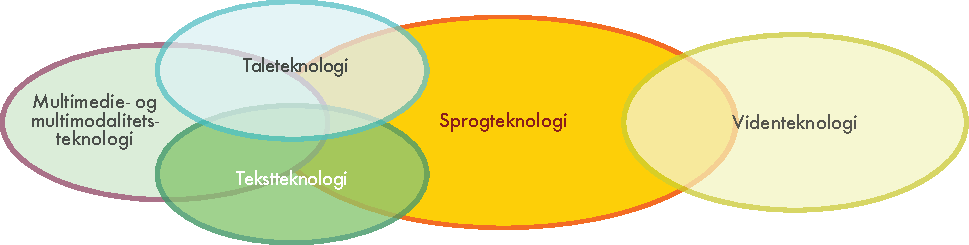
\includegraphics[width=\textwidth]{../_media/danish/language_technologies}
  \caption{Sprogteknologi i kontekst}
  \label{fig:ltincontext_de}
  \colorrule{grey3}{\textwidth}{1.5pt}
\end{figure*}

I vores kommunikation kombinerer vi sprog med andre former for kommunikation og andre informationskanaler. Fx kan tale inddrage gestik og ansigtsudtryk. Digitale tekster er forbundet med billeder og lyd. Film kan indeholde b\aa de skrevet og talt sprog. Tale- og tekstteknologi overlapper og interagerer \mbox{alts\aa} med megen anden teknologi som indg\aa r i behandlingen af multimodal kommunikation og multimediefiler.

I det f\o lgende vil vi diskutere sprogteknologiens vigtigste anvendelsesomr\aa der, dvs.\ sprogkontrol, informationss\o gning \mbox{p\aa} nettet, taleteknologi og maskinovers\ae ttelse. Dette inkluderer softwaresystemer og basisteknologier som 

\begin{itemize}
      \item stavekontrol
      \item forfatterst\o tte
      \item computerst\o ttet sprogindl\ae ring
      \item informationss\o gning
      \item videnuddragelse
      \item tekstresumering
      \item sp\o rgsm\aa l/svar
      \item talegenkendelse
      \item talesyntese
    \end{itemize}
    \sloppy
Sprogteknologi er et etableret forskningsomr\aa de med en omfattende m\ae ngde af introducerende litteratur. Den interesserende l\ae ser henvises til f\o lgende refe\-rencer:  \cite{Braasch, jurafsky-martin01, manning-schuetze1, lt-world1, lt-survey1}.   


 F\o r vi diskuterer disse anvendelses\-omr\aa der, vil vi kort beskrive arkitekturen i et typisk sprogteknologisk system.


\subsection{Systemarkitektur}

 Software til natursprogsbehandling best\aa r typisk af flere komponenter der afspejler forskellige aspekter af sproget.  Figur~\ref{fig:textprocessingarch_de} viser en meget forenklet arkitektur for et typisk system til behandling af tekst. De f\o rste tre mo\-duler besk\ae ftiger sig med tekstinputtets struktur og betydning:

\begin{figure*}[hb]
  \colorrule{grey3}{\textwidth}{1.5pt}
  \center
  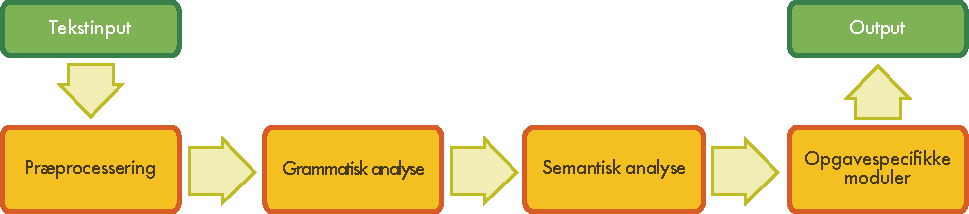
\includegraphics[width=\textwidth]{../_media/danish/text_processing_app_architecture}
  \caption{Arkitekturen for et typisk system til behandling af tekst}
  \label{fig:textprocessingarch_de}
  \colorrule{grey3}{\textwidth}{1.5pt}
\end{figure*}

\begin{enumerate}
  \item Pr\ae processering: rydder op i data, fjerner formate\-ring, genkender inputsproget osv.
      \item Grammatisk analyse: finder verbet og dets objekter, attributive led og andre ordklasser samt afd\ae kker s\ae tningsstrukturen.
      \item Semantisk analyse: entydigg\o r (beregner den korrekte betydning af et ord i en given kontekst); afg\o r hvad anaforer og refererende udtryk som {\it hun}, {\it bilen} osv.\ refererer til; og udtrykker s\ae tningens betydning i en maskinl\ae sbar form.
\end{enumerate}

N\aa r teksten er analyseret, kan opgavespecifikke mo\-duler udf\o re fx automatisk resumering og databaseopslag. Dette er en forsimplet beskrivelse af systemarkitekturen og kompleksiteten ved sprogteknologiske systemer.

Introduktionen til sprogteknologiens centrale anvendelsesomr\aa der efterf\o lges af et kort overblik over sprogteknologisk forskning og uddannelse i dag og afsluttes med en oversigt over tidligere og nuv\ae rende forskningsprogrammer. \mbox{Derp\aa} vil vi pr\ae sentere en ekspertbed\o mmelse af vigtige sprogteknologiske v\ae rkt\o jer og resurser m\aa lt \mbox{p\aa} flere dimensioner s\aa som tilg\ae ngelighed, modenhed og kvalitet. Den generelle situation for sprogteknologi for dansk bliver opsummeret i en tabel (figur~\ref{fig:lrlttable_de}) \mbox{p\aa} side~\pageref{fig:lrlttable_de}. V\ae rkt\o jer og resurser som er skrevet med fed i teksten, optr\ae der \mbox{ogs\aa} i figur~\ref{fig:lrlttable_de} i slutningen af dette kapitel. Her sammenlignes \mbox{ogs\aa} sprogteknologist\o tte til dansk med de \o vrige europ\ae iske sprog som beskrives i denne hvidbogsserie.


\subsection{Centrale udviklingsområder} 

I dette afsnit s\ae tter vi fokus \mbox{p\aa} de vigtigste sprogteknologiske v\ae rkt\o jer og resurser og giver en oversigt over sprogteknologiske aktiviteter i Danmark. 


\subsubsection{Sprogkontrol}

\begin{figure*}[htb]
  \colorrule{grey3}{\textwidth}{1.5pt}
  \center
  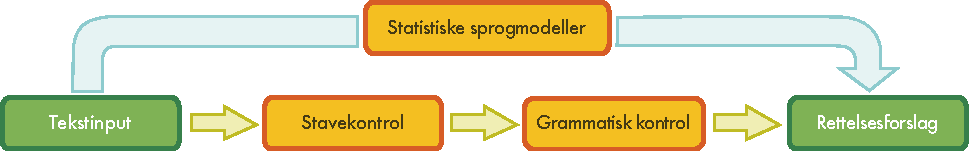
\includegraphics[width=\textwidth]{../_media/danish/language_checking}
  \caption{Sprogkontrol (statistisk; regelbaseret)}
  \label{fig:langcheckingaarch_de}
  \colorrule{grey3}{\textwidth}{1.5pt}
\end{figure*}

Alle der har anvendt et tekstbehandlingssystem som Microsoft Word, ved at det har en stavekontrol som mar\-kerer stavefejl og foresl\aa r rettelser. De f\o rste stavekontrolprogrammer sammenlignede dokumentets ord med en ordbogs korrekt stavede ord. I dag er disse programmer langt mere avancerede. Ved at anvende sprogafh\ae ngige algoritmer til {\bf grammatisk analyse} finder de b\aa de fejl der har relation til morfologi (fx flertalsdannelse) og til syntaks s\aa som et manglende verbum eller kongruensfejl mellem subjekt og verbal (fx {\it hun *skrive et brev}), men mange stavekontroller vil fx ikke finde fejl i f\o lgende engelske tekst \cite{zar1}:

\begin{quote}
 {\it  I have a spelling checker,\\
  It came with my PC.\\
  It plane lee marks four my revue\\
  Miss steaks aye can knot sea.}
\end{quote}

S\aa danne fejl kr\ae ver normalt en analyse af konteksten. Denne type analyse bygger enten \mbox{p\aa} sprogspecifikke {\bf grammatikker} som eksperter har kodet ind i softwaren, eller \mbox{p\aa} en statistisk sprogmodel. I sidstn\ae vnte model beregnes sandsynligheden for at et bestemt ord optr\ae der i en bestemt position. Fx er {\it stort hus}  en langt mere sandsynlig ordsekvens end {\it stor hus}. En statistisk sprogmodel kan laves automatisk ved at anvende en stor m\ae ngde (korrekte) sproglige data (et s\aa kaldt {\bf tekstkorpus}). Hovedparten af de systemer som anvender disse to fremgangsm\aa der, er blevet udviklet med engelske data. 

Ingen af de to modeller kan let overf\o res til det danske sprog med dets s\ae rlige karakteristika som kompositumdannelse og et rigere b\o jningssystem. Derfor var det en alvorlig fejl ved de f\o rste danske stavekontroller at de ukorrekt fejlmarkerede produktive komposita som fx {\it pasningsordning}. Hvis et s\aa dant kompositum ikke var leksikaliseret i en ordbog eller \mbox{p\aa} en ordliste (hvilket produktive komposita normalt ikke er), medf\o rte det en fejlmarkering. Disse fejlagtige markeringer skyldtes at der endnu ikke fandtes gode kompositum-opdelingsprogrammer som kunne tjekke hvert enkelt ord i kompositummet. Desv\ae rre har denne mangel i de tidlige stavekontroller f\o rt til en stigning i antallet af stavefejl; folk er under indflydelse dels af at sammensatte ord \mbox{p\aa} engelsk i reglen skrives i to ord, dels af det faktum at det ikke f\o rer til fejlmarkering med en dansk stavekontrol hvis et dansk sammensat ord skrives i to ord.  De seneste stavekontroller for dansk er blevet forbedret \mbox{p\aa} dette punkt.

Danske grammatiktjekkere er derimod stadig \mbox{p\aa} et temmelig tidligt stadie. De er generelt i stand til at finde simple grammatiske fejl s\aa som konkordansfejl inden for kort afstand som i {\it *den r\o de hus}, mens andre grammatiske fejl ikke identificeres, som fx {\it *jeg var kede af du ikke kom}.
%
OpenOffice er \mbox{ogs\aa} begyndt at levere v\ae rkt\o jer til sprogkontrol af dansk; Magenta  har integreret flere danske open-source leksikalske resurser i dokumentbehandlingsv\ae rkt\o jet, bl.a.\ synonymopslag.

Med s\ae rligt henblik \mbox{p\aa} undervisning er Mikro V\ae rkstedet en af hovedakt\o rerne \mbox{p\aa} markedet for digitale undervisningshj\ae lpemidler, heriblandt l\ae sev\ae rkt\o jer for ordblinde og skrivehj\ae lp. Desuden b\o r Ordbogen.com n\ae vnes fordi de giver adgang til mange forskellige online ordb\o ger. 

\boxtext{Sprogkontrol er ikke begr\ae nset til tekstbehandlingssystemer; det bruges \mbox{ogs\aa} i forfatterv\ae rkt\o jer.}

Brugen af sprogkontrol er ikke begr\ae nset til tekstbehandlingssystemer; det bruges \mbox{ogs\aa} i ``forfatterv\ae rkt\o jer'', som is\ae r anvendes til skrivning af manualer og anden dokumentation for avanceret it, sundhed, teknik og lignende som skrives efter s\ae rlige standarder. Kundeklager over forkert brug og erstatningskrav som et resultat af d\aa rligt forst\aa et instruktion har motiveret virksomhederne til at prioritere kvaliteten af den tekniske dokumentation samtidig med at de henvender sig til det internationale marked (via overs\ae ttelse eller lokalise\-ring). Fremskridtene inden for natursprogsbehandling \aa bner mulighed for udvikling af forfatterv\ae rkt\o jer som hj\ae lper forfattere af teknisk dokumentation med at bruge det ordforr\aa d og den s\ae tningsstruktur der er i overensstemmelse med branchens retningslinjer og (virksomhedens) terminologi.

Udover stavekontrol og forfatterhj\ae lp er sprogkontrol \mbox{ogs\aa} vigtig inden for computerst\o ttet sprogindl\ae ring. Og sprogkontrolprogrammer anvendes \mbox{ogs\aa} til automatisk korrektion af foresp\o rgsler i browsere, som man ser det i Googles {\it Did you mean~\dots}-forslag.

\subsubsection{Internets\o gning}

S\o gning \mbox{p\aa} internettet, \mbox{p\aa} intranet og i digitale bi\-blioteker udg\o r i dag sandsynligvis den hyppigste anvendelse af sprogteknologi, og dog er denne anvendelse i det store og hele underudviklet. Googles s\o gemaskine som blev lanceret i 1998, behandler nu 80\% af alle foresp\o rgsler \cite{spi1}.   Verbet {\it at google} har endda en indgang i Den Danske Ordbog. Google-s\o gegr\ae nsefladen og dens resultatsider er ikke blevet \ae ndret v\ae sentligt siden den f\o rste version. Men den nuv\ae rende version giver mulighed for korrektion af stavefejl og har inkorporeret grundl\ae ggende semantiske s\o gemuligheder som kan forbedre n\o jagtigheden af s\o gningen ved at analysere betydningen af termer i en s\o gekontekst \cite{pc1}.   Googles succeshistorie viser at en stor m\ae ngde tilg\ae ngelige data og effektive indekseringsteknikker kan give tilfredsstillende resultater ved at bruge en statistisk baseret fremgangsm\aa de.

\begin{figure*}[t]
  \colorrule{grey3}{\textwidth}{1.5pt}
  \center
  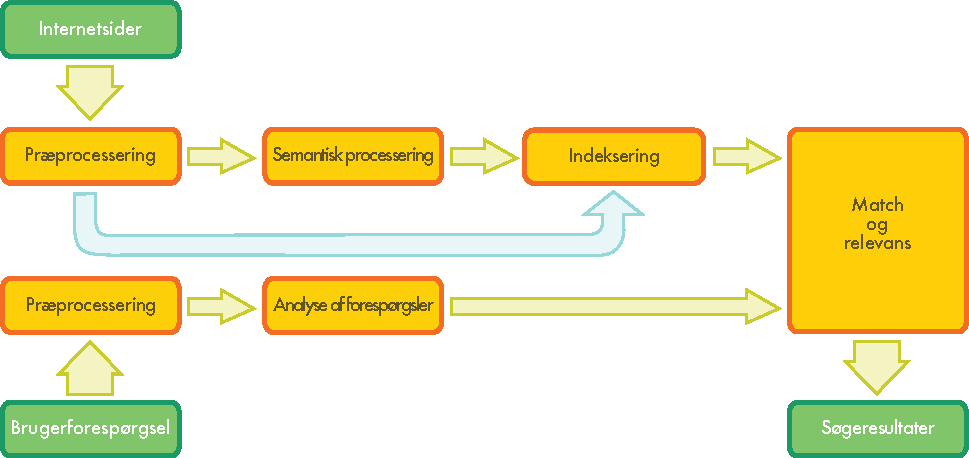
\includegraphics[width=\textwidth]{../_media/danish/web_search_architecture}
  \caption{Internetsøgning}
  \label{fig:websearcharch_de}
  \colorrule{grey3}{\textwidth}{1.5pt}
\end{figure*}

Avanceret informationss\o gning kr\ae ver at man inte\-grerer mere lingvistisk viden for at kunne udf\o re tekst\-forst\aa else. Fors\o g med systemer der anvender {\bf leksikalske resurser} som maskinl\ae sbare thesauri eller ontologiske sprogresurser (fx Princeton WordNet for engelsk eller det tilsvarende danske wordnet, DanNet), har forbedret deres s\o geresultater ved at bruge sy\-nonymer for de originale s\o getermer (fx {\it autoforsikring}, {\it bilforsikring} og {\it kaskoforsikring} eller endnu mere l\o st relaterede termer). 

\boxtext{Den n\ae ste generation af s\o gemaskiner skal indeholde meget mere avanceret sprogteknologi.}

Den n\ae ste generation af s\o gemaskiner skal indeholde meget mere avanceret sprogteknologi, is\ae r for at kunne h\aa ndtere s\o gninger formuleret som sp\o rgsm\aa l eller andre s\ae tningstyper i stedet for en liste af n\o gleord. S\o gningen {\it Giv mig en liste over alle virksomheder som er blevet overtaget af andre virksomheder inden for de seneste fem \aa r} kr\ae ver en syntaktisk og {\bf semantisk analyse}. Systemet skal \mbox{ogs\aa} levere et indeks for at kunne frems\o ge de relevante dokumenter i en fart. Et tilfredsstillende svar vil kr\ae ve syntaktisk parsing for at kunne analysere s\ae tningens grammatiske struktur og afg\o re at brugeren er interesseret i virksomheder der er blevet opk\o bt, ikke virksomheder der har opk\o bt andre virksomheder. Hvad ang\aa r udtrykket {\it de seneste fem \aa r} skal systemet afg\o re hvilke \aa r der er relevante. Og s\o gningen skal matches mod et v\ae ldigt stort antal ustruktu\-rerede data for at finde frem til den relevante information som brugeren er interesseret i. Dette kaldes informationss\o gning og involverer frems\o gning og priorite\-ring af relevante dokumenter. For at kunne generere en liste af virksomheder skal systemet desuden kunne identificere et virksomhedsnavn i et dokument, en proces der kaldes ``navnegenkendelse''.

En mere kr\ae vende udfordring er at matche en foresp\o rgsel i \'{e}t sprog med dokumenter i et andet. Tv\ae rsproglig informationss\o gning involverer automatisk overs\ae ttelse af foresp\o rgslen til alle mulige sprog og \mbox{derp\aa} overs\ae ttelse af resultaterne tilbage til det sprog brugeren anvender.

Nu da data i stadig h\o jere grad findes i ikke-tekstlige formater, er der behov for tjenester der kan h\aa ndtere multimedie-informationss\o gning i billeder, lydfiler og videodata. Lyd- og videofiler kr\ae ver et talegen\-kendelsesmodul for at omdanne tale til tekst (eller til en fonetisk repr\ae sentation), som \mbox{s\aa} kan matches med en brugerforesp\o rgsel. 

\mbox{Sm\aa} og mellemstore virksomheder (SMV'er) i Danmark som Ankiro, ScanJour, LAT Consulting, Findwise, RDFined og andre udvikler og anvender med succes s\o geteknologier der er skr\ae ddersyet til s\ae rlige virksomhedsbehov. Udviklingsarbejdet hos fx Ankiro har fokus \mbox{p\aa} avancerede s\o gemaskiner til emnespecifikke portaler ved at udnytte emnerelevant semantik. Pga.\ de store krav til computerkraft er disse s\o gemaskiner kun \o konomisk anvendelige \mbox{p\aa} relativt \mbox{sm\aa} korpusser. Processeringstiden kan let overstige den tid en almindelig statistisk s\o gemaskine, som fx Google, ville bruge. Disse s\o gemaskiner stiller \mbox{ogs\aa} h\o je krav til dom\ae nespecifik modellering hvilket g\o r det umuligt at anvende disse mekanismer \mbox{p\aa} hele internettet. Desuden er de teknologier der udvikles i disse sammenh\ae nge, generelt ikke offentligt tilg\ae ngelige for yderligere forskning og udvikling. Mange danske hjemmesider linker til en Google-s\o gemaskine som den eneste s\o gefacilitet pga.\ praktiske forhindringer af denne art.

Eksperimentelle, ontologibaserede s\o ge\-maskiner er blevet udviklet af flere danske universiteter, bl.a.\ Roskilde Universitet. OntoQuery og SIABO prototyperne er eksempler \mbox{p\aa} s\aa danne eksperimentelle s\o gemaskiner som arbejder \mbox{p\aa} mindre dom\ae ner med en rig ontologisk repr\ae sentation.   Men disse kan ikke umiddelbart skaleres op til st\o rre dom\ae ner.
  
\subsubsection{Taleteknologi}

\begin{figure*}[hb]
  \colorrule{grey3}{\textwidth}{1.5pt}
  \center 
  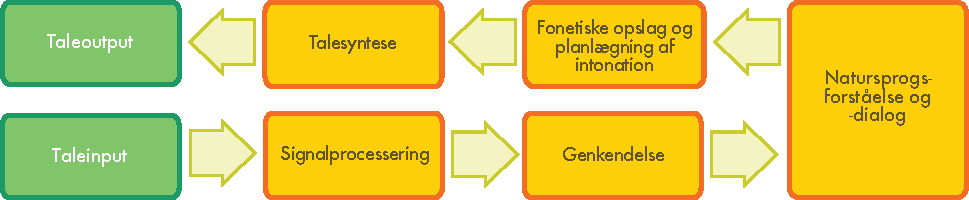
\includegraphics[width=\textwidth]{../_media/danish/simple_speech-based_dialogue_architecture}
  \caption{Talebaseret dialogarkitektur}
  \label{fig:dialoguearch_de}
  \colorrule{grey3}{\textwidth}{1.5pt}
\end{figure*}

 Taleteknologi handler om at skabe gr\ae nseflader som giver brugere mulighed for at arbejde interaktivt i talt sprog i stedet for at anvende grafisk display, tastatur og mus. I dag anvender virksomheder stemmestyrede gr\ae nseflader (VUI) som regel til halv- eller fuldautomatisk telefonservice for deres kunder, ansatte og partnere. Forretningsomr\aa der der er meget afh\ae ngige af VUI-systemer, indbefatter bankverdenen, leverand\o rk\ae der, offentlig transport og telekommunikation. Anden brug af taleteknologi omfatter gr\ae nseflader til bilnavigations\-systemer og brug af talt sprog som alternativ til grafiske gr\ae nseflader eller touch-screen-gr\ae nseflader i smart\-phones. 

Taleteknologi omfatter fire teknologier:

\begin{enumerate}
  \item Automatisk {\bf talegenkendelse} afg\o r hvilke ord der bliver sagt i en given sekvens af lyde udtalt af en bruger.
      \item Natursprogsforst\aa else analyserer den syntaktiske struktur i en brugerytring og fortolker den i henhold til det p\aa g\ae ldende system.
      \item  Dialogstyring afg\o r hvilken handling der skal udf\o res, afh\ae ngig af brugerinputtet og systemfunktionaliteten.
      \item {\bf Talesyntese} (tekst til tale eller TTS) omdanner sy\-stemets svar til lyde for brugeren.
\end{enumerate}

  En af de st\o rste udfordringer for automatiske talegen\-kendelsessystemer er pr\ae cis genkendelse af brugerens ord. Det betyder at man \mbox{m\aa} begr\ae nse omfanget af brugerens ytringer til en liste af n\o gleord eller manuelt udvikle sprogmodeller som d\ae kker et stort udvalg af natursprogsytringer. Ved at anvende maskinl\ae rings\-teknikker kan sprogmodeller \mbox{ogs\aa} genereres automatisk ud fra {\bf talesprogskorpusser}, dvs.\ store samlinger af tale-lydfiler og teksttranskriptioner. Begr\ae nsning af mulige ytringer vil normalt betyde en ufleksibel anvendelse af gr\ae nsefladen og kan \mbox{g\aa} ud over brugernes accept; men at skabe, tune og vedligeholde detaljerede sprogmodeller vil \o ge omkostningerne betydeligt. VUI'er som anvender sprogmodeller, og som tillader brugeren at udtrykke sit \o nske \mbox{p\aa} noget der minder om natursprog --~tilskyndet af en {\it Hvordan kan jeg hj\ae lpe dig?}-hilsen~-- bliver ofte bedre accepteret af brugeren.

\boxtext{Taleteknologi udg\o r grundlaget for gr\ae nseflader som giver brugere mulighed for at arbejde interaktivt i talt sprog.}

Virksomheder anvender ofte svar som er indtalt af professionelle talere, til at generere output til den stemmestyrede gr\ae nseflade. Ved faste ytringer hvor ordvalget ikke afh\ae nger af en s\ae rlig brugskontekst eller af personlige brugerdata, kan dette give en rigtig god brugeroplevelse. Men et mere dynamisk indhold i en ytring vil lide under den unaturlige intonation fordi stumper af lydfiler simpelthen er blevet klippet sammen. Talesyntesesystemer i dag bliver bedre og bedre (sk\o nt de kan blive endnu bedre) til at producere naturligt lydende dynamiske ytringer.

\mbox{P\aa} markedet for taleinteraktionsteknologi er gr\ae nsefladerne i l\o bet af de seneste ti \aa r blevet st\ae rkt standardiserede hvad ang\aa r de forskellige teknologiske komponenter. Der er \mbox{ogs\aa} sket en kraftig markedskonsoli\-dering inden for talegenkendelse og talesyntese. De nationale markeder i G20-landene  (\o konomisk robuste lande med store befolkninger) er blevet domineret af bare fem globale akt\o rer med Nuance (USA) og Loquendo (Italien) som de st\o rste akt\o rer i Europa. I 2011 annoncerede Nuance overtagelsen af Loquendo hvilket udg\o r endnu et skridt i markedskonsolideringen. 

\mbox{P\aa} det danske marked for taleteknologiske l\o sninger er der
et antal nationale firmaer (Mikro V\ae rkstedet, Prolog Development
Center, Max Manus samt IBM og Siemens Danmark) der har specialiseret
sig i udvikling af l\o sninger baseret \mbox{p\aa} taleteknologier fra
de internationale teknologileverand\o rer. Nuance er den
altdominerende internationale taleteknologileverand\o r med
dansksproget taleteknologi. \mbox{S\aa} godt som samtlige
taleteknologier der kan genkende og udtale dansk, er opk\o bt af
Nuance over de sidste 5-6 \aa r, fx Philips SpeechMagic, Loquendo og
SVOX.

Af basisteknologier der kan genkende dansk sprog, findes pt.\ Nuance
SpeechMagic og Nuance Dragon Development Platform (cloud
baseret). \mbox{P\aa} disse teknologier har Max Manus udviklet en l\o
sning prim\ae rt til sygehussektoren, IBM en l\o sning til den
kommunale sektor og Prolog Development Center standardsystemet Dictus
samt skr\ae ddersyede l\o sninger til Folketingstidende og de to
nationale TV-stationer. Nuance selv leverer gratis App's Dragon
Dictation og Dragon Search til iPhone/iPad mens Prolog Development
Center leverer Dictus til Android. Talegenkendere til telefoni er
reduceret til \'{e}n basisleverand\o r, Nuance. Siemens Danmark og
Prolog Development Center er de danske firmaer der har leveret
talestyret telefontjeneste \mbox{p\aa} Nuance Recognizer v9. Der udbydes over 10 forskellige danske stemmer til talesyntese fra
firmaerne Nuance (inkl.\ Loquendo og SVOX), Acapela og det danske firma
Mikro V\ae rkstedet. Desuden planl\ae gger det succesfulde polske
firma IVONA at lancere et antal danske stemmer i starten af 2012.

Et stigende antal af de store internationale leverand\o rer af
forbrugerelektronik (Garmin, Navigon, Samsung) tilbyder produkter hvor
der er indbygget dansk talegenkendelse \mbox{s\aa} produkterne kan
styres med stemmen. Et endnu st\o rre antal produkter, fx iRobot, har
\mbox{ogs\aa} indbygget dansk talesyntese. Et lille men stigende antal
danske producenter af forbrugerprodukter har indbygget dansk
taleteknologi, fx 6th Sense Solution til opl\ae sning af
busstoppesteder og CIM Interconn til opl\ae sning af sk\ae
rminformation \mbox{p\aa} plejecentre.

Hvad ang\aa r anvendelsen af stemmestyrede gr\ae nseflader, er eftersp\o rgslen steget voldsomt de seneste fem \aa r. Denne tendens er drevet af kundernes stigende eftersp\o rgsel \mbox{p\aa} selvbetjening og den betydelige udgiftsoptimering som automatisk telefonservice giver, sammen med en v\ae sentligt \o get accept af talt sprog som en mulighed for menneske-maskine-interaktion.

I fremtiden vil der komme store forandringer med smartphones som en ny platform til adminstration af kunderelationer foruden fastnettelefoner, internettet og e-mail. Det vil \mbox{ogs\aa} p\aa virke brugen af taleinteraktionsteknologien. \mbox{P\aa} langt sigt vil der blive f\ae rre telefonbaserede stemmestyrede brugergr\ae nseflader, og talt sprog vil spille en langt mere central rolle som et brugervenligt input til smartphones. Det vil i det store og hele dreje sig om trin for trin-forbedringer af n\o jagtigheden i den taleruafh\ae ngige talegenkendelse via dikteringssy\-stemer som allerede nu tilbydes som centrale tjenester for smartphonebrugere.

\subsubsection{Maskinovers\ae ttelse}

Ideen med at anvende digitale computere til overs\ae ttelse af natursprog g\aa r tilbage til 1946 og blev fulgt op af betydelige forskningsbevillinger i 1950'erne og igen i 1980'erne. {\bf Maskinovers\ae ttelse} (MT) kan dog stadig ikke leve op til det indledende l\o fte om fuldst\ae ndig automatiseret overs\ae ttelse.

\boxtext{Den mest basale frem\-gangs\-m\aa de til\\ maskin\-over\-s\ae ttelse er at erstatte ordene i en\\[.3mm] tekst \mbox{p\aa} \'{e}t  sprog med ord fra et andet sprog.}

Den mest basale fremgangsm\aa de til maskinovers\ae ttelse er at erstatte ordene i en tekst \mbox{p\aa} \'{e}t  sprog med ord fra et andet sprog. Denne fremgangsm\aa de kan stadig anvendes inden for emneomr\aa der som har et meget begr\ae nset, formelagtigt sprog, som fx vejrudsigter. En god overs\ae ttelse af tekster som er knap \mbox{s\aa} standardiserede, kr\ae ver at st\o rre tekstenheder (fraser, s\ae tninger og endda hele afsnit) matches med deres n\ae rmeste \ae kvivalenter \mbox{p\aa} m\aa lsproget. Den st\o rste vanskelighed ligger i at menneskesprog er flertydigt. Flertydighed skaber udfordringer \mbox{p\aa} flere niveauer, som entydigg\o relse af ord \mbox{p\aa} det leksikalske plan (en {\it jaguar} er et bilm\ae rke eller et dyr) eller afg\o relse af hvortil et led h\o rer, som i eksemplet nedenfor hvor {\it med en kikkert} kan referere til enten {\it jeg} eller {\it mand}:

\begin{itemize}
\item {\it Jeg \mbox{s\aa} en mand med en kikkert.}
\end{itemize}

En m\aa de at bygge MT-systemer \mbox{p\aa} er at anvende lingvi\-stiske regler. N\aa r man overs\ae tter mellem t\ae t besl\ae g\-tede sprog, kan direkte udskiftning af ordene v\ae re en fornuftig metode. Men regelbaserede maskinovers\ae ttelsessystemer analyserer som oftest inputteksten og danner en midlertidig symbolsk repr\ae sentation, hvorfra teksten kan genereres \mbox{p\aa} m\aa lsproget. Om denne metode giver succes, afh\ae nger helt af om der er store ordb\o ger med morfologisk, syntaktisk og semantisk information til disposition samt store m\ae ngder af omhyggeligt opbyggede grammatiske regler udarbejdet af dygtige lingvister. Det er en meget lang og derfor meget kostbar proces.

\begin{figure*}[htb]
  \colorrule{grey3}{\textwidth}{1.5pt}
  \center
  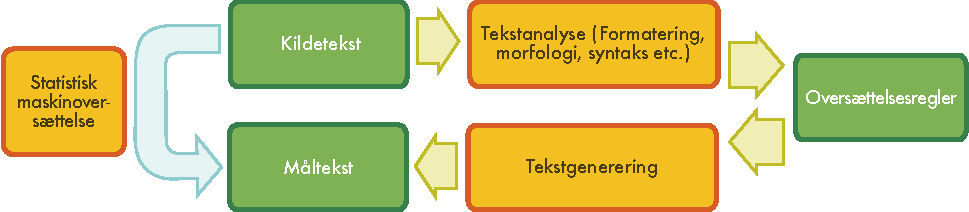
\includegraphics[width=\textwidth]{../_media/danish/machine_translation}
  \caption{Maskinovers\ae ttelse (statistisk; regelbaseret)}
  \label{fig:mtarch_de}
  \colorrule{grey3}{\textwidth}{1.5pt}
\end{figure*}

I slutningen af 1980'erne da computerkraften \o gedes og blev billigere, var der stigende interesse for stati\-stiske modeller til maskinovers\ae ttelse. Statistiske mo\-deller stammer fra analyser af {\bf parallelle korpusser} som fx det parallelle korpus Europarl som indeholder udskrifter fra Europaparlamentets m\o der \mbox{p\aa} 21 EU-sprog. Hvis der er data nok, er statistisk MT godt nok til at udlede en omtrentlig betydning af en tekst \mbox{p\aa} et fremmedsprog ved at behandle parallelle versioner og finde sandsynlige m\o nstre af ord. Men i mods\ae tning til regelbaserede sy\-stemer genererer statistisk MT ofte et ugrammatisk output. Statistisk MT har den fordel at det kr\ae ver f\ae rre menneskelige resurser, og det kan \mbox{ogs\aa} tage h\o jde for s\ae rlige karakteristika i et sprog (fx idiomatiske udtryk) som ofte bliver overset i regelbaserede systemer. 

Styrkerne og svaghederne ved regelbaseret og statistisk maskinovers\ae ttelse har en tilb\o jelighed til at v\ae re komplement\ae re, \mbox{s\aa} forskere nu til dags fokuserer \mbox{p\aa} hybride fremgangsm\aa der der kombinerer de to metoder. \'{E}n metode anvender b\aa de regelbaserede og statistiske systemer sammen med et udv\ae lgelsesmodul som afg\o r hvad der er det bedste output for hver s\ae tning. Men resultaterne for s\ae tninger som er l\ae ngere end fx 12 ord, er som regel ikke s\ae rligt gode. Det er en bedre l\o sning at kombinere de bedste dele af hver s\ae tning fra mange forskellige output; dette er en ret kompliceret proces da det ikke altid er indlysende hvilke dele der passer sammen i de forskellige alternative s\ae tninger. De skal f\o rst aligneres.

Maskinovers\ae ttelse er en s\ae rlig udfordring for dansk. Muligheden for at danne nye komposita g\o r ordbogsanalyse og -d\ae kning vanskelig; de mange partikelverber udg\o r et problem for analysen, og udbredt leksikalsk flertydighed vanskeligg\o r  entydigg\o relsen af ord. 

Bortset fra PaTrans (et engelsk-dansk patentovers\ae ttelsessystem) blev de tidlige MT-systemer for dansk, som SYSTRAN-prototypen, prim\ae rt udviklet af udenlandske virksomheder. Alle disse systemer var regelbaserede. Der foreg\aa r en ganske betydelig forsk\-ning i MT-teknologi i b\aa de nationale og internationale sammenh\ae nge, og der findes nogle nye danske virksomheder (som fx Grammar Soft  og Languagelens) der leverer regelbaserede og statistiske maskinovers\ae ttelsessystemer for dansk. St\o rstedelen af de lettilg\ae ngelige systemer for dansk, som fx Google Translate og ESTeam Translator, bliver dog stadig udviklet i udlandet.

\boxtext{Maskinovers\ae ttelse er en\\[.3mm] s\ae rlig udfordring for dansk.} 

Der er stadig et k\ae mpestort potentiale i at forbedre MT-systemernes kvalitet. Udfordringerne indeb\ae rer at man tilpasser de sproglige resurser til det aktuelle emne- eller brugeromr\aa de og integrerer teknologien i arbejdsgange der allerede omfatter termbaser og overs\ae ttelseshukommelser. Et andet problem er at de fleste nuv\ae rende sy\-stemer er centreret om engelsk og kun st\o tter nogle \mbox{f\aa} sprog fra og til dansk. Det skaber hindringer for overs\ae ttelsesprocessen og tvinger brugerne af MT til at l\ae re forskellige leksikalske kodningsv\ae rkt\o jer for de forskellige systemer. 

Evalueringskampagner hj\ae lper med at sammenligne kvaliteten af MT-systemerne, de forskellige fremgangsm\aa der og systemernes status for forskellige sprogpar. Tabel~\ref{fig:euromatrix_de} som blev lavet i EC Euromatrix+-projektet, viser resultaterne for 22 af de 23 officielle EU-sprog parvis. (Irsk blev ikke sammenlignet.) Resultaterne er ordnet efter BLEU-pointtal \cite{bleu1} som giver h\o jere tal for bedre overs\ae ttelser.   (En menneskelig overs\ae tter ville score omkring 80 point.)

De bedste resultater (med gr\o nt og bl\aa t) blev opn\aa et af sprog som nyder godt af en stor forskningsindsats i koordinerede forskningsprogrammer, og af at der findes mange parallelle korpusser for disse sprog (fx engelsk, fransk, hollandsk, spansk og tysk). Sprog med d\aa rligere resultater er vist med r\o dt. Disse sprog mangler enten forsknings- og udviklingsindsatser af denne art, eller \mbox{ogs\aa} er de strukturelt set meget anderledes end andre sprog (fx ungarsk, maltesisk og finsk).


\begin{figure*}[htbp]
  \centering
  \setlength{\tabcolsep}{0.17em}
  \small
  \begin{tabular}{>{\columncolor{corange1}}cccccccccccccccccccccccc}
    & \multicolumn{22}{>{\columncolor{corange1}}c}{M\aa lsprog -- \textcolor{grey1}{Target language}}\\\addlinespace[{-.009cm}]
    \rowcolor{corange1}  & EN & BG & DE & CS & DA & EL & ES & ET & FI & FR & HU & IT & LT & LV & MT & NL & PL & PT & RO & SK & SL & SV\\
    EN & -- & \textcolor{blue}{40.5} & \textcolor{blue}{46.8} & \textcolor{green2}{52.6} & \textcolor{green2}{50.0} & \textcolor{blue}{41.0} & \textcolor{green2}{55.2} & \textcolor{purple}{34.8} & \textcolor{purple}{38.6} & \textcolor{green2}{50.1} & \textcolor{purple}{37.2} & \textcolor{green2}{50.4} & \textcolor{purple}{39.6} & \textcolor{blue}{43.4} & \textcolor{purple}{39.8} & \textcolor{green2}{52.3} & \textcolor{blue}{49.2} & \textcolor{green2}{55.0} & \textcolor{blue}{49.0} & \textcolor{blue}{44.7} & \textcolor{green2}{50.7} & \textcolor{green2}{52.0}\\
    BG & \textcolor{green}{61.3} & -- & \textcolor{purple}{38.7} & \textcolor{purple}{39.4} & \textcolor{purple}{39.6} & \textcolor{purple}{34.5} & \textcolor{blue}{46.9} & \textcolor{red3}{25.5} & \textcolor{red3}{26.7} & \textcolor{blue}{42.4} & \textcolor{red3}{22.0} & \textcolor{blue}{43.5} & \textcolor{red3}{29.3} & \textcolor{red3}{29.1} & \textcolor{red3}{25.9} & \textcolor{blue}{44.9} & \textcolor{purple}{35.1} & \textcolor{blue}{45.9} & \textcolor{purple}{36.8} & \textcolor{purple}{34.1} & \textcolor{purple}{34.1} & \textcolor{purple}{39.9}\\
    DE & \textcolor{green2}{53.6} & \textcolor{red3}{26.3} & -- & \textcolor{purple}{35.4} & \textcolor{blue}{43.1} & \textcolor{purple}{32.8} & \textcolor{blue}{47.1} & \textcolor{red3}{26.7} & \textcolor{red3}{29.5} & \textcolor{purple}{39.4} & \textcolor{red3}{27.6} & \textcolor{blue}{42.7} & \textcolor{red3}{27.6} & \textcolor{purple}{30.3} & \textcolor{red2}{19.8} & \textcolor{green2}{50.2} & \textcolor{purple}{30.2} & \textcolor{blue}{44.1} & \textcolor{purple}{30.7} & \textcolor{red3}{29.4} & \textcolor{purple}{31.4} & \textcolor{blue}{41.2}\\
    CS & \textcolor{green2}{58.4} & \textcolor{purple}{32.0} & \textcolor{blue}{42.6} & -- & \textcolor{blue}{43.6} & \textcolor{purple}{34.6} & \textcolor{blue}{48.9} & \textcolor{purple}{30.7} & \textcolor{purple}{30.5} & \textcolor{blue}{41.6} & \textcolor{red3}{27.4} & \textcolor{blue}{44.3} & \textcolor{purple}{34.5} & \textcolor{purple}{35.8} & \textcolor{red3}{26.3} & \textcolor{blue}{46.5} & \textcolor{purple}{39.2} & \textcolor{blue}{45.7} & \textcolor{purple}{36.5} & \textcolor{blue}{43.6} & \textcolor{blue}{41.3} & \textcolor{blue}{42.9}\\
    DA & \textcolor{green2}{57.6} & \textcolor{red3}{28.7} & \textcolor{blue}{44.1} & \textcolor{purple}{35.7} & -- & \textcolor{purple}{34.3} & \textcolor{blue}{47.5} & \textcolor{red3}{27.8} & \textcolor{purple}{31.6} & \textcolor{blue}{41.3} & \textcolor{red3}{24.2} & \textcolor{blue}{43.8} & \textcolor{red3}{29.7} & \textcolor{purple}{32.9} & \textcolor{red3}{21.1} & \textcolor{blue}{48.5} & \textcolor{purple}{34.3} & \textcolor{blue}{45.4} & \textcolor{purple}{33.9} & \textcolor{purple}{33.0} & \textcolor{purple}{36.2} & \textcolor{blue}{47.2}\\
    EL & \textcolor{green2}{59.5} & \textcolor{purple}{32.4} & \textcolor{blue}{43.1} & \textcolor{purple}{37.7} & \textcolor{blue}{44.5} & -- & \textcolor{green2}{54.0} & \textcolor{red3}{26.5} & \textcolor{red3}{29.0} & \textcolor{blue}{48.3} & \textcolor{red3}{23.7} & \textcolor{blue}{49.6} & \textcolor{red3}{29.0} & \textcolor{purple}{32.6} & \textcolor{red3}{23.8} & \textcolor{blue}{48.9} & \textcolor{purple}{34.2} & \textcolor{green2}{52.5} & \textcolor{purple}{37.2} & \textcolor{purple}{33.1} & \textcolor{purple}{36.3} & \textcolor{blue}{43.3}\\
    ES & \textcolor{green}{60.0} & \textcolor{purple}{31.1} & \textcolor{blue}{42.7} & \textcolor{purple}{37.5} & \textcolor{blue}{44.4} & \textcolor{purple}{39.4} & -- & \textcolor{red3}{25.4} & \textcolor{red3}{28.5} & \textcolor{green2}{51.3} & \textcolor{red3}{24.0} & \textcolor{green2}{51.7} & \textcolor{red3}{26.8} & \textcolor{purple}{30.5} & \textcolor{red3}{24.6} & \textcolor{blue}{48.8} & \textcolor{purple}{33.9} & \textcolor{green2}{57.3} & \textcolor{purple}{38.1} & \textcolor{purple}{31.7} & \textcolor{purple}{33.9} & \textcolor{blue}{43.7}\\
    ET & \textcolor{green2}{52.0} & \textcolor{red3}{24.6} & \textcolor{purple}{37.3} & \textcolor{purple}{35.2} & \textcolor{purple}{37.8} & \textcolor{red3}{28.2} & \textcolor{blue}{40.4} & -- & \textcolor{purple}{37.7} & \textcolor{purple}{33.4} & \textcolor{purple}{30.9} & \textcolor{purple}{37.0} & \textcolor{purple}{35.0} & \textcolor{purple}{36.9} & \textcolor{red3}{20.5} & \textcolor{blue}{41.3} & \textcolor{purple}{32.0} & \textcolor{purple}{37.8} & \textcolor{red3}{28.0} & \textcolor{purple}{30.6} & \textcolor{purple}{32.9} & \textcolor{purple}{37.3}\\
    FI & \textcolor{blue}{49.3} & \textcolor{red3}{23.2} & \textcolor{purple}{36.0} & \textcolor{purple}{32.0} & \textcolor{purple}{37.9} & \textcolor{red3}{27.2} & \textcolor{purple}{39.7} & \textcolor{purple}{34.9} & -- & \textcolor{red3}{29.5} & \textcolor{red3}{27.2} & \textcolor{purple}{36.6} & \textcolor{purple}{30.5} & \textcolor{purple}{32.5} & \textcolor{red2}{19.4} & \textcolor{blue}{40.6} & \textcolor{red3}{28.8} & \textcolor{purple}{37.5} & \textcolor{red3}{26.5} & \textcolor{red3}{27.3} & \textcolor{red3}{28.2} & \textcolor{purple}{37.6}\\
    FR & \textcolor{green}{64.0} & \textcolor{purple}{34.5} & \textcolor{blue}{45.1} & \textcolor{purple}{39.5} & \textcolor{blue}{47.4} & \textcolor{blue}{42.8} & \textcolor{green}{60.9} & \textcolor{red3}{26.7} & \textcolor{purple}{30.0} & -- & \textcolor{red3}{25.5} & \textcolor{green2}{56.1} & \textcolor{red3}{28.3} & \textcolor{purple}{31.9} & \textcolor{red3}{25.3} & \textcolor{green2}{51.6} & \textcolor{purple}{35.7} & \textcolor{green}{61.0} & \textcolor{blue}{43.8} & \textcolor{purple}{33.1} & \textcolor{purple}{35.6} & \textcolor{blue}{45.8}\\
    HU & \textcolor{blue}{48.0} & \textcolor{red3}{24.7} & \textcolor{purple}{34.3} & \textcolor{purple}{30.0} & \textcolor{purple}{33.0} & \textcolor{red3}{25.5} & \textcolor{purple}{34.1} & \textcolor{red3}{29.6} & \textcolor{red3}{29.4} & \textcolor{purple}{30.7} & -- & \textcolor{purple}{33.5} & \textcolor{red3}{29.6} & \textcolor{purple}{31.9} & \textcolor{red2}{18.1} & \textcolor{purple}{36.1} & \textcolor{red3}{29.8} & \textcolor{purple}{34.2} & \textcolor{red3}{25.7} & \textcolor{red3}{25.6} & \textcolor{red3}{28.2} & \textcolor{purple}{30.5}\\
    IT & \textcolor{green}{61.0} & \textcolor{purple}{32.1} & \textcolor{blue}{44.3} & \textcolor{purple}{38.9} & \textcolor{blue}{45.8} & \textcolor{blue}{40.6} & \textcolor{red3}{26.9} & \textcolor{red3}{25.0} & \textcolor{red3}{29.7} & \textcolor{green2}{52.7} & \textcolor{red3}{24.2} & -- & \textcolor{red3}{29.4} & \textcolor{purple}{32.6} & \textcolor{red3}{24.6} & \textcolor{green2}{50.5} & \textcolor{purple}{35.2} & \textcolor{green2}{56.5} & \textcolor{purple}{39.3} & \textcolor{purple}{32.5} & \textcolor{purple}{34.7} & \textcolor{blue}{44.3}\\
    LT & \textcolor{green2}{51.8} & \textcolor{red3}{27.6} & \textcolor{purple}{33.9} & \textcolor{purple}{37.0} & \textcolor{purple}{36.8} & \textcolor{red3}{26.5} & \textcolor{red3}{21.1} & \textcolor{purple}{34.2} & \textcolor{purple}{32.0} & \textcolor{purple}{34.4} & \textcolor{red3}{28.5} & \textcolor{purple}{36.8} & -- & \textcolor{blue}{40.1} & \textcolor{red3}{22.2} & \textcolor{purple}{38.1} & \textcolor{purple}{31.6} & \textcolor{purple}{31.6} & \textcolor{red3}{29.3} & \textcolor{purple}{31.8} & \textcolor{purple}{35.3} & \textcolor{purple}{35.3}\\
    LV & \textcolor{green2}{54.0} & \textcolor{red3}{29.1} & \textcolor{purple}{35.0} & \textcolor{purple}{37.8} & \textcolor{purple}{38.5} & \textcolor{red3}{29.7} & \textcolor{red2}{8.0} & \textcolor{purple}{34.2} & \textcolor{purple}{32.4} & \textcolor{purple}{35.6} & \textcolor{red3}{29.3} & \textcolor{purple}{38.9} & \textcolor{purple}{38.4} & -- & \textcolor{red3}{23.3} & \textcolor{blue}{41.5} & \textcolor{purple}{34.4} & \textcolor{purple}{39.6} & \textcolor{purple}{31.0} & \textcolor{purple}{33.3} & \textcolor{purple}{37.1} & \textcolor{purple}{38.0}\\
    MT & \textcolor{green}{72.1} & \textcolor{purple}{32.2} & \textcolor{purple}{37.2} & \textcolor{purple}{37.9} & \textcolor{purple}{38.9} & \textcolor{purple}{33.7} & \textcolor{blue}{48.7} & \textcolor{red3}{26.9} & \textcolor{red3}{25.8} & \textcolor{blue}{42.4} & \textcolor{red3}{22.4} & \textcolor{blue}{43.7} & \textcolor{purple}{30.2} & \textcolor{purple}{33.2} & -- & \textcolor{blue}{44.0} & \textcolor{purple}{37.1} & \textcolor{blue}{45.9} & \textcolor{purple}{38.9} & \textcolor{purple}{35.8} & \textcolor{blue}{40.0} & \textcolor{blue}{41.6}\\
    NL & \textcolor{green2}{56.9} & \textcolor{red3}{29.3} & \textcolor{blue}{46.9} & \textcolor{purple}{37.0} & \textcolor{blue}{45.4} & \textcolor{purple}{35.3} & \textcolor{blue}{49.7} & \textcolor{red3}{27.5} & \textcolor{red3}{29.8} & \textcolor{blue}{43.4} & \textcolor{red3}{25.3} & \textcolor{blue}{44.5} & \textcolor{red3}{28.6} & \textcolor{purple}{31.7} & \textcolor{red3}{22.0} & -- & \textcolor{purple}{32.0} & \textcolor{blue}{47.7} & \textcolor{purple}{33.0} & \textcolor{purple}{30.1} & \textcolor{purple}{34.6} & \textcolor{blue}{43.6}\\
    PL & \textcolor{green}{60.8} & \textcolor{purple}{31.5} & \textcolor{blue}{40.2} & \textcolor{blue}{44.2} & \textcolor{blue}{42.1} & \textcolor{purple}{34.2} & \textcolor{blue}{46.2} & \textcolor{red3}{29.2} & \textcolor{red3}{29.0} & \textcolor{blue}{40.0} & \textcolor{red3}{24.5} & \textcolor{blue}{43.2} & \textcolor{purple}{33.2} & \textcolor{purple}{35.6} & \textcolor{red3}{27.9} & \textcolor{blue}{44.8} & -- & \textcolor{blue}{44.1} & \textcolor{purple}{38.2} & \textcolor{purple}{38.2} & \textcolor{purple}{39.8} & \textcolor{blue}{42.1}\\
    PT & \textcolor{green}{60.7} & \textcolor{purple}{31.4} & \textcolor{blue}{42.9} & \textcolor{purple}{38.4} & \textcolor{blue}{42.8} & \textcolor{blue}{40.2} & \textcolor{green}{60.7} & \textcolor{red3}{26.4} & \textcolor{red3}{29.2} & \textcolor{green2}{53.2} & \textcolor{red3}{23.8} & \textcolor{green2}{52.8} & \textcolor{red3}{28.0} & \textcolor{purple}{31.5} & \textcolor{red3}{24.8} & \textcolor{blue}{49.3} & \textcolor{purple}{34.5} & -- & \textcolor{purple}{39.4} & \textcolor{purple}{32.1} & \textcolor{purple}{34.4} & \textcolor{blue}{43.9}\\
    RO & \textcolor{green}{60.8} & \textcolor{purple}{33.1} & \textcolor{purple}{38.5} & \textcolor{purple}{37.8} & \textcolor{blue}{40.3} & \textcolor{purple}{35.6} & \textcolor{green2}{50.4} & \textcolor{red3}{24.6} & \textcolor{red3}{26.2} & \textcolor{blue}{46.5} & \textcolor{red3}{25.0} & \textcolor{blue}{44.8} & \textcolor{red3}{28.4} & \textcolor{red3}{29.9} & \textcolor{red3}{28.7} & \textcolor{blue}{43.0} & \textcolor{purple}{35.8} & \textcolor{blue}{48.5} & -- & \textcolor{purple}{31.5} & \textcolor{purple}{35.1} & \textcolor{purple}{39.4}\\
    SK & \textcolor{green}{60.8} & \textcolor{purple}{32.6} & \textcolor{purple}{39.4} & \textcolor{blue}{48.1} & \textcolor{blue}{41.0} & \textcolor{purple}{33.3} & \textcolor{blue}{46.2} & \textcolor{red3}{29.8} & \textcolor{red3}{28.4} & \textcolor{purple}{39.4} & \textcolor{red3}{27.4} & \textcolor{blue}{41.8} & \textcolor{purple}{33.8} & \textcolor{purple}{36.7} & \textcolor{red3}{28.5} & \textcolor{blue}{44.4} & \textcolor{purple}{39.0} & \textcolor{blue}{43.3} & \textcolor{purple}{35.3} & -- & \textcolor{blue}{42.6} & \textcolor{blue}{41.8}\\
    SL & \textcolor{green}{61.0} & \textcolor{purple}{33.1} & \textcolor{purple}{37.9} & \textcolor{blue}{43.5} & \textcolor{blue}{42.6} & \textcolor{purple}{34.0} & \textcolor{blue}{47.0} & \textcolor{purple}{31.1} & \textcolor{red3}{28.8} & \textcolor{purple}{38.2} & \textcolor{red3}{25.7} & \textcolor{blue}{42.3} & \textcolor{purple}{34.6} & \textcolor{purple}{37.3} & \textcolor{purple}{30.0} & \textcolor{blue}{45.9} & \textcolor{purple}{38.2} & \textcolor{blue}{44.1} & \textcolor{purple}{35.8} & \textcolor{purple}{38.9} & -- & \textcolor{blue}{42.7}\\
    SV & \textcolor{green2}{58.5} & \textcolor{red3}{26.9} & \textcolor{blue}{41.0} & \textcolor{purple}{35.6} & \textcolor{blue}{46.6} & \textcolor{purple}{33.3} & \textcolor{blue}{46.6} & \textcolor{red3}{27.4} & \textcolor{purple}{30.9} & \textcolor{purple}{38.9} & \textcolor{red3}{22.7} & \textcolor{blue}{42.0} & \textcolor{red3}{28.2} & \textcolor{purple}{31.0} & \textcolor{red3}{23.7} & \textcolor{blue}{45.6} & \textcolor{purple}{32.2} & \textcolor{blue}{44.2} & \textcolor{purple}{32.7} & \textcolor{purple}{31.3} & \textcolor{purple}{33.5} & --\\
    \end{tabular}
  \caption{Maskinovers\ae ttelse mellem 22 EU-sprog --
    \textcolor{grey1}{Machine translation between 22 EU-languages \cite{euro1}}}
  \label{fig:euromatrix_de}
\end{figure*}

\subsection{Andre anvendelsesområder}

 Opbygningen af sprogteknologiske systemer indeb\ae rer en m\ae ngde mindre opgaver som ikke altid kan ses \mbox{p\aa} sy\-stemets overflade, men som leverer vigtige servicefunktionaliteter ``under k\o lerhjelmen'' til det p\aa g\ae ldende system. De udg\o r alle vigtige forskningsemner og har nu udviklet sig til individuelle subdiscipliner inden for datalingvistik.

%\boxtext{Sprachtechnologieanwendungen bieten häufig wichtige Servicefunktionen hinter den Kulissen %größerer Softwaresysteme.}

Sp\o rgsm\aa l/svar-systemer er fx et aktivt forskningsomr\aa de hvor der er blevet opbygget opm\ae rkede korpusser og igangsat videnskabelige konkurrencer. Begrebet sp\o rgsm\aa l/svar-systemer g\aa r ud over n\o gleordsbaserede s\o gninger (hvor s\o gemaskinen svarer ved at levere en samling potentielt relevante dokumenter) og s\ae tter brugeren i stand til at stille et konkret sp\o rgsm\aa l som systemet kan give et enkelt svar \mbox{p\aa}. Fx

\begin{itemize}
\item[] \textit{Sp\o rgsm\aa l: Hvor gammel var Neil Armstrong da han tr\aa dte ud \mbox{p\aa} m\aa nen?}
\item[] \textit{Svar: 38.}
\end{itemize}

Sp\o rgsm\aa l/svar-systemer er tydeligt nok t\ae t relateret til internets\o gningens kerneomr\aa de, men nu til dags er det en paraplyterm for forskningsemner som: hvilke forskellige typer sp\o rgsm\aa l findes der, og hvordan skal de behandles; hvordan kan en samling dokumenter som muligvis indeholder svaret, analyseres og sammenlignes (og indeholder de modstridende svar?); samt hvor specifik og p\aa lidelig information (svaret) kan man uddrage fra et dokument uden at kende dets indhold. 

\boxtext{Sprogteknologiske applikationer leverer ofte vigtige servicefunktionaliteter under k\o lerhjelmen til st\o rre softwaresystemer.}

Dette h\ae nger igen sammen med videnuddragelse (information extraction, IE), et felt som var utroligt popul\ae rt og toneangivende da datalingvistik tog en stati\-stisk drejning i starten af 1990'erne. IE har til hensigt at identificere s\ae rlige stykker information i s\ae rlige typer af dokumenter, som fx at finde n\o glepersonerne i virksomhedsovertagelser ud fra hvad der rapporteres i avi\-serne. Et andet almindeligt scenarie som er blevet studeret, er rapporter om ter\-ror\-h\ae ndelser. Problemet her er at parre teksten med en skabelon som fastsl\aa r gerningsmanden, m\aa let, tidspunktet, stedet og udfaldet af h\ae ndelsen. Udfyldning af dom\ae nespecifikke skabeloner er det centrale karaktertr\ae k ved informationss\o gning hvilket g\o r den til endnu et eksempel \mbox{p\aa} teknologi ``bag scenen'', en teknologi som udg\o r et velafgr\ae nset forskningsomr\aa de der til praktisk brug skal indlejres i et passende system. 

Tekstresumering og {\bf tekstgenerering} er to gr\ae nseomr\aa der som enten kan optr\ae de som selvst\ae ndige anvendelser eller spille en st\o ttende rolle ``under k\o lerhjelmen''. Tekstresumering fors\o ger at give essensen af en lang tekst i kort form og er en af funktionaliteterne i Microsoft Word.  Som oftest anvendes en statistisk fremgangsm\aa de til at identificere de ``vigtige'' ord i en tekst (dvs.\ ord der optr\ae der meget hyppigt i den aktuelle tekst, men mindre hyppigt i almindelig sprogbrug) og afg\o re hvilke s\ae tninger der indeholder de ``vigtigste'' ord. Disse s\ae tninger tr\ae kkes ud og s\ae ttes sammen for at danne resumeet. I dette helt almindelige kommercielle scenario er resumering ganske enkelt en form for s\ae tningsudtr\ae kning, og teksten reduceres til en delm\ae ngde af dens s\ae tninger. En alternativ fremgangsm\aa de, som der er blevet forsket en del i, er at generere helt nye s\ae tninger der ikke eksisterer i kildeteksten. 

\boxtext{Dansk forskning inden for tekstteknologi er ikke n\ae r \mbox{s\aa} udviklet som den tilsvarende engelske.} 

Det kr\ae ver en langt dybere forst\aa else af teksten, hvilket er ensbetydende med at metoden er meget mindre robust. Alt i alt bliver tekstgenerering sj\ae ldent brugt som selvst\ae ndigt system, men indbygges i st\o rre softwaresystemer, fx et klinisk informationssystem der samler, gemmer og behandler patientdata. At lave rapporter er bare en af tekstresumeringens mange anvendelsesmuligheder.

For dansk er alle disse forskningsomr\aa der meget mindre udviklede end for engelsk hvor sp\o rgsm\aa l/svar-systemer, informationss\o gning og resumering har v\ae ret genstand for mange \aa bne konkurrencer siden 1990'erne (fortrinsvis organiseret af DARPA/NIST i USA). Disse har forbedret {\it state of the art} betydeligt, men det har altid v\ae ret med fokus \mbox{p\aa} engelsk; nogle konkurrencer har tilf\o jet flersproglige spor, men dansk har kun deltaget i ganske \mbox{f\aa} af disse. Som f\o lge heraf findes der knap nok opm\ae rkede korpusser eller andre resurser til disse opgaver.

Som det var tilf\ae ldet med s\o gning, som n\ae vnt ovenfor, er der sat flere projekter i gang af SMV'er (s\aa som RDFined og Ankiro) og visse medier (Information, InfoMedia, DR) inden for omr\aa derne navnegenkendelse og videnuddragelse. Nogle af disse tr\ae kker \mbox{p\aa} v\ae rkt\o jer udviklet \mbox{p\aa} Center for Sprogteknologi ved K\o benhavns Universitet, s\aa som ordklassetagger, lemmatiser og en n\o gleords-udtr\ae kker, og nogle af projekterne anvender den leksikalske database STO og/eller ordnettet DanNet, som begge er resurser der er blevet udviklet i samarbejde med andre institutioner. Der er online adgang til et resumeringssystem, DanSum \mbox{p\aa} centrets hjemmeside. Hvad ang\aa r tekstgenerering har genbrugelige komponenter traditionelt v\ae ret begr\ae nset til overfladereali\-seringen (genereringsgrammatikker); og igen er den software der findes, mest for engelsk. 

\subsection{Sprogteknologi i forskning og uddannelse}

 Dansk forskning i sprogteknologi udf\o res ved flere forskningsinstitutioner og gennem flere samarbejdsprojekter vedr\o rende infrastruktur og forskning. I det f\o lgende n\ae vnes prim\ae rt drivkr\ae fterne inden for omr\aa det, men det skal understreges at relateret forskning \mbox{ogs\aa} udf\o res ved andre institutioner og i andre projekter end dem der n\ae vnes her. 

Som tidligere n\ae vnt er Center for Sprogteknologi ved K\o benhavns Universitet det nationale center for sprogteknologi.  Centrets prim\ae re forskningsemner er sprogresurser og v\ae rkt\o jer som fx fagsproglige korpusser og ordnet, flersproglighed (maskinovers\ae ttelse, kontrollerede sprog osv.), multimodalitet, informations\-s\o gning, ontologier og sprogteknologi inden for andre anvendelsesomr\aa der som fx e-l\ae ring. 

Institut for Internationale Sprogstudier og Videns\-teknologi \mbox{p\aa} Copenhagen Business School forsker i sprogteknologi og datalingvistik, herunder tr\ae banker, statistisk maskinovers\ae ttelse, terminologi samt taleteknologi. Instituttets forskning tager med udgangspunkt i sprog, tekst og overs\ae ttelsesstudier fat \mbox{p\aa} udfordringerne omkring virksomhedernes professionelle arbejde med sprog i en globaliseret verden og omkring problemstillinger relateret til fagsprog (LSP). \mbox{P\aa} Copenhagen Business School findes \mbox{ogs\aa} DANTERMcentret for terminologi og terminologiske v\ae rkt\o jer. 

\mbox{P\aa} Institut for Sprog og Kommunikation, Syddansk Universitet, arbejdes bl.a.\ med forskning inden for sprogteknologi og datalingvistik, et eksempel \mbox{herp\aa} er VISL-projektet (Visual Interactive Syntax Learning). Institut for Elektroniske Systemer \mbox{p\aa} Aalborg Universitet er en drivende kraft inden for taleteknologien. Dansk Sprogn\ae vn samt Det Danske Sprog- og Litte\-raturselskab arbejder \mbox{ogs\aa} med forskning relateret til sprogteknologien, is\ae r vedr\o rende udvikling af ordb\o ger, korpusser og korpusbaseret identifikation af nye danske ord. 

Der findes flere nyligt afsluttede eller igangv\ae rende danske forskningsinfrastrukturprojekter i Danmark som det er relevant at n\ae vne. Et eksempel er DK-CLARIN, hvis form\aa l var at opbygge en dansk forskningsinfrastruktur for humaniora som samlede billeder samt talt og skrevet sprog i et sammenh\ae ngende og systematisk digitalt arkiv. Endvidere har LARM til form\aa l at opbygge en national, digital og brugerdreven forskningsinfrastruktur som vil give mulighed for at bevare den danske radiofoniske kulturarv.

Der findes \mbox{ogs\aa} flere samarbejdsprojekter som fx \mbox{ESICT}, NOMCO og DanTermBank. ESICT forsker i udvikling af metoder og teknologier der vil udmunde i et innovativt it-system som giver borgerne adgang til information om sundhed og sygdom, og som er baseret \mbox{p\aa} informationsteknologi, sprogteknologi og formali\-seret medicinsk viden. NOMCO er et nordisk samarbejdsprojekt som handler om multimodal korpusana\-lyse. DanTermBank er et nystartet projekt om udvikling af det teknologiske grundlag for en national termbank for fag\-sprog. Desuden indg\aa r danske forskningscentre i flere EU-projekter som er relateret til sprogtek\-nologi, fx LetsMT!, CLARIN, CLARA og META-NORD/META-NET.

I mods\ae tning til forskningsaktiviterne i sprogteknologi, som er \mbox{p\aa} et ret h\o j niveau i Danmark, kan uddannelsessituationen kun betegnes som kritisk. I \o jeblikket er der ikke mulighed for at tage en bachelor- eller kandidateksamen i sprogteknologi i Danmark.  Der undervises kun i sprogteknologi som en del af andre bachelor- og kandidatuddannelser. Eksempler \mbox{p\aa} s\aa danne uddannelser er {\it It and Cognition} som er en kandidatuddannelse \mbox{p\aa} K\o benhavns Universitet og som indbefatter et obligatorisk kursus i sprogteknologi. Et andet eksempel er Syddansk Universitets bachelor i {\it Kommunikation og it} som har et valgfrit forl\o b om sprogteknologi. Mang\-len \mbox{p\aa} uddannelser i grundl\ae ggende sprogteknologi er problematisk og udg\o r en forholdsvis ny situation i landet eftersom der indtil for nylig blev tilbudt undervisning i datalingvistik \mbox{p\aa} b\aa de Copenhagen Business School og \mbox{p\aa} K\o benhavns Universitet. Situationen b\o r give anledning til politisk indgriben eftersom fremtidens forskning og udvikling i dansk sprogteknologi kan v\ae re truet. Man kan undre sig over at manglen \mbox{p\aa} uddannelse \mbox{p\aa} omr\aa det sker samtidig med en stigende interesse for og eftersp\o rgsel efter sprogteknologi i dansk erhvervsliv.

\subsection{Nationale programmer og tiltag}

De danske forskningsr\aa d har st\o ttet flere projekter om sprogteknologi gennem \aa rene og har tidligere \mbox{ogs\aa} oprettet specielle programmer rettet mod forsknings\-omr\aa det.

Det europ\ae iske EUROTRA-program udgjorde nok den f\o rste massive st\o tte til sprogteknologien i Danmark.  EUROTRA sigtede mod opbygning af flersproglig maskinovers\ae ttelse for alle de officielle EU-sprog. Projektet startede sidst i 1970'erne og fortsatte til starten af 1990'erne. Formanden for EUROTRAs samarbejdsudvalg 1986-1992 var en dansker, hvilket bet\o d at danske interessenter rettede en del opm\ae rksomhed mod projektet. EUROTRAs slutprodukt var ikke et f\ae rdigt maskinovers\ae ttelsessystem, men projektet leverede en prototype og dermed det n\o dvendige grundlag for at kunne udvikle et kommercielt engelsk-dansk overs\ae ttelsessystem til patenttekster; et system som blev brugt i over 10 \aa r.  

Et af de tidlige programmer som blev lanceret af Statens Humanistiske Forskningsr\aa d var ETTO (Edb for Tekst, Tale og Ordb\o ger), 1982-85. Det n\ae ste program var Eksperimentel Sprogvidenskab som star\-tede i 1991. Statens Humanistiske Forskningsr\aa d har ikke haft specielle programmer for sprogteknologi siden da. Forskningsr\aa det for de Tekniske Videnskaber havde taleteknologi som et af de prim\ae re temaer i strategiplanen for 1998-2002, og de st\o ttede flere sprogtek\-nologiprojekter.

De tv\ae rfaglige it-forskningsprogrammer som l\o b fra midten af 1990'erne til 2003 har kunnet st\o tte nogle \mbox{f\aa} projekter relateret til sprogteknologi (som fx OntoQuery og SIABO), men programmerne havde ikke en specifik m\aa ls\ae tning om st\o tte til sprogteknologi.  

Forskningsstyrelsen under Ministeriet for Videnskab, Teknologi og Udvikling besluttede i 2001 at fremme sprogteknologien ved at give midler til et samarbejds\-projekt. Dette projekt handlede om at udvide det danske sprogteknologiske leksikon som oprindeligt blev udviklet i PAROLE-projektet. Det nye leksikon kom til at hedde den SprogTeknologiske Ordbase (STO), og den kan nu erhverves gennem ELRA og anvendes til forskning og kommercielle form\aa l. Det var forskningsstyrelsens klare m\aa l at underst\o tte det danske sprog ved at tildele midler til udvikling af sprogteknologiens grundl\ae ggende byggesten.

Siden tildeling af disse midler har der \mbox{s\aa} vidt vi ved, ikke v\ae ret andre programmer specielt til underst\o ttelse af sprogteknologien, men som altid kan sprogtek\-nologiprojekter st\o ttes af forskningsr\aa dene og andre i konkurrence med andre emner.

Parallelt med ESFRI-initiativet vedr\o rende forsk\-ningsinfrastrukturer, har Danmark p\aa begyndt udviklingen af et dansk roadmap for forskningsinfrastrukturer. En af de forskningsinfrastrukturer der vil blive finansieret er Digital Humaniora Laboratorium (DigHumLab) til underst\o ttelse af forskning i humaniora gennem brug af bl.a.\ sprogteknologi. 

Som n\ae vnt ovenfor har tidligere programmer givet anledning til et antal sprogteknologiske v\ae rkt\o jer og resurser for det danske sprog. I det f\o lgende opsummeres den aktuelle situation vedr\o rende dansk sprogtek\-nologi. 

\subsection{V\ae rkt\o jer og resurser}

Tabel~\ref{fig:lrlttable_de} nedenfor sammenfatter fakta vedr\o rende sprog\-teknologiens niveau for dansk. Vurderingen af eks\-isterende v\ae rkt\o jer og resurser er baseret \mbox{p\aa} eksperters kvalificerede sk\o n, og pointskalaen sp\ae nder fra 0 (meget lavt)  til 6 (meget h\o jt).
Resultaterne for det danske sprog kan opsummeres som f\o lger:

\begin{figure*}[htb]
  \centering
\begin{tabular}{>{\columncolor{orange1}}p{.33\linewidth}@{\hspace*{6mm}}c@{\hspace*{6mm}}c@{\hspace*{6mm}}c@{\hspace*{6mm}}c@{\hspace*{6mm}}c@{\hspace*{6mm}}c@{\hspace*{6mm}}c}
  \rowcolor{orange1}
   \cellcolor{white}&\begin{sideways}\makecell[l]{Kvantitet}\end{sideways}
  &\begin{sideways}\makecell[l]{\makecell[l]{Tilg\ae ngelighed} }\end{sideways} &\begin{sideways}\makecell[l]{Kvalitet}\end{sideways}
  &\begin{sideways}\makecell[l]{D\ae kningsgrad}\end{sideways} &\begin{sideways}\makecell[l]{Modenhed}\end{sideways} &\begin{sideways}\makecell[l]{B\ae redygtighed}\end{sideways} &\begin{sideways}\makecell[l]{Tilpasningsevne~~}\end{sideways} \\ \addlinespace
  \multicolumn{8}{>{\columncolor{orange2}}l}{Sprogteknologi: v\ae rt\o jer, teknologier og applikationer} \\\addlinespace
 Talegenkendelse &4&2&--*&4&4&3&3 \\ \addlinespace
  Talesyntese &5&2&--*&3&3&2&3\\ \addlinespace
  Grammatisk analyse &3&2&4&4&3&2&3\\ \addlinespace
  Semantisk analyse &1&0&1&1&1&1&1\\ \addlinespace
  Tekstgenerering  &0&0&0&0&0&0&0\\ \addlinespace
  Maskinovers\ae ttelse &3&2&2&3&3&1&2\\ \addlinespace
  \multicolumn{8}{>{\columncolor{orange2}}l}{Sprogresurser: resurcer, data og videnbaser} \\\addlinespace
  Tekstkorpusser  &4&3&4&3&4&4&3\\ \addlinespace
  Talesprogskorpusser &3&3&3&1&2&2&2\\ \addlinespace
  Parallelle korpusser &3&1&3&2&2&2&2\\ \addlinespace
  Leksikalske resurcer &3&3&4&4&3&3&3\\ \addlinespace
  Grammatikker &2&1&4&1&2&2&2\\
  \end{tabular}
  \caption{Sprogteknologiens niveau for dansk (*der er ikke afsat v\ae rdier for kvaliteten; se forklaring i teksten)}
  \label{fig:lrlttable_de}
\end{figure*}

 \begin{itemize}
      \item Inden for taleteknologi findes der en del v\ae rkt\o jer, som dog n\ae sten udelukkende er tilg\ae ngelige \mbox{p\aa} kommerciel basis. Hvad ang\aa r kvaliteten af disse, er uenigheden stor blandt kommercielle udviklere og forskere. Hvor kommercielle udviklere fx fremf\o rer at genkendelsesprocenten er mindst 95\%, poin\-terer forskere at denne h\o je genkendelsesprocent kun g\o r sig g\ae ldende hvis man taler meget tydeligt, og hvis systemet kender brugerens stemme i forvejen. \mbox{P\aa} grund af disse divergerende opfattelser af taletek\-nologiens kvalitet er der ikke afsat v\ae rdier i dette felt i figur~\ref{fig:lrlttable_de}.
\item For tekstanalysev\ae rkt\o jer der relaterer sig til morfologi, \mbox{s\aa}som tokenisers, ordklassetaggere og morfo\-logiske analysev\ae rkt\o jer, er situationen i Danmark forholdsvis god. Til sammenligning findes der kun ganske \mbox{f\aa} parsere for dansk med en rimelig d\ae kningsgrad selvom en del arbejde er gjort inden for dependensparsing og constraint grammar.
\item \sloppy Tekstforst\aa else og semantik er vanskeligere at h\aa ndtere end syntaks, og tekstsemantik er vanskeligere at h\aa ndtere end ord- og s\ae tningssemantik. Tekstforst\aa else opn\aa r s\aa ledes en meget lav score for dansk. 
%Derfor er der behov for programmer og initiativer til at puste liv i dette felt, b\aa de med hensyn til %grundforskning og udvikling af opm\ae rkede korpusser. 
\item Der forskes i maskinovers\ae ttelse ved flere danske forskningsinstitutioner, is\ae r i statistisk maskinovers\ae ttelse. Kvaliteten er dog stadig d\aa rlig, og antallet af sprogpar er begr\ae nset. 
\item I de senere \aa r er der opbygget ganske betydelige resurser, og det betyder at situationen for dansk er temmelig gunstig hvad ang\aa r referencekorpusser, leksika, wordnets og terminologisamlinger. Pro\-blemstillinger omkring IPR betyder dog at korpusserne ikke n\o dvendigvis er gratis. Der findes referencekorpusser af h\o j kvalitet, mens dette ikke er tilf\ae ldet for korpusser opm\ae rket med syntaks og semantik. Vedr\o rende multimodale korpusser (fx videoer) er en del tiltag i gang, men korpusserne er endnu ikke alment tilg\ae ngelige. Parallelle korpusser er \mbox{ogs\aa} stadig en mangelvare. 
\item For flere resursetyper findes ingen standardisering \mbox{s\aa} selvom de eksisterer nu, er det ikke sikkert de findes \mbox{s\aa} l\ae nge.
\end{itemize}
\mbox{P\aa}  en r\ae kke specifikke omr\aa der af dansk sprogforsk\-ning har vi software med begr\ae nset funktionalitet til r\aa dighed i dag. Men der er behov for yderligere forsk\-ning for at udbedre de nuv\ae rende  mangler inden for tekstanalyse \mbox{p\aa} et dybere semantisk niveau og for at videreudvikle ressourcer som parallelle korpusser for maskinoversættelse.
Det er s\aa ledes p\aa kr\ae vet at udarbej\-de f\ae lles programmer og initiativer for at standardisere data og udvekslingsformater. 

\subsection{Sammenligning på tv\ae rs af sprog}

Det sprogteknologiske niveau varierer meget fra land til land. For at sammenligne situationen mellem sprogene fokuseres der i dette afsnit \mbox{p\aa} to eksempelomr\aa der (maskinovers\ae ttelse og taleteknologi) og en underliggende teknologi (tekstanalyse), \mbox{s\aa} vel som \mbox{p\aa} de basisresurser der er n\o dvendige for at bygge sprogteknologiske anvendelser. Sprog er blevet kategoriseret ved hj\ae lp af f\o lgende fem-trins-skala:

\begin{enumerate}
\item Fuldst\ae ndig st\o tte
\item God st\o tte
\item Medium st\o tte
\item Fragmentarisk st\o tte
\item Ringe eller ingen st\o tte
\end{enumerate}

St\o tten til sprogteknologi blev m\aa lt i henhold til f\o lgende kriterier:

\textbf{Taleteknologi:} Kvaliteten af eksisterende talegenkendelse, kvaliteten af eksisterende talesyntese, dom\ae ned\ae kning, antal og st\o rrelse af eksisterende talekorpusser, m\ae ngden af og variationen i tilg\ae ngelige talebaserede systemer.

\textbf{Maskinovers\ae ttelse:} Kvaliteten af eksisterende maskin\-overs\ae ttelsesteknologi, antal d\ae kkede sprogpar, d\ae kningsgraden af lingvistiske f\ae nomener og dom\ae ner, kvaliteten af og st\o rrelsen \mbox{p\aa} eksisterende parallelle korpusser, m\ae ngden af og variationen i tilg\ae ngelige MT-systemer.


\textbf{Tekstanalyse:} Kvaliteten  og d\ae kningsgraden af eks\-isterende tekstanalyseteknologi (morfologi, syntaks, semantik), d\ae kningsgraden af lingvistiske f\ae nomener og dom\ae ner, m\ae ngden af og variationen i tilg\ae ngelige systemer, kvaliteten og st\o rrelsen af eksisterende (annoterede) tekstkorpusser, kvaliteten og d\ae kningsgraden af eksisterende leksikalske resurser (fx WordNet) og grammatikker.

\textbf{Resurser:} Kvaliteten og st\o rrelsen af eksisterende tekstkorpusser, talekorpusser og parallelle korpusser, kvaliteten og d\ae kningsgraden af leksikalske resurser og grammatikker.

Tabellerne~\ref{fig:speech_cluster_de} --~\ref{fig:resources_cluster_de} viser at Danmark vurderes til at v\ae re \mbox{p\aa} omtrent samme niveau som dets skandinaviske naboer (Sverige, Norge og Finland). Dog ligger Danmark i den næstd\aa rligste kategori for taleteknologiomr\aa det (sk\o nt der som n\ae vnt ovenfor er nogen uenighed blandt forskere og kommercielle udviklere om kvaliteten \mbox{p\aa} dette omr\aa de). Ligeledes ligger vi i den n\ae std\aa rligste kategori for b\aa de tekstanalyse og resurser. For maskinovers\ae ttelse er tallene endnu lavere. Her er Danmark i den d\aa rligste kategori sammen med mange andre lande. 

For at kunne udvikle mere sofistikerede systemer som fx maskinovers\ae ttelse, er der derfor et klart behov for resurser og teknologier som d\ae kker en bred vifte af lingvistiske aspekter og muligg\o r en dyb semantisk ana\-lyse af inputteksten. Ved at forbedre kvaliteten og d\ae kningen af de grundl\ae ggende resurser og teknologier vil der \aa bne sig nye chancer for en r\ae kke avancerede anvendelsesomr\aa der inklusiv maskinovers\ae ttelse af h\o j kvalitet.

\subsection{Konklusioner}

\emph{Sprogteknologirapporterne indeholder en vurdering af det sprogteknologiske niveau for 30 EU-sprog. Rapporterne giver os dermed mulighed for at sammenligne situationen \mbox{p\aa} tv\ae rs af sprogene og identificere v\ae sentlige mangler og behov. Dermed vil det sprogteknologiske \mbox{milj\o}  og dets interessenter v\ae re i stand til \mbox{p\aa} et langt bedre grundlag at udstikke retningslinjerne for fremtidige, storstilede forsknings- og udviklingsprogrammer med det form\aa l at fremme et teknologist\o ttet og flersprogligt Europa.}

Vi har set at der er store forskelle mellem de europ\ae iske sprog. Mens nogle sprog ligger \mbox{p\aa} et rimelig h\o jt niveau inden for visse anvendelsesomr\aa der, har andre sprog (som oftest de ``mindre'' sprog) store huller. Mange sprog mangler basisteknologier for tekstanalyse og ikke mindst de basisresurser der skal anvendes til at forbedre teknologierne. Andre sprog har basisresurserne klar, men har endnu ikke investeret i semantisk analyse. Der er derfor stadig brug for en storstilet indsats hvis vi fx skal sikre maskinovers\ae ttelse af h\o j kvalitet mellem alle de europ\ae iske sprog.

Resultaterne for dansk viser at situationen kun er rimelig god med hensyn til de mest basale v\ae rkt\o jer og resurser. Vi har set at der findes v\ae rkt\o jer til informationss\o g\-ning, maskinovers\ae ttelse, talegenkendelse og -syntese samt parallelle korpusser og talekorpusser i en vis udstr\ae kning. Disse v\ae rkt\o jer og resurser er dog temmelig simple og har en begr\ae nset funktionalitet. Parallelle kor\-pusser findes fx kun for ganske \mbox{f\aa} sprogpar hvor dansk udg\o r det ene sprog.

N\aa r det drejer sig om mere avancerede omr\aa der som semantisk analyse, intelligent informationss\o gning og sproggenerering, mangler dansk helt klart basale v\ae rkt\o jer og resurser selvom nogle i \o jeblikket er under udvikling. De mest avancerede v\ae rkt\o jer til fx diskursbehandling og dialogstyring har meget en begr\ae nset funktionalitet, og semantik- og diskurskorpusser findes kun i s\ae rdeles begr\ae nset udstr\ae kning. 

En anden betragtning, som ikke helt afspejles i tabellen ovenfor, er at sprogteknologiske resurser og v\ae rkt\o jer til h\aa ndtering af kun det danske sprog ikke n\o dvendigvis fremmer globaliseringen og det internationale samarbej\-de.  ``Tv\ae r- og flersproglige'' teknologier som forbinder dansk med andre sprog (fx ordnet, parallelle korpusser, maskinovers\ae ttelse, flersproglig s\o gning osv.) er en foruds\ae tning for avanceret teknologiunderst\o ttet interaktion med vore omgivelser. 

Set i lyset af at sprogteknologien spiller en afg\o rende rolle i bestr\ae belserne \mbox{p\aa} at beskytte og fremme det danske sprog, peger disse resultater \mbox{p\aa} et stort behov for nye programmer som is\ae r fokuserer \mbox{p\aa} udvikling af sprogteknologiske v\ae rkt\o jer og resurser.  I mods\ae tning til flere andre nordiske lande, som har fx ingangsat sprogbankprojekter der omfatter resurser og v\ae rkt\o jer (en BLARK), har sprogteknologisk forskning og udvikling i Danmark i den senere tid v\ae ret i fuld konkurrence med andre temaer.  \mbox{S\aa} selvom dansk sprogtek\-nologi har oplevet fremgang i de senere \aa r, og selvom dansk erhvervsliv g\o r fremskridt inden for omr\aa det, er der en overh\ae ngende fare for at det ikke g\aa r hurtigt nok. Kun en politisk beslutning vil for alvor kunne s\ae tte skub i udviklingen. 


\begin{figure*}[t]
  \small
  \centering
  \begin{tabular}
  { 
  >{\columncolor{corange5}}p{.13\linewidth}@{\hspace{.040\linewidth}}
  >{\columncolor{corange4}}p{.13\linewidth}@{\hspace{.040\linewidth}}
  >{\columncolor{corange3}}p{.13\linewidth}@{\hspace{.040\linewidth}}
  >{\columncolor{corange2}}p{.13\linewidth}@{\hspace{.040\linewidth}}
  >{\columncolor{corange1}}p{.13\linewidth} 
  }
  \multicolumn{1}{>{\columncolor{white}}c@{\hspace{.040\linewidth}}}{\textbf{Fuldst\ae ndig}} & 
  \multicolumn{1}{@{}>{\columncolor{white}}c@{\hspace{.040\linewidth}}}{\textbf{God}} &
  \multicolumn{1}{@{}>{\columncolor{white}}c@{\hspace{.040\linewidth}}}{\textbf{Medium}} &
  \multicolumn{1}{@{}>{\columncolor{white}}c@{\hspace{.040\linewidth}}}{\textbf{Fragmentarisk}} &
  \multicolumn{1}{@{}>{\columncolor{white}}c}{\textbf{Ringe/ingen}} \\ 
  \multicolumn{1}{>{\columncolor{white}}c@{\hspace{.040\linewidth}}}{\textbf{st\o tte}} & 
  \multicolumn{1}{@{}>{\columncolor{white}}c@{\hspace{.040\linewidth}}}{\textbf{st\o tte}} &
  \multicolumn{1}{@{}>{\columncolor{white}}c@{\hspace{.040\linewidth}}}{\textbf{st\o tte}} &
  \multicolumn{1}{@{}>{\columncolor{white}}c@{\hspace{.040\linewidth}}}{\textbf{st\o tte}} &
  \multicolumn{1}{@{}>{\columncolor{white}}c}{\textbf{st\o tte}} \\ \addlinespace

  & \vspace*{0.5mm}engelsk
  & \vspace*{0.5mm}
finsk \newline
fransk \newline
hollandsk \newline
italiensk \newline
portugisisk \newline
spansk \newline
tjekkisk \newline
tysk \newline   
  & \vspace*{0.5mm}
baskisk \newline
bulgarsk \newline
\textbf{dansk} \newline
estisk \newline
galicisk \newline
gr\ae sk \newline
irsk \newline
katalansk \newline
norsk \newline
polsk \newline
serbisk \newline
slovakisk \newline
slovensk \newline
svensk \newline
ungarsk \newline
  & \vspace*{0.5mm}islandsk \newline  
kroatisk \newline
lettisk \newline
litauisk \newline
maltesisk \newline
rum\ae nsk \newline
  \end{tabular}
  \caption{Taleteknologi: den sprogteknologiske st\o ttes tilstand for 30 europ\ae iske sprog}
  \label{fig:speech_cluster_de}
\end{figure*}

\begin{figure*}[b]
  \small
  \centering
  \begin{tabular}
  { % defines color for each column.
  >{\columncolor{corange5}}p{.13\linewidth}@{\hspace{.040\linewidth}}
  >{\columncolor{corange4}}p{.13\linewidth}@{\hspace{.040\linewidth}}
  >{\columncolor{corange3}}p{.13\linewidth}@{\hspace{.040\linewidth}}
  >{\columncolor{corange2}}p{.13\linewidth}@{\hspace{.040\linewidth}}
  >{\columncolor{corange1}}p{.13\linewidth} 
  }
  \multicolumn{1}{>{\columncolor{white}}c@{\hspace{.040\linewidth}}}{\textbf{Fuldst\ae ndig}} & 
  \multicolumn{1}{@{}>{\columncolor{white}}c@{\hspace{.040\linewidth}}}{\textbf{God}} &
  \multicolumn{1}{@{}>{\columncolor{white}}c@{\hspace{.040\linewidth}}}{\textbf{Medium}} &
  \multicolumn{1}{@{}>{\columncolor{white}}c@{\hspace{.040\linewidth}}}{\textbf{Fragmentarisk}} &
  \multicolumn{1}{@{}>{\columncolor{white}}c}{\textbf{Ringe/ingen}} \\ 
  \multicolumn{1}{>{\columncolor{white}}c@{\hspace{.040\linewidth}}}{\textbf{st\o tte}} & 
  \multicolumn{1}{@{}>{\columncolor{white}}c@{\hspace{.040\linewidth}}}{\textbf{st\o tte}} &
  \multicolumn{1}{@{}>{\columncolor{white}}c@{\hspace{.040\linewidth}}}{\textbf{st\o tte}} &
  \multicolumn{1}{@{}>{\columncolor{white}}c@{\hspace{.040\linewidth}}}{\textbf{st\o tte}} &
  \multicolumn{1}{@{}>{\columncolor{white}}c}{\textbf{st\o tte}} \\ \addlinespace

  & \vspace*{0.5mm}engelsk  
  & \vspace*{0.5mm}fransk \newline 
  spansk 
  & \vspace*{0.5mm}hollandsk \newline
italiensk \newline
katalansk \newline
polsk \newline
rum\ae nsk \newline
tysk \newline
ungarsk \newline
  & \vspace*{0.5mm}baskisk \newline
bulgarsk \newline
\textbf{dansk} \newline
estisk \newline
finsk \newline
galicisk \newline
gr\ae sk \newline
irsk \newline
islandsk \newline
kroatisk \newline
lettisk \newline
litauisk \newline
maltesisk \newline
norsk \newline
portugisisk \newline
serbisk \newline
slovakisk \newline
slovensk \newline
svensk \newline
tjekkisk \newline
  \end{tabular}
  \caption{Maskinovers\ae ttelse: den sprogteknologiske st\o ttes tilstand for 30 europ\ae iske sprog}
  \label{fig:mt_cluster_de}
\end{figure*}

\begin{figure*}[tb]
  \small
  \centering
  \begin{tabular}
  { % defines color for each column.
  >{\columncolor{corange5}}p{.13\linewidth}@{\hspace{.040\linewidth}}
  >{\columncolor{corange4}}p{.13\linewidth}@{\hspace{.040\linewidth}}
  >{\columncolor{corange3}}p{.13\linewidth}@{\hspace{.040\linewidth}}
  >{\columncolor{corange2}}p{.13\linewidth}@{\hspace{.040\linewidth}}
  >{\columncolor{corange1}}p{.13\linewidth} 
  }
  \multicolumn{1}{>{\columncolor{white}}c@{\hspace{.040\linewidth}}}{\textbf{Fuldst\ae ndig}} & 
  \multicolumn{1}{@{}>{\columncolor{white}}c@{\hspace{.040\linewidth}}}{\textbf{God}} &
  \multicolumn{1}{@{}>{\columncolor{white}}c@{\hspace{.040\linewidth}}}{\textbf{Medium}} &
  \multicolumn{1}{@{}>{\columncolor{white}}c@{\hspace{.040\linewidth}}}{\textbf{Fragmentarisk}} &
  \multicolumn{1}{@{}>{\columncolor{white}}c}{\textbf{Ringe/ingen}} \\ 
  \multicolumn{1}{>{\columncolor{white}}c@{\hspace{.040\linewidth}}}{\textbf{st\o tte}} & 
  \multicolumn{1}{@{}>{\columncolor{white}}c@{\hspace{.040\linewidth}}}{\textbf{st\o tte}} &
  \multicolumn{1}{@{}>{\columncolor{white}}c@{\hspace{.040\linewidth}}}{\textbf{st\o tte}} &
  \multicolumn{1}{@{}>{\columncolor{white}}c@{\hspace{.040\linewidth}}}{\textbf{st\o tte}} &
  \multicolumn{1}{@{}>{\columncolor{white}}c}{\textbf{st\o tte}} \\ \addlinespace

  & \vspace*{0.5mm}engelsk 
  & \vspace*{0.5mm} fransk \newline
hollandsk \newline
italiensk \newline
spansk \newline
tysk \newline
  & \vspace*{0.5mm}baskisk \newline 
bulgarsk \newline
\textbf{dansk} \newline
finsk \newline
galicisk \newline
gr\ae sk \newline
katalansk \newline
norsk \newline
polsk \newline
portugisisk \newline
rum\ae nsk \newline
slovakisk \newline
slovensk \newline
svensk \newline
tjekkisk \newline
ungarsk \newline
  & \vspace*{0.5mm}estisk  \newline 
irsk \newline
islandsk \newline
kroatisk \newline
lettisk \newline
litauisk \newline
maltesisk \newline
serbisk \newline
  \end{tabular}
  \caption{Tekstanalyse: den sprogteknologiske st\o ttes tilstand for 30 europ\ae iske sprog}
  \label{fig:text_cluster_de}
\end{figure*}

\begin{figure*}[tb]
  \small
  \centering
  \begin{tabular}
  { % defines color for each column.
  >{\columncolor{corange5}}p{.13\linewidth}@{\hspace{.040\linewidth}}
  >{\columncolor{corange4}}p{.13\linewidth}@{\hspace{.040\linewidth}}
  >{\columncolor{corange3}}p{.13\linewidth}@{\hspace{.040\linewidth}}
  >{\columncolor{corange2}}p{.13\linewidth}@{\hspace{.040\linewidth}}
  >{\columncolor{corange1}}p{.13\linewidth} 
  }
  \multicolumn{1}{>{\columncolor{white}}c@{\hspace{.040\linewidth}}}{\textbf{Fuldst\ae ndig}} & 
  \multicolumn{1}{@{}>{\columncolor{white}}c@{\hspace{.040\linewidth}}}{\textbf{God}} &
  \multicolumn{1}{@{}>{\columncolor{white}}c@{\hspace{.040\linewidth}}}{\textbf{Medium}} &
  \multicolumn{1}{@{}>{\columncolor{white}}c@{\hspace{.040\linewidth}}}{\textbf{Fragmentarisk}} &
  \multicolumn{1}{@{}>{\columncolor{white}}c}{\textbf{Ringe/ingen}} \\ 
  \multicolumn{1}{>{\columncolor{white}}c@{\hspace{.040\linewidth}}}{\textbf{st\o tte}} & 
  \multicolumn{1}{@{}>{\columncolor{white}}c@{\hspace{.040\linewidth}}}{\textbf{st\o tte}} &
  \multicolumn{1}{@{}>{\columncolor{white}}c@{\hspace{.040\linewidth}}}{\textbf{st\o tte}} &
  \multicolumn{1}{@{}>{\columncolor{white}}c@{\hspace{.040\linewidth}}}{\textbf{st\o tte}} &
  \multicolumn{1}{@{}>{\columncolor{white}}c}{\textbf{st\o tte}} \\ \addlinespace
  
  & \vspace*{0.5mm}engelsk \newline
  & \vspace*{0.5mm}
 fransk \newline
hollandsk \newline
italiensk \newline
polsk \newline
spansk \newline
svensk  \newline
tjekkisk \newline
tysk \newline
ungarsk \newline
  & \vspace*{0.5mm}  baskisk \newline 
bulgarsk \newline
\textbf{dansk} \newline
estisk \newline
finsk \newline
galicisk \newline
gr\ae sk \newline
katalansk \newline
kroatisk \newline
norsk \newline
portugisisk \newline
rum\ae nsk \newline
serbisk \newline
slovakisk \newline
slovensk \newline
  &  \vspace*{0.5mm} irsk \newline
islandsk \newline
lettisk \newline
litauisk \newline
maltesisk \newline
  \end{tabular}
  \caption{Sprog- og tekstresurser: den sprogteknologiske st\o ttes tilstand for 30 europ\ae iske sprog}
  \label{fig:resources_cluster_de}
\end{figure*}

\end{multicols}

%\cleardoublepage
\clearpage

% --------------------------------------------------------------------------

\ssection[Om META-NET]{Om META-NET}

\begin{multicols}{2}

  \textbf{META-NET} er et {\it Network of Excellence} delvist
  finansieret af EU-Kommissionen. Netv\ae rket best\aa r i \o
  jeblikket af 54 medlemmer fra 33 EU-lande. META-NET st\o tter {\it
    Multilingual Europe Technology Alliance} (\textbf{META}), et
  voksende EU-f\ae llesskab af fagfolk og organisationer som arbejder
  med sprogteknologi.  META-NET underst\o tter det teknologiske
  grundlag for et flersprogligt informationssamfund som:
  \begin{itemize}
  \item muligg\o r kommunikation og samarbejde \mbox{p\aa} tv\ae rs af
    sprogene;
 \item giver lige adgang til information og viden \mbox{p\aa} ethvert sprog;
 \item bygger \mbox{p\aa} og fremmer funktionaliteter i netv\ae rksbaseret
   informationsteknologi.
\end{itemize}

Netv\ae rket st\o tter visionen om et enkelt digitalt marked og
informationsrum i Europa. META-NET stimulerer og fremmer flersproglige
teknologier for alle EU-sprogene. Teknologierne giver mulighed for
automatisk overs\ae ttelse, generering af indhold,
informationsbehandling og vidensstyring inden for en bred vifte af
anvendelser og emneomr\aa der. De g\o r det \mbox{ogs\aa} muligt at
lave intuitive sprogbaserede gr\ae nseflader til forskellig slags
teknologi, lige fra husholdningsmaskiner og biler til computere og
robotter.

META-NET startede 1.\ februar 2010 og har allerede gennemf\o rt flere
aktiviteter inden for dets tre akser META-VISION, META-SHARE og
META-RESEARCH.

\textbf{META-VISION} underst\o tter en dynamisk og inflydelsesrig
interessentgruppe som er samlet om en f\ae lles vision og en
strategisk forskningsdagsorden. Denne aktivitets hovedm\aa l er at
opbygge et sammenh\ae ngende europ\ae isk f\ae llesskab best\aa ende
af repr\ae sentanter fra yderst fragmenterede og forskelligartede
interessentgrupper inden for sprogteknologien. Denne hvidbogsserie
d\ae kker 30 forskellige sprog. Den f\ae lles teknologiske vision blev
udviklet i tre visionsgrupper med hver sit emneomr\aa de. META
Teknologir\aa det blev etableret for at diskutere og udarbejde en
strategisk forskningsdagsorden baseret \mbox{p\aa} denne vision i t\ae
t samarbejde med forskere, udviklere og brugere af sprogteknologi.


\textbf{META-SHARE} st\aa r for en \aa ben distribueret infrastruktur
til udveksling og deling af resurser. Peer-to-peer netv\ae rket vil
indeholde sprogdata, v\ae rkt\o jer og web-tjenester som er
dokumenteret med metadata og organiseret i standardiserede kategorier.
Det er nemt at \mbox{tilg\aa} resurserne, og man kan anvende samme s\o
geteknik i dem alle. Resursesamlingen inkluderer gratis open-source
materialer s\aa vel som kommercielt tilg\ae ngelige resurser og v\ae
rkt\o jer som kr\ae ver betaling.


\textbf{META-RESEARCH} bygger bro til relaterede teknologiske omr\aa
der. Denne aktivitet fors\o ger at udnytte fremskridt inden for andre
omr\aa der og at \mbox{f\aa} det bedste ud af den innovative forskning
som kan gavne sprogteknologien. Fokus for aktiviteten er is\ae r
at lede f\o rende forskning inden for maskinovers\ae ttelse, indsamle
data, klarg\o re s\ae t af data og s\o rge for sprogresurser til
evaluering.  Aktiviteten inkluderer \mbox{ogs\aa} udarbejdelse af oversigter
over v\ae rkt\o jer og metoder samt organisering af workshopper og
kurser for medlemmerne.\\

\textbf{\centerline{office@meta-net.eu -- http://www.meta-net.eu}}
\end{multicols}

\addtocontents{toc}{\protect\clearpage\protect}
\addtocontents{toc}{\protect\thispagestyle{empty}\protect}
\addtocontents{toc}{\protect\vspace*{4mm}\protect}
\addtocontents{toc}{\smallskip{\Large\textsf{\centerline{THE DANISH LANGUAGE IN THE DIGITAL AGE}}\par}}

\setcounter{section}{0}
\setcounter{figure}{0}

\cleardoublepage
%\clearpage

\selectlanguage{english}

\ssection[Executive Summary]{Executive Summary}

\begin{multicols}{2}
Information technology changes our everyday lives. We typically use
computers for writing, editing, calculating, and information
searching, and increasingly for reading, listening to music, viewing
photos and watching movies. We carry small computers in our pockets
and use them to make phone calls, write emails, get information and
entertain ourselves, wherever we are. How does this massive
digitisation of information, knowledge and everyday communication
affect our language? Will our language change or even disappear?

All our computers are linked together into an increasingly dense and
powerful global network. The girl in Ipanema, the customs officer in
Padborg and the engineer in Kathmandu can all chat with their friends
on Facebook, but they are unlikely ever to meet one another in online
communities and forums. If they are worried about how to treat
earache, they will all check Wikipedia to find out all about it, but
even then they won't read the same article. When Europe's netizens
discuss the effects of the Fukushima nuclear accident on European
energy policy in forums and chat rooms, they do so in
cleanly-separated language communities. What the internet connects is
still divided by the languages of its users. Will it always be like
this?

Many of the world's 6,000 languages will not survive in a globalised
digital information society. It is estimated that at least 2,000
languages are doomed to extinction in the decades ahead. Others will
continue to play a role in families and neighbourhoods, but not in the
wider business and academic world. What are the Danish language's
chances of survival?

With approximately 5 million native speakers, Danish must be
considered a relatively small language at least when compared to
several of the other EU languages. Similar to other small
industrialised countries, people's daily lives are greatly influenced
by the English language: English movies and TV series are usually not
dubbed, but shown with subtitles; big international companies
increasingly use English as a ``corporate language''; English is
also becoming the {\it lingua franca} in higher education, similar to
science and technology where it is playing this role for a long time.

There are plenty of complaints about the ever-increasing use of
Anglicisms, and some even fear that the Danish language is becoming
riddled with English words and expressions. But the only way to
maintain Danish words and phrases is to actually use
them~--~frequently and consciously; linguistic polemics about foreign
influences and government regulations do not usually help. Our main
concern should not be the gradual Anglicisation of our language, but
its complete disappearance from major areas of our personal lives. Not
science, aviation and the global financial markets, which actually
need a world-wide {\it lingua franca}. We mean the many areas of life in
which it is far more important to be close to a country's citizens
than to international partners~--~domestic policies, for example,
administrative procedures, the law, culture and shopping.

The status of a language depends not only on the number of speakers or
books, films and TV stations that use it, but also on the presence of
the language in the digital information space and software
applications. Here the Danish language is fairly well-placed: many
international software products are available in Danish versions; the
Danish Wikipedia is growing, and with more than 1 million internet
domains registered in 2011, Danish is well represented on the Web
relative to its population.

In the field of language technology, however, the Danish language is
not sufficiently equipped with products, technologies and resources
for meeting future demands. There are applications and tools for
speech synthesis, speech recognition, spelling correction, and grammar
checking, but substantial improvements are required to ensure proper
functionality in all relevant contexts. There are also some
applications for automatically translating language, even though these
often fail to produce linguistically and idiomatically correct
translations, some of which can be explained by the lack of training
material in terms of parallel corpora which include Danish.  More
advanced applications like text understanding, language generation,
and dialogue management, are still in very early prototype stage,
requiring typically semantically rich resources at a larger scale
which are not available for Danish today.

Information and communication technology are now preparing for the
next revolution. After personal computers, networks, miniaturisation,
multimedia, mobile devices and cloud-computing, the next generation of
technology will feature software that understands not just spoken or
written letters and sounds but entire words and sentences, and
supports users far better because it speaks, knows and understands
their language. Forerunners of such developments are the free online
service Google Translate that translates between 57 languages, IBM's
supercomputer Watson that was able to defeat the US-champion in the
game of ``Jeopardy'', and Apple's mobile assistant Siri for the
iPhone that can react to voice commands and answer questions in
English, German, French and Japanese.

The next generation of information technology will master human
language to such an extent that human users will be able to
communicate using the technology in their own language. Devices will
be able to automatically find the most important news and information
from the world’s digital knowledge store in reaction to easy-to-use
voice commands. Language-enabled technology will be able to translate
automatically or assist interpreters; summarise conversations and
documents; and support users in learning scenarios. For example, it
will help immigrants to learn the Danish language and integrate more
fully into the country’s culture.

The next generation of information and communication technologies will
enable industrial and service robots (currently under development in
research laboratories) to faithfully understand what their users want
them to do and then proudly report on their achievements.  This level
of performance means going way beyond simple character sets and
lexicons, spell checkers and pronunciation rules. The technology must
move on from simplistic approaches and start modelling language in an
all-encompassing way, taking syntax as well as semantics into account
to understand the drift of questions and generate rich and relevant
answers.

However, there is a yawning technological gap between English and
Danish, and it is currently getting wider. Every international
technology competition tends to show that results for the automatic
analysis of English are far better than those for less-resourced
languages such as Danish, even though (or precisely because) the
methods of analysis are similar, if not identical. This holds true for
extracting information from texts, grammar checking, machine
translation and a whole range of other applications. Many researchers
reckon that these setbacks are due to the fact that, for fifty years
now, the methods and algorithms of computational linguistics and
language technology application research have first and foremost
focused on English. However, other researchers believe that English is
inherently better suited to computer processing. In any case, there is
no doubt of the fact that we need a dedicated, consistent, and
sustainable research effort if we want to be able to use the next
generation of information and communication technology in those areas
of our private and work life where we live, speak and write Danish.

After a relatively successful research record with several national
and Nordic initiatives in the area of language technology in the
period from 1985-2001, Danish is currently beginning to lack behind,
also in the Nordic landscape. During the last decade, no substantial
funding has been given to drive Danish language technology forward and
the educational situation in the field is equally critical. As the
present report will show, we cannot afford this stagnation. Denmark is
ranked low on the European list when it comes to availability and
development of language technology and there is an indispensable need
for invigorating programs focusing on research and resource and
technology development in the field. Otherwise we will fail to keep up
when a new generation of technologies really starts to master human
languages effectively. Through improvements in machine translation,
language technology will help in overcoming language barriers, but it
will only be able to operate between those languages that have managed
to survive in the digital world. If there is adequate language
technology available, then it will be able to ensure the survival of
languages with very small populations of speakers. If not, even
`larger' languages will come under severe pressure.
\end{multicols}

\clearpage

\ssection[Languages at Risk: a Challenge for Language Technology]{Languages at Risk: a Challenge for\newline Language Technology}

\begin{multicols}{2}

We are witnesses to a digital revolution that is dramatically impacting communication and society. Recent developments in information and communication technology are sometimes compared to Gutenberg’s invention of the printing press. What can this analogy tell us about the future of the European information society and our languages in particular?

\boxtext{The digital revolution is comparable to Gutenberg’s invention of the printing press.}

After Gutenberg’s invention, real breakthroughs in communication were accomplished by efforts such as Luther’s translation of the Bible into vernacular language. In subsequent centuries, cultural techniques have been developed to better handle language processing and knowledge exchange:

\begin{itemize}
\item the orthographic and grammatical standardisation of major languages enabled the rapid dissemination of new scientific and intellectual ideas;
\item the development of official languages made it possible for citizens to communicate within certain (often political) boundaries;
\item the teaching and translation of languages enabled exchanges across languages;
\item the creation of editorial and bibliographic guidelines assured the quality of printed material;
\item the creation of different media like newspapers, radio, television, books, and other formats satisfied different communication needs. 
\end{itemize}

In the past twenty years, information technology has helped to automate and facilitate many processes:

\begin{itemize}
\item desktop publishing software has replaced typewriting and typesetting;
\item Microsoft PowerPoint has replaced overhead projector transparencies;
\item e-mail allows documents to be sent and received more quickly than using a fax machine;
\item Skype offers cheap Internet phone calls and hosts virtual meetings;
\item audio and video encoding formats make it easy to exchange multimedia content;
\item web search engines provide keyword-based access;
\item online services like Google Translate produce quick, approximate translations;
\item social media platforms such as Facebook, Twitter and Google+ facilitate communication, collaboration, and information sharing.
\end{itemize}

Although these tools and applications are helpful, they are not yet capable of supporting a fully-sustainable, multilingual European society in which information and goods can flow freely.

\subsection[Language Borders Hold back the European Information Society]{Language Borders\newline Hold back the European Information Society}

We cannot predict exactly what the future information society will look like. However, there is a strong likelihood that the revolution in communication technology is bringing together people who speak different languages in new ways. This is putting pressure both on individuals to learn new languages and especially on developers to create new technology applications to ensure mutual understanding and access to shareable knowledge. In the global economic and information space, there is increasing interaction between different languages, speakers and content thanks to new types of media. The current popularity of social media (Wikipedia, Facebook, Twitter, YouTube, and, recently, Google+) is only the tip of the iceberg.

\boxtext{The global economy and information space confronts us with different languages, speakers and content.}

Today, we can transmit gigabytes of text around the world in a few seconds before we recognise that it is in a language that we do not understand. According to a recent report from the European Commission, 57\% of Internet users in Europe purchase goods and services in non-native languages; English is the most common foreign language followed by French, German and Spanish. 55\% of users read content in a foreign language while 35\% use another language to write e-mails or post comments on the Web \cite{EC1}. A few years ago, English might have been the lingua franca of the Web --~the vast majority of content on the Web was in English~-- but the situation has now drastically changed. The amount of online content in other European (as well as Asian and Middle Eastern) languages has exploded.

Surprisingly, this ubiquitous digital linguistic divide has not gained much public attention; yet, it raises a very pressing question: Which European languages will thrive in the networked information and knowledge society, and which are doomed to disappear?

\subsection{Our Languages at Risk}

While the printing press helped step up the exchange of information in Europe, it also led to the extinction of many European languages. Regional and minority languages were rarely printed and languages such as Cornish and Dalmatian were limited to oral forms of transmission, which in turn restricted their scope of use. Will the Internet have the same impact on our modern languages?

Europe’s approximately 80 languages are one of our richest and most important cultural assets, and a vital part of this unique social model \cite{EC2}. While languages such as English and Spanish are likely to survive in the emerging digital marketplace, many European languages could become irrelevant in a networked society. This would weaken Europe’s global standing, and run counter to the strategic goal of ensuring equal participation for every European citizen regardless of language. According to a UNESCO report on multilingualism, languages are an essential medium for the enjoyment of fundamental rights, such as political expression, education and participation in society \cite{Unesco1}.

\boxtext{The wide variety of languages\\ in Europe is one of its richest and\\ most important cultural assets.}

\subsection{Language Technology is a Key Enabling Technology}

In the past, investments in language preservation focused primarily on language education and translation. According to one estimate, the European market for translation, interpretation, software localisation and website globalisation was €8.4 billion in 2008 and is expected to grow by 10\% per annum \cite{EC3}. Yet this figure covers just a small proportion of current and future needs in communicating between languages. The most compelling solution for ensuring the breadth and depth of language usage in Europe tomorrow is to use appropriate technology, just as we use technology to solve our transport and energy needs among others.

Language technology targeting all forms of written text and spoken discourse can help people to collaborate, conduct business, share knowledge and participate in social and political debate regardless of language barriers and computer skills. It often operates invisibly inside complex software systems to help us already today to:

\begin{itemize}
\item find information with a search engine;
\item check spelling and grammar in a word processor;
\item view product recommendations in an online shop;
\item follow the spoken directions of a navigation system;
\item translate web pages via an online service.
\end{itemize}

Language technology consists of a number of core applications that enable processes within a larger application framework. The purpose of the META-NET language white papers is to focus on how ready these core enabling technologies are for each European language. 

\boxtext{Europe needs robust and affordable language technology for all European languages.}

To maintain our position in the frontline of global innovation, Europe will need language technology, tailored to all European languages, that is robust and affordable and can be tightly integrated within key software environments. Without language technology, we will not be able to achieve a really effective interactive, multimedia and multilingual user experience in the near future.

\subsection{Opportunities for Language Technology}

In the world of print, the technology breakthrough was the rapid duplication of an image of a text using a suitably powered printing press. Human beings had to do the hard work of looking up, assessing, translating, and summarising knowledge. We had to wait until Edison to record spoken language --~and again his technology simply made analogue copies.

Language technology can now simplify and automate the processes of translation, content production, and knowledge management for all European languages. It can also empower intuitive speech-based interfaces for household electronics, machinery, vehicles, computers and robots. Real-world commercial and industrial applications are still in the early stages of development, yet R\&D achievements are creating a genuine window of opportunity. For example, machine translation is already reasonably accurate in specific domains, and experimental applications provide multilingual information and knowledge management, as well as content production, in many European languages. 

As with most technologies, the first language applications such as voice-based user interfaces and dialogue systems were developed for specialised domains, and often exhibit limited performance. However, there are huge market opportunities in the education and entertainment industries for integrating language technologies into games, edutainment packages, libraries, simulation environments and training programmes. Mobile information services, computer-assisted language learning software, eLearning environments, self-assessment tools and plagiarism detection software are just some of the application areas in which language technology can play an important role. The popularity of social media applications like Twitter and Facebook suggest a need for sophisticated language technologies that can monitor posts, summarise discussions, suggest opinion trends, detect emotional responses, identify copyright infringements or track misuse.

\boxtext{Language technology helps overcome the ``disability'' of linguistic diversity.}

Language technology represents a tremendous opportunity for the European Union. It can help to address the complex issue of multilingualism in Europe --~the fact that different languages coexist naturally in European businesses, organisations and schools. However, citizens need to communicate across the language borders of the European Common Market, and language technology can help overcome this final barrier, while supporting the free and open use of individual languages. Looking even further ahead, innovative European multilingual language technology will provide a benchmark for our global partners when they begin to support their own multilingual communities. Language technology can be seen as a form of ``assistive'' technology that helps overcome the “disability” of linguistic diversity and makes language communities more accessible to each other. Finally, one active field of research is the use of language technology for rescue operations in disaster areas, where performance can be a matter of life and death: Future intelligent robots with cross-lingual language capabilities have the potential to save lives.

\subsection{Challenges Facing Language Technology}

Although language technology has made considerable progress in the last few years, the current pace of technological progress and product innovation is too slow. Widely-used technologies such as the spelling and grammar correctors in word processors are typically monolingual, and are only available for a handful of languages. Online machine translation services, although useful for quickly generating a reasonable approximation of a document’s contents, are fraught with difficulties when highly accurate and complete translations are required. Due to the complexity of human language, modelling our tongues in software and testing them in the real world is a long, costly business that requires sustained funding commitments. Europe must therefore maintain its pioneering role in facing the technological challenges of a multiple-language community by inventing new methods to accelerate development right across the map. These could include both computational advances and techniques such as crowdsourcing.

\boxtext{Technological progress needs to be accelerated.}

\subsection{Language Acquisition in Humans and Machines}

To illustrate how computers handle language and why it is difficult to program them to process different tongues, let’s look briefly at the way humans acquire first and second languages, and then see how language technology systems work.

Humans acquire language skills in two different ways. Babies acquire a language by listening to the real interactions between their parents, siblings and other family members. From the age of about two, children produce their first words and short phrases. This is only possible because humans have a genetic disposition to imitate and then rationalise what they hear. 

Learning a second language at an older age requires more cognitive effort, largely because the child is not immersed in a language community of native speakers. At school, foreign languages are usually acquired by learning grammatical structure, vocabulary and spelling using drills that describe linguistic knowledge in terms of abstract rules, tables and examples.

\boxtext{Humans acquire language skills in two different ways: learning from examples and learning the underlying language rules.}

Moving now to language technology, the two main types of systems acquire language capabilities in a similar manner. Statistical (or ``data-driven’') approaches obtain linguistic knowledge from vast collections of concrete example texts. While it is sufficient to use text in a single language for training, e.\,g., a spell checker, parallel texts in two (or more) languages have to be available for training a machine translation system. The machine learning algorithm then “learns” patterns of how words, short phrases and complete sentences are translated. 

This statistical approach usually requires millions of sentences to boost performance quality. This is one reason why search engine providers are eager to collect as much written material as possible. Spelling correction in word processors, and services such as Google Search and Google Translate, all rely on statistical approaches. The great advantage of statistics is that the machine learns quickly in a continuous series of training cycles, even though quality can vary randomly.

The second approach to language technology, and to machine translation in particular, is to build rule-based systems. Experts in the fields of linguistics, computational linguistics and computer science first have to encode grammatical analyses (translation rules) and compile vocabulary lists (lexicons). This is very time consuming and labour intensive. Some of the leading rule-based machine translation systems have been under constant development for more than 20 years. The great advantage of rule-based systems is that the experts have more detailed control over the language processing. This makes it possible to systematically correct mistakes in the software and give detailed feedback to the user, especially when rule-based systems are used for language learning. However, due to the high cost of this work, rule-based language technology has so far only been developed for a few major languages. 

%\boxtext{The two main types of language technology systems acquire language in a similar manner.}

As the strengths and weaknesses of statistical and rule-based systems tend to be complementary, current research focusses on hybrid approaches that combine the two methodologies. However, these approaches have so far been less successful in industrial applications than in the research lab. 

As we have seen in this chapter, many applications widely used in today’s information society rely heavily on language technology, particularly in Europe’s economic and information space. Although this technology has made considerable progress in the last few years, there is still huge potential to improve the quality of language technology systems. In the next section, we describe the role of Danish in European information society and assess the current state of language technology for the Danish language.
\end{multicols}

\clearpage

\ssection[The Danish Language in the European Information Society]{The Danish Language in the\newline European Information Society}

\begin{multicols}{2}

\subsection{General Facts}


Danish is the official language of Denmark, which has approx.\ 5,500,000 inhabitants. 90\% of these are ethnic Danes, with Danish as their mother tongue. For the last 10\%, only one minority language, German, is established officially. Thus, the cities S\o nderborg, \mbox{\AA benr\aa}, T\o nder and Haderslev officially grant minority rights to their citizens. The overall number of native speakers of German amounts to approx.\ 20,000 in South Jutland alone (cf., e.\,g., \cite{Danmark}).  
Apart from the Danish speakers who live in Denmark, Danish is also the native or cultural language of around 50,000 Germano-Danish citizens living in the south of Schleswig. Furthermore, the Danes who emigrated to America and Australia preserve, to a certain extent, their native language.

A law of March 2006 fixes the conditions for the linguistic integration of migrants. Migrants in possession of a residence permit and national identity number can access three years of Danish language training. Learning Danish is not compulsory. However, if you want to become a permanent resident or obtain Danish citizenship it is necessary to pass a Danish language test.

In the Faroe Islands and Greenland, the law of autonomy guarantees official equality of Danish alongside the Faeroese and Greenlandic languages. Danish is an obligatory subject in schools. In Iceland, Danish has been a part of the school curriculum since the end of the 1990s and Danish is still used to facilitate communication with other Nordic countries. 

Denmark has ratified the Nordic Language Convention (1987) which secures the rights of Nordic citizens to use their own language, in contact with authorities in all Nordic countries.  Denmark has also ratified the Nordic Language Declaration (2006), which is a joint policy document of the Nordic Council of Ministers. It states that both national and minority languages should be supported and protected, that universities should use a parallel language strategy ensuring the use of English alongside the use of the national languages, and that the citizens of the Nordic countries should be given the opportunity to learn their mother tongue, as well as at least two foreign languages.  Regarding language technology, the declaration emphasises the need for MT-systems, information retrieval systems and advanced terminology databases for the Nordic languages.

\subsection{Particularities of the Danish Language}

 Danish derives from the East Norse dialect group. A more recent classification based on mutual intelligibility separates modern spoken Danish, Norwegian and Swedish from the other Nordic languages into the {\it Mainland Scandinavian} group.

Danish exhibits a number of specific characteristics that contribute to the richness of the language but can also be a challenge for the computational processing of natural language (cf., e.\,g., \cite{Gregersen, Hellan, Braasch}). 

\boxtext{Certain linguistic characteristics of Danish are challenges for computational processing.}

For speech technology, the following characteristics can be mentioned as relevant:
\begin{itemize}
\item a very large number of vowels (29) in spoken Danish \cite{dansk}; 
\item	use of unit stress to indicate process reading of the verb: {\it l\ae se a'vis} [lit.\ read 'newspaper], {\it spejle '\ae g} [lit.\ fry 'egg],  {\it spille 'skak} [play 'chess];
\item	glottal stop as meaning differentiating feature: {\it stien} (glottal stop) vs.\ {\it stigen} (no glottal stop) [the path vs.\ the ladder].
\end{itemize}

Furthermore, the Danish vocabulary exposes:
\begin{itemize}
\item a large flexibility regarding dynamic generation of compounds: such as \newline {\it skiinstrukt\o rsammenslutningssekre\-t\ae rsaspirant} [lit.\ ski-instructor-asso\-ciation-secretary-as\-pir\-ant]; 
\item	an extensive use of particles with semi-lexicalised meanings: {\it skrive op}, {\it skrive ned}, {\it skrive af}, {\it skrive ud} etc. [lit.\ write up, write down, duplicate, write out (print out)].
\end{itemize}
Also at the syntactic level, Danish together with the other Scandinavian languages allows for a considerable number of movements, such as:

\begin{itemize}    
\item {\it Hvem} troede du han sagde at hun kendte \_? \\
{[}Lit.\ {\it Who} thought you he said she knew \_?{]}
\item {\it Denne bog} ved vi hvem der har skrevet \_.\\
{[}Lit.\ {\it This book} know we who has written \_.{]}
\item {\it Denne bog} g\aa r der rygter om at du har l\ae st \_.\\
{[}Lit.\ {\it This book} are there rumors that you know who has read \_.{]}
\item {\it Peter} ved jeg ikke om \_ vil komme.\\
{[}Lit.\ {\it Peter} know I not if \_ will come.{]}
\end{itemize}
 
\boxtext{Danish exhibits various types\\ of syntactic movement.}

\subsection{Recent Developments}

During the last 50 years changes in the Danish language are dominated by: 
\begin{itemize}
\item	a tendency towards less dialectal variation;
\item	a less distinct pronunciation of certain sounds in the spoken language;
\item	some influence from English both on grammar (syntax and morphology) and lexis; 
\item	a tendency to prefer English to foreign languages such as German and French. 
\end{itemize}
The tendency towards less dialectal variation is favouring the Copenhagen dialect as the standard pronunciation used all over the country. Some researchers have declared that dialects in Denmark are already extinct, whereas others state that some regional variations are still traceable. This development has been enforced by a strong standardisation of the language in the media since around 1950 and little tolerance towards dialects in the school system. 

As the Copenhagen dialect has become the dominant variety of spoken Danish, the changes in this dialect towards a less distinct pronunciation especially of certain vowels such as {\it a} and {\it e} affect the whole country. Some young speakers are for instance no longer able to pronounce a distinction between words like {\it ret} [right/court]  and {\it rat} [steering wheel]. This tendency, however, already started in the Middle Ages. 

Since the end of World War II the influence of the English language on Danish language users has increased. More than 25\% of the courses taught at Danish universities are taught in English, and about 25\% of large and medium sized Danish companies have chosen English as their company language.   This means that new words often are English loanwords such as {\it governance}, and that in some cases Danish words are competing with English equivalents, i.\,e., {\it deadline} instead of {\it tidsfrist}, {\it bodyguard} instead of {\it livvagt}. In many cases, however, it can be observed that the English words serve a different purpose than the Danish ones, i.\,e., the word {\it to book} is used equivalent to {\it bestille},  but {\it bestille} can also be used in the sense `to order'. Thus, the semantic range of {\it booke} is narrower than the Danish near-synonym. 

In a few cases it can be observed that English also affects Danish syntax. For instance word order in imperative clauses is changing. One of the most characteristic differences between Danish and English is the placement of the sentence adverbial in the clause. In English sentence adverbials always occur before the main verb, whereas in Danish unmarked clauses and imperatives they always occur after the verb. `Please, close the door' corresponds to {\it luk venligst d\o ren} [lit.\ close please the door]. However, during the last 15 years the English word order, i.\,e.,  {\it venligst luk d\o ren} has become increasingly common. 

Finally, it can be observed that Danish borrows new word senses of existing words from English. Thus 20 years ago the phrase {\it h\ae nge ud} [hang out]  could only be used in the sense `to hang out your clothes', but now it can also be used in the sense `to hang out with friends'. Such changes are typically also associated with a change in the valency structure or argument structure of the verb, i.\,e., in the case of {\it h\ae nge ud} the use of a prepositional complement instead of an object.

\boxtext{The number of students of German, French,\\[.3mm] Italian and Russian has reduced dramatically\\ over the last 10 years.}

Due to the influence of English other foreign languages have become less attractive for young people, and the number of students of German, French, Italian and Russian has reduced dramatically over the last 10 years. 

\subsection{Official Language Protection in Denmark}

The central pivot of language cultivation in Denmark is the Ministry of Culture via the Danish Language Council. The purpose of the Danish Language Council is threefold: 
\begin{itemize}
\item	monitor the development of the Danish language and give advice and information on it. It determines the spelling of Danish;
\item	publish information on the Danish language, in particular those on the use of the native language, and co-operate with terminology centres, dictionary editors and public institutions involved in authorising or registering people's names,  surnames and brand names;
\item	collaborate with language councils and institutions in other Nordic countries.	
\end{itemize}
In addition to the Danish Language Council, The Society for Danish Language and Literature (an independent institution partially financed by the Ministry of Culture) edits and publishes Danish texts in scholarly editions as well as scholarly dictionaries. This is done both by means of book publications and on the Web. The institution also develops corpus collections of the Danish language.

\boxtext{The Danish Language Council is taking care of the Danish Language.}

Furthermore, the private institution, Moders\-m\aa l-Selskabet (`The Mother Tongue Association') has as vision to work towards preservation and development of Danish. The society publishes member magazines,  yearbooks and arranges talks and workshops on the Danish language.

\boxtext{Centre for Language Technology is the national centre for language technology.}

Finally, with the aim of supporting language cultivation from the technological angle, Centre for Language Technology at the University of Copenhagen is the national centre for language technology with the mission of carrying out and promoting strategic research and application development in the areas of Danish language technology. Apart from the main aim of assuring good language technology for Danish users --~and other users of the Danish language, the centre aims at bringing new knowledge to Denmark through international co-operation.

The Danish Language Council, the Society for Danish Language and Literature and Dansk\-l\ae rerforeningen (an association for teachers of Danish) have established a Danish language website which collects information about the Danish language and its conditions of use, {\it Sproget.dk}. The site's aim is to provide professional help by informing about linguistic topics, and it offers simultaneous search in several Danish dictionaries as well as access to FAQ's and articles about various linguistic problems. 

Furthermore, a joint language awareness effort, the so-called `Gang i sproget' campaign was launched in September 2010 by the Danish Language Council and the Society for Danish Language and Literature for the Danish Government and will be running for the next two years. The aim of the campaign is to stimulate the interest in Danish and to develop more knowledge about the Danish language. The campaign includes a website (with a language test), seminars and television programs on issues of the Danish language. 

Other parameters which indicate the level of language cultivation in Denmark relate to the number of book titles and newspapers published in Danish, as well as the number of television channels broadcasting in Danish. Danish Library Center states in its annual statistics that 7707 titles (including both fiction and technical language) were published in Danish in 2010, and 220 Danish titles were translated to other languages. 2261 foreign titles were translated to Danish the same year. With regard to the number of published newspapers, Dansk Oplagskontrol states that in 2010 34 daily newspapers were published in Danish. Ten of these are national newspapers, and they complete a daily print run of approx.\ 584,000 copies \cite{ddo}. 

Denmark has six national television channels, three of which (DR1, DR2, TV2) are paid via a general license fee. In addition, several local television channels broadcast every day. According to a law of December 2002 on public radio and television services ``programming must ensure public access to information and important social debates. It must also draw on Danish language and culture $[...]$''. DR's language policy states that a significant proportion of programs must be in Danish or designed for a Danish audience. 


\subsection{Language in Education}

Danish is a mandatory subject in schools of Denmark as well as in the Danish territories of the Faroe Islands (where it is also an official language) and Greenland. In the former crown holding of Iceland, Danish is offered as a second language parallel to the other Scandinavian languages.

Following the ruling, Danish is defined as a necessary school subject since it enables citizens to participate in the democratic process. This subject is at the very centre of teaching, since it allows the student to integrate into Danish society. Immigrant children have been taught Danish as a Foreign Language in primary and secondary school since 1993. Danish is furthermore taught at masters level at five universities in Denmark. 

In the scientific domain, English is dominating the scene in Denmark to an increasing extent. More than 25\% of all university courses are taught in English, in sciences MA courses are almost exclusively taught in English. Furthermore, a vast majority of scientific papers are written in English. In sum, the number of scientific journals in Danish is decreasing, and these journals generally do not have the same scientific status as the international ones.

\boxtext{Danish has to be  preserved as a functioning language at all levels of education and research.}

In its language policy, University of Copenhagen --~the largest university in Denmark~-- stresses the principle of parallelism between the languages English and Danish, and states that English is foreseen to become the ``lingua franca'' of research in the future and thereby also a more dominant language for teaching and education. However, it should at the same time be ensured that Danish is preserved as a functioning language at all levels of education and research.

\subsection{International Aspects}

  Danish has been one of the official languages of the European Union since 1973.  Apart from ratifying the Nordic Language Convention as mentioned above, Denmark is also included in the awareness plan established by The Nordic Council of Ministers in 2007. Here language technology has been identified as a central factor for protecting and maintaining our languages and our culture. This council has commissioned a ten-year plan, in form of an expert panel report, for making the Nordic countries a leading region in language technology. As a part of the plan, several Danish companies and researchers are members of NEALT (Northern European Association for Language Technology) which is an organisation for coordinating various initiatives and networks regarding education, research and awareness in the language technology field. Finally, University of Copenhagen is a member of ELRA (European Language Resources Association) since its creation.

\boxtext{The Nordic Council of Ministers\\[.3mm] identified language technology as a\\ central factor for protecting and maintaining\\ the Nordic languages and culture.}

\subsection{Danish on the Internet}

 According to the latest statistics from 2010, 4,750,500 persons in Denmark are Internet users, amounting to 86\% of the population \cite{worldstats}.  Among young people, the proportion of users is considered to be even higher. This is a very high user percentage compared to European standards and shows that the Danes are generally technology advanced. With regard to Danish Internet domains, there are more than 1,000,000 domains registered in 2011 \cite{hostmaster}. Danes tend to use Internet sites in Danish; most public service sites, however, are available in both Danish and English.

\boxtext{Danes are generally technology advanced.}
 
For language technology, the extensive use of the Internet in Denmark is important in two ways. On the one hand, the large amount of digitally available language data represents a rich source for analysing the usage of natural language, in particular by collecting statistical information. On the other hand, the Internet offers a wide range of application areas for language technology. 

The most commonly used web application is certainly web search, which involves the automatic processing of language on multiple levels, as we will see in more detail in the second part of this paper. It involves sophisticated language technology, also for Danish.  

Internet users and providers of web content can also profit from language technology in less obvious ways, e.\,g., when language technology is used to automatically translate web contents from one language into another. Considering the high costs associated with manually translating these contents, comparatively little usable language technology is developed and applied, compared to the anticipated need.

The next chapter gives an introduction to language technology and its core application areas, together with an evaluation of current language technology support for Danish.
\end{multicols}

\clearpage

\ssection[Language Technology Support for Danish]{Language Technology Support\newline for Danish}

\begin{multicols}{2}

Language technology is used to develop software systems designed to handle human language and are therefore often called “human language technology”. Human language comes in spoken and written forms. While speech is the oldest and in terms of human evolution the most natural form of language communication, complex information and most human knowledge is stored and transmitted through the written word. Speech and text technologies process or produce these different forms of language, using dictionaries, rules of grammar, and semantics. This means that language technology (LT) links language to various forms of knowledge, independently of the media (speech or text) in which it is expressed. Figure~\ref{fig:ltincontext_en} illustrates the LT landscape.

\begin{figure*}[htb]
  \colorrule{grey3}{\textwidth}{1.5pt}
  \center
  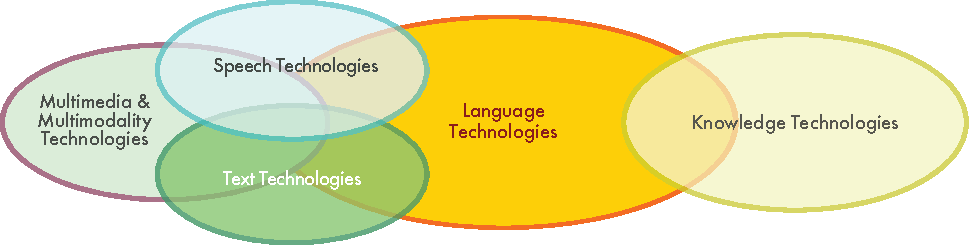
\includegraphics[width=\textwidth]{../_media/english/language_technologies}
  \caption{Language technology in context}
  \label{fig:ltincontext_en}
  \colorrule{grey3}{\textwidth}{1.5pt}
\end{figure*}

When we communicate, we combine language with other modes of communication and information media --~for example speaking can involve gestures and facial expressions. Digital texts link to pictures and sounds. Movies may contain language in spoken and written form. In other words, speech and text technologies overlap and interact with other multimodal communication and multimedia technologies.\\ 
In this section, we will discuss the main application areas of language technology, i.\,e., language checking, web search, speech interaction, and machine translation. These applications and basic technologies include 

\begin{itemize}
\item spelling correction
\item authoring support
\item computer-assisted language learning
\item information retrieval 
\item information extraction
\item text summarisation
\item question answering
\item speech recognition 
\item speech synthesis 
\end{itemize}

Language technology is an established area of research with an extensive set of introductory literature. The interested reader is referred to the following references:  \cite{Braasch, jurafsky-martin01, manning-schuetze1, lt-world1, lt-survey1}.

Before discussing the above application areas, we will briefly describe the architecture of a typical LT system.

\subsection{Application Architectures}

\begin{figure*}[b]
  \colorrule{grey3}{\textwidth}{1.5pt}
  \center
  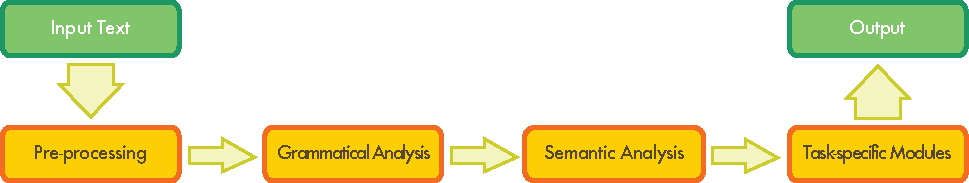
\includegraphics[width=\textwidth]{../_media/english/text_processing_app_architecture}
  \caption{A typical text processing architecture}
  \label{fig:textprocessingarch_en}
  \colorrule{grey3}{\textwidth}{1.5pt}
\end{figure*}

Software applications for language processing typically consist of several components that mirror different aspects of language. While such applications tend to be very complex, figure~\ref{fig:textprocessingarch_en} shows a highly simplified architecture of a typical text processing system. The first three modules handle the structure and meaning of the text input:

\begin{enumerate}
\item Pre-processing: cleans the data, analyses or removes formatting, detects the input languages, and so on.
\item Grammatical analysis: finds the verb, its objects, modifiers and other sentence elements; detects the sentence structure.
\item Semantic analysis: performs disambiguation (i.\,e., computes the appropriate meaning of words in a given context); resolves anaphora (i.\,e., which pronouns refer to which nouns); represents the meaning of the sentence in a machine-readable way.
\end{enumerate}

After analysing the text, task-specific modules can perform other operations, such as automatic summarisation and database look-ups.

In the remainder of this section, we firstly introduce the core application areas for language technology, and follow this with a brief overview of the state of LT research and education today, and a description of past and present research programmes. Finally, we present an expert estimate of core LT tools and resources for Danish in terms of various dimensions such as availability, maturity and quality. The general situation of LT for the Danish language is summarised in a matrix (figure~\ref{fig:lrlttable_en}, p.~\pageref{fig:lrlttable_en}) at the end of this chapter. Tools and resources that are boldfaced in the text can also be found in figure~\ref{fig:lrlttable_en}. LT support for Danish is also compared to other languages that are part of this series.

\subsection{Core Application Areas}

In this section, we focus on the most important LT tools and resources, and provide an overview of LT activities in Denmark. 

\subsubsection{Language Checking}

\begin{figure*}[th]
  \colorrule{grey3}{\textwidth}{1.5pt}
  \center
  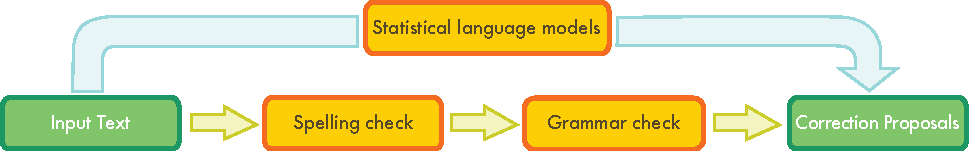
\includegraphics[width=\textwidth]{../_media/english/language_checking}
  \caption{Language checking (statistical; rule-based)}
  \label{fig:langcheckingaarch_en}
  \colorrule{grey3}{\textwidth}{1.5pt}
\end{figure*}

Anyone who has used a word processor such as Microsoft Word knows that it has a spell checker that highlights spelling mistakes and proposes corrections. The first spelling correction programs compared a list of extracted words against a dictionary of correctly spelled words. Today these programs are far more sophisticated. Using language-dependent algorithms for \textbf{grammatical analysis}, they detect errors related to morphology (e.\,g., plural formation) as well as syntax–related errors, such as a missing verb or a conflict of verb-subject agreement (e.\,g., \textit{she *write a letter}). However, most spell checkers will not find any errors in the following text \cite{zar1}:

\begin{quote}
  {\it I have a spelling checker,\\
  It came with my PC.\\
  It plane lee marks four my revue\\
  Miss steaks aye can knot sea.}
\end{quote}

Handling these kinds of errors usually requires an analysis of the context. 
This type of analysis either needs to draw on language-specific \textbf{grammars} laboriously coded into the software by experts, or on a statistical language model. In this case, a model calculates the probability of a particular word as it occurs in a specific position (e.\,g., between the words that precede and follow it). For example: \textit{stort hus} [big house] is a much more probable word sequence than \textit{stor hus} [big house]. A statistical language model can be automatically created by using a large amount of (correct) language data, a \textbf{text corpus}. Most of these two approaches have been developed around data from English. Neither approach can transfer easily to Danish because the language has unlimited compound building and a richer inflection system.

Thus, a serious defect of early stage Danish spell checkers was the incorrect markings of productive compounds, for instance, {\it pasningsordning} [childcare arrangement]. If these were not lexicalised in dictionaries or word lists (where the productive ones are generally not), they resulted in an error marking. Such wrong markings appeared due to lack of high-quality compound splitters for Danish that could check each component of the compound per se. Unfortunately, this flaw in early stage spell checkers for Danish has lead to an increase in spelling errors. People are influenced partly by the split compound tendency in English, and partly by the fact that a split compound does not result in an error marking with a Danish spell checker. Recent spell checkers for Danish as provided for instance by Microsoft Office products have now improved with regards to this phenomenon. 

Danish grammar checkers, however, are still at a rather initial level. They are generally able to identify some simple grammatical errors such as lack of short dependency concordance as in {\it *den r\o de hus} [red house; wrong gender of {\it den} and {\it red}], whereas other grammatical errors are not identified, such as {\it *jeg var kede af at du ikke kom} [I was sorry that you didn't come; wrong number on {\it ked} [sorry]]. 

Recently, also OpenOffice provides Danish language checking tools to a certain extent. Magenta  has integrated several open source Danish lexical resources into the document processing tool, including writing aids such as synonymy look-up. 

Specifically related to teaching, Mikro V\ae rk\-stedet is one of the prime players in the market for digital teaching facilities, including reading tools for dyslexia clients as well as writing aids. Further, Ordbogen.com should be mentioned for facilitating the use of online dictionaries.  

Language checking is not limited to word processors; it is also used in “authoring support systems”, i.\,e., software environments in which manuals and other types of technical documentation for complex IT, healthcare, engineering and other products, are written. To offset customer complaints about incorrect use and damage claims resulting from poorly understood instructions, companies are increasingly focusing on the quality of technical documentation while targeting the international market (via translation or localisation) at the same time. Advances in natural language processing have led to the development of authoring support software, which helps the writer of technical documentation to use vocabulary and sentence structures that are consistent with industry rules and (corporate) terminology restrictions.

\boxtext{Language checking is not limited to word processors but also applies to authoring systems.}

Besides spell checkers and authoring support, language checking is also important in the field of computer-assisted language learning. Language checking applications also automatically correct search engine queries, as found in Google's \textit{Did you mean…} suggestions.

\subsubsection{Web Search}

\begin{figure*}[htb]
  \colorrule{grey3}{\textwidth}{1.5pt}
  \center
  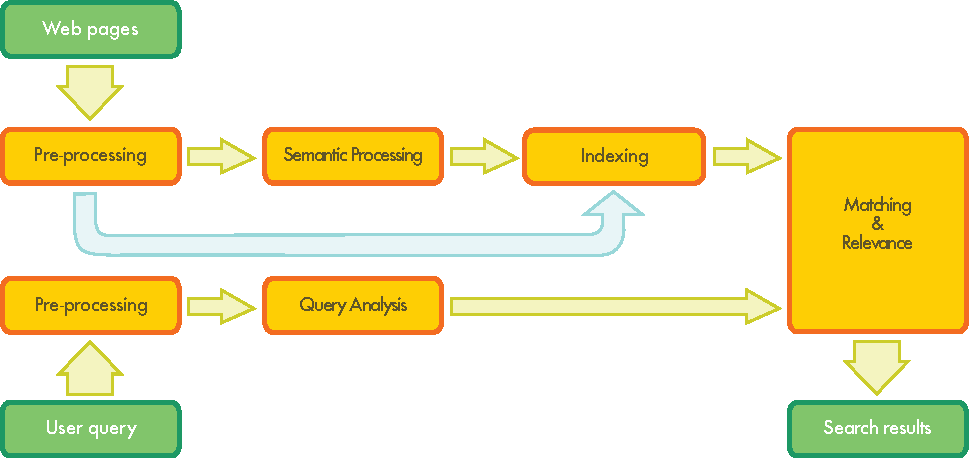
\includegraphics[width=\textwidth]{../_media/english/web_search_architecture}
  \caption{Web search}
  \label{fig:websearcharch_en}
  \colorrule{grey3}{\textwidth}{1.5pt}
 \end{figure*}

Searching the Web, intranets or digital libraries is probably the most widely used yet largely underdeveloped language technology application today. The Google search engine, which started in 1998, now handles about 80\% of all search queries \cite{spi1}. The verb {\it google} even has an entry in the Danish dictionary `Den Danske Ordbog'. The Google search interface and results page display has not significantly changed since the first version. However, in the current version, Google offers spelling correction for misspelled words and incorporates basic semantic search capabilities that can improve search accuracy by analysing the meaning of terms in a search query context \cite{pc1}. The Google success story shows that a large volume of data and efficient indexing techniques can deliver satisfactory results using a statistical approach to language processing. 

For more sophisticated information requests, it is essential to integrate deeper linguistic knowledge to facilitate text interpretation. Experiments using \textbf{lexical resources} such as machine-readable thesauri or ontological language resources (e.\,g., WordNet for English or DanNet for Danish) have demonstrated improvements in finding pages using synonyms of the original search terms, such as \textit{autoforsikring} {[}auto insurance{]}, \textit{bilforsikring} {[}motor car insurance{]} and \textit{kaskoforsikring} {[}insurance covering loss of or damage to the car{]}, or even more loosely related terms.

\boxtext{The next generation of search engines will have to include much more sophisticated language technology.}

The next generation of search engines will have to include much more sophisticated language technology, especially to deal with search queries consisting of a question or other sentence type rather than a list of keywords. For the query, \textit{Give me a list of all companies that were taken over by other companies in the last five years}, a syntactic as well as \textbf{semantic analysis} is required. The system also needs to provide an index to quickly retrieve relevant documents. A satisfactory answer will require syntactic parsing to analyse the grammatical structure of the sentence and determine that the user wants companies that have been acquired, rather than companies that have acquired other companies. For the expression \textit{last five years}, the system needs to determine the relevant range of years, taking into account the present year. The query then needs to be matched against a huge amount of unstructured data to find the pieces of information that are relevant to the user’s request. This process is called information retrieval, and involves searching and ranking relevant documents. To generate a list of companies, the system also needs to recognise a particular string of words in a document represents a company name, using a process called ``named entity recognition''.

A more demanding challenge is matching a query in one language with documents in another language. Cross-lingual information retrieval involves automatically translating the query into all possible source languages and then translating the results back into the user's target language.

Now that data is increasingly found in non-textual formats, there is a need for services that deliver multimedia information retrieval by searching images, audio files and video data. In the case of audio and video files, a speech recognition module must convert the speech content into text (or into a phonetic representation) that can then be matched against a user query.

In Denmark, SMEs like Ankiro, ScanJour, LAT Consulting, Findwise, RDFined and others successfully develop and apply search technologies that are tailored to specific company needs.

These companies focus their development on providing add-ons and advanced search engines for special interest portals by using topic-relevant semantics. Due to the constant high demand for processing power, such search engines are only cost-effective when handling relatively small text corpora. The processing time is several thousand times higher than that needed by a standard statistical search engine, like Google. These search engines are in high demand for topic-specific domain modelling, but they cannot be used on the Web with its billions and billions of documents. Furthermore, the technologies developed in these contexts are generally not available to the public for further research or development. Due to such practical obstacles, many Danish websites link to a Google search engine as their only search facility.

Experimental, ontology-based search engines have been developed at several Danish universities such as Roskilde Universitet. The OntoQuery and SIABO prototypes are examples of such experimental search engines that work on smaller domains with a rich ontological representation.  Again, however, such prototypes are not easily scalable to larger domains.

\subsubsection{Speech Interaction}

Speech interaction is one of many application areas that depend on speech technology, i.\,e., technologies for processing spoken language. Speech interaction technology is used to create interfaces that enable users to interact in spoken language instead of using a graphical display, keyboard and mouse.  Today, these voice user interfaces (VUI) are used for partially or fully automated telephone services provided by companies to customers, employees or partners. Business domains that rely heavily on VUIs include banking, supply chain, public transportation, and telecommunications. Other uses of speech interaction technology include interfaces to car navigation systems and the use of spoken language as an alternative to the graphical or touchscreen interfaces in smartphones.

\begin{figure*}[htb]
  \colorrule{grey3}{\textwidth}{1.5pt}
  \center
  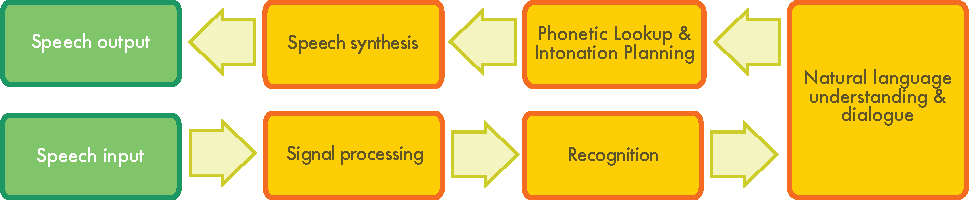
\includegraphics[width=\textwidth]{../_media/english/simple_speech-based_dialogue_architecture}
  \caption{Speech-based dialogue system}
  \label{fig:dialoguearch_en}
  \colorrule{grey3}{\textwidth}{1.5pt}
\end{figure*}

Speech interaction technology comprises four technologies: 

\begin{enumerate}
\item Automatic \textbf{speech recognition} (ASR) determines which words are actually spoken in a given sequence of sounds uttered by a user.  
\item Natural language understanding analyses the syntactic structure of a user’s utterance and interprets it according to the system in question.
\item Dialogue management determines which action to take given the user input and system functionality.   
\item \textbf{Speech synthesis} (text-to-speech or TTS) trans\-forms the system’s reply into sounds for the user.
\end{enumerate}

One of the major challenges of ASR systems is to accurately recognise the words a user utters. This means restricting the range of possible user utterances to a limited set of keywords, or manually creating language models that cover a large range of natural language utterances. Using machine learning techniques, language models can also be generated automatically from \textbf{speech corpora}, i.\,e., large collections of speech audio files and text transcriptions. Restricting utterances usually forces people to use the voice user interface in a rigid way and can damage user acceptance; but the creation, tuning and maintenance of rich language models will significantly increase costs. VUIs that employ language models and initially allow a user to express their intent more flexibly --~prompted by a \textit{How may I help you?} greeting~-- tend to be automated and are better accepted by users.

\boxtext{Speech interaction is the basis for interfaces that allow a user to interact with spoken language.}

Companies tend to use utterances pre-recorded by professional speakers for generating the output of the voice user interface. For static utterances where the wording does not depend on particular contexts of use or personal user data, this can deliver a rich user experience. But more dynamic content in an utterance may suffer from unnatural intonation because different parts of audio files have simply been strung together. Through optimisation, today’s TTS systems are getting better at producing natural-sounding dynamic utterances.

Interfaces in speech interaction have been considerably standardised during the last decade in terms of their various technological components. There has also been strong market consolidation in speech recognition and speech synthesis. The national markets in the G20 countries (economically resilient countries with high populations) have been dominated by just five global players, with Nuance (USA) and Loquendo (Italy) being the most prominent players in Europe. In 2011, Nuance announced the acquisition of Loquendo, which represents a further step in market consolidation.

On the Danish market for speech technology solutions there are a
number of national companies (Mikro V\ae rkstedet, Prolog Development
Center, Max Manus, as well as IBM and Siemens Denmark) that have
specialised in providing speech-based solutions powered by technology
developed by the leading international technology suppliers. Nuance is
the predominant international speech technology provider of Danish
speech technology. Virtually all other providers of Danish speech
technology have been acquired by Nuance over the last 5-6 years, for
example, Philips Speech Magic, Loquendo and SVOX.

Currently there are two software packages that offer Danish speech
recognition, Nuance SpeechMagic and Nuance Dragon Development Platform
(cloud-based). Based on these technologies Max Manus has developed an
application for the health care sector, IBM an application for the
municipal sector and Prolog Development Center the standard system
Dictus and customised solutions for Folketingstidende (The Parliament
Hansard) and two national broadcasters. Nuance developed the free Apps
Dragon Dictation and Dragon Search for the iPhone/iPad while Prolog
Development Center delivers Dictus to Android on the same cloud-based
platform. Nuance is the only supplier of speech recognition telephone
technology. Siemens Denmark and Prolog Development Center are the
Danish companies that have supplied voice-controlled telephone service
on the basis of Nuance Recognizer v9. 
Currently there are more than 10 different Danish voices for speech
synthesis developed by Nuance (including Loquendo and SVOX), Acapela,
and the Danish company Mikro V\ae rkstedet. The successful Polish
company IVONA is also planning to launch a number of Danish voices in
early 2012.

A growing number of major international suppliers of consumer
electronics (Garmin, Navigon, Samsung) offer products that incorporate
Danish speech recognition so that the products can be controlled by
voice. An even larger number of products, such as iRobot, have also
built-in Danish speech synthesis. A small but growing number of Danish
producers of consumer products utilise Danish speech technology, for
example, 6th Sense Solution for reading bus stops and CIM Interconn
for screen reading in nursing homes.

The demand for voice user interfaces in Denmark has grown fast in the last five years, driven by increasing demand for customer self-service, cost optimisation for automated telephone services, and the increasing acceptance of spoken language as a media for human-machine interaction. 

Looking ahead, there will be significant changes, due to the spread of smartphones as a new platform for managing customer relationships, in addition to fixed telephones, the Internet and e-mail. This will also affect how speech interaction technology is used. In the long term, there will be fewer telephone-based VUIs, and spoken language apps will play a far more central role as a user-friendly input for smartphones. This will be largely driven by stepwise improvements in the accuracy of speaker-independent speech recognition via the speech dictation services already offered as centralised services to smartphone users.

\subsubsection{Machine Translation}

\begin{figure*}[htb]
  \colorrule{grey3}{\textwidth}{1.5pt}
  \center
  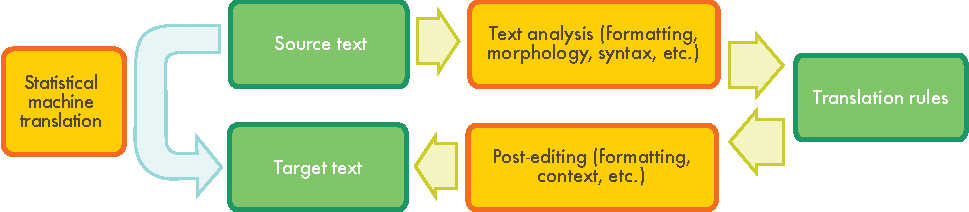
\includegraphics[width=\textwidth]{../_media/english/machine_translation}
  \caption{Machine translation (statistical; rule-based)}
  \label{fig:mtarch_en}
  \colorrule{grey3}{\textwidth}{1.5pt}
\end{figure*}

The idea of using digital computers to translate natural languages can be traced back to 1946 and was followed by substantial funding for research during the 1950s and again in the 1980s. 
Yet \textbf{machine translation} (MT) still cannot deliver on its initial promise of providing across-the-board automated translation.  

\boxtext{At its basic level, Machine Translation simply substitutes words in one natural language with words in another language.}

The most basic approach to machine translation is the automatic replacement of the words in a text written in one natural language with the equivalent words of another language. This can be useful in subject domains that have a very restricted, formulaic language such as weather reports.
However, in order to produce a good translation of less restricted texts, larger text units (phrases, sentences, or even whole passages) need to be matched to their closest counterparts in the target language. The major difficulty is that human language is ambiguous. Ambiguity creates challenges on multiple levels, such as word sense disambiguation at the lexical level (a \textit{jaguar} is a brand of car or an animal) or the assignment of case on the syntactic level, for example:

\begin{itemize}
\item {\it The woman saw the car and her husband, too.}
\end{itemize}

One way to build an MT system is to use linguistic rules. For translations between closely related languages, a translation using direct substitution may be feasible in cases such as the above example. However, rule-based (or linguistic knowledge-driven) systems often analyse the input text and create an intermediary symbolic representation from which the target language text can be generated. The success of these methods is highly dependent on the availability of extensive lexicons with morphological, syntactic, and semantic information, and large sets of grammar rules carefully designed by skilled linguists. This is a very long and therefore costly process.

In the late 1980s when computational power increased and became cheaper, interest in statistical models for machine translation began to grow. Statistical models are derived from analysing bilingual text corpora, \textbf{parallel corpora}, such as the Europarl parallel corpus, which contains the proceedings of the European Parliament in 21 European languages. Given enough data, statistical MT works well enough to derive an approximate meaning of a foreign language text by processing parallel versions and finding plausible patterns of words. Unlike knowledge-driven systems, however, statistical (or data-driven) MT systems often generate ungrammatical output. Data-driven MT is advantageous because less human effort is required, and it can also cover special particularities of the language (e.\,g., idiomatic expressions) that are often ignored in knowledge-driven systems. 

\boxtext{Machine Translation is particularly challenging for the Danish language.}

The strengths and weaknesses of knowledge-driven and data-driven machine translation tend to be complementary, so that nowadays researchers focus on hybrid approaches that combine both methodologies. One such approach uses both knowledge-driven and data-driven systems, together with a selection module that decides on the best output for each sentence. However, results for sentences longer than, say, 12 words, will often be far from perfect. A more effective solution is to combine the best parts of each sentence from multiple outputs; this can be fairly complex, as corresponding parts of multiple alternatives are not always obvious and need to be aligned. 

The potential for creating arbitrary new words by compounding makes dictionary analysis and dictionary coverage difficult; split verb constructions pose problems for analysis; and extensive lexical ambiguity is a challenge for word sense disambiguation.
Apart from the PaTrans system (a patent translation system for English-Danish) early MT systems for Danish, like the SYSTRAN prototype, were primarily developed by foreign companies.
All of these systems are rule-based. Although significant research in this technology exists in national and international contexts, this situation has not substantially changed, even if there are some Danish start-ups such as Grammar Soft and Languagelens, providing rule-based and statistical machine translation systems for Danish. A majority of the available systems, like, e.\,g., Google Translate and ESTeam Translator, is still developed abroad.

There is still a huge potential for improving the quality of MT systems. The challenges involve adapting language resources to a given subject domain or user area, and integrating the technology into workflows that already have term bases and translation memories. Another problem is that most of the current systems are English-centred and only support a few languages from and into Danish. This leads to friction in the translation workflow and forces MT users to learn different lexicon coding tools for different systems.

Evaluation campaigns help to compare the quality of MT systems, the different approaches and the status of the systems for different language pairs. Figure~\ref{fig:euromatrix_de} (p.~\pageref{fig:euromatrix_de}), which was prepared during the EC Euromatrix+ project, shows the pair-wise performances obtained for 22 of the 23 official EU languages (Irish was not compared). The results are ranked according to a BLEU score, which indicates higher scores for better translations \cite{bleu1}. A human translator would normally achieve a score of around 80 points.

The best results (in green and blue) were achieved by languages that benefit from a considerable research effort in coordinated programmes and the existence of many parallel corpora (e.\,g., English, French, Dutch, Spanish and German). The languages with poorer results are shown in red. These languages either lack such development efforts or are structurally very different from other languages (e.\,g., Hungarian, Maltese and Finnish).


\subsection{Other Application Areas}

Building language technology applications involves a range of subtasks that do not always surface at the level of interaction with the user, but they provide significant service functionalities “behind the scenes” of the system in question. They all form important research issues that have now evolved into individual sub-disciplines of computational linguistics.  Question answering, for example, is an active area of research for which annotated corpora have been built and scientific competitions have been initiated. The concept of question answering goes beyond keyword-based searches (in which the search engine responds by delivering a collection of potentially relevant documents) and enables users to ask a concrete question to which the system provides a single answer. For example:

\begin{itemize}
\item[] \textit{Question: How old was Neil Armstrong when he stepped on the moon?}
\item[] \textit{Answer: 38.}
\end{itemize}

While question answering is obviously related to the core area of web search, it is nowadays an umbrella term for such research issues as which different types of questions exist, and how they should be handled; how a set of documents that potentially contain the answer can be analysed and compared (do they provide conflicting answers?); and how specific information (the answer) can be reliably extracted from a document without ignoring the context. 

\boxtext{Language technology applications often provide significant service functionalities behind the scenes of larger software systems.}

Question answering is in turn related to information extraction (IE), an area that was extremely popular and influential when computational linguistics took a statistical turn in the early 1990s. IE aims to identify specific pieces of information in specific classes of documents, such as the key players in company takeovers as reported in newspaper stories. Another common scenario that has been studied is reports on terrorist incidents. The task here consists of mapping appropriate parts of the text to a template that specifies the perpetrator, target, time, location and results of the incident. Domain-specific template-filling is the central characteristic of IE, which makes it another example of a “behind the scenes” technology that forms a well-demarcated research area, which in practice needs to be embedded into a suitable application environment. 

    Text summarisation and \textbf{text generation} are two borderline areas that can act either as standalone applications or play a supporting role. Summarisation attempts to give the essentials of a long text in a short form, and is one of the features available in Microsoft Word. It mostly uses a statistical approach to identify the “important” words in a text (i.\,e., words that occur very frequently in the text in question but less frequently in general language use) and determine which sentences contain the most of these “important” words. These sentences are then extracted and put together to create the summary. In this very common commercial scenario, summarisation is simply a form of sentence extraction, and the text is reduced to a subset of its sentences. An alternative approach, for which some research has been carried out, is to generate brand new sentences that do not exist in the source text. 

\boxtext{For the Danish language, research in most text technologies is much less developed than for the English language.}

This requires a deeper understanding of the text, which means that so far this approach is far less robust. On the whole, a text generator is rarely used as a stand-alone application but is embedded into a larger software environment, such as a clinical information system that collects, stores and processes patient data. Creating reports is just one of many applications for text summarisation. 
For the Danish language, research in these text technologies is much less developed than for the Eng\-lish language. Question answering, information extraction, and summarisation have been the focus of numerous open competitions in the USA since the 1990s, primarily organised by the government-sponsored organisations DARPA and NIST. These competitions have significantly improved the state of the art, but their focus has mostly been on the English language. As a result, there are hardly any annotated corpora or other special resources for these tasks in Danish. 

Some Danish SMEs (such as RDFined and Ankiro) and media (Information, InfoMedia, DR) 
are engaged in small, task-driven initiatives on named entity recognition and knowledge extraction.  Some of these draw on tools developed at the Centre for Language Technology at the University of Copenhagen: part of speech tagger, lemmatiser, keyword extractor.  Some apply the computational dictionary STO, and/or the Danish wordnet (DanNet), which are resources that have been developed in collaboration with other institutions. Likewise a summarisation system, DanSum, is available online at the Centre's website.  For text generation, reusable components have traditionally been limited to the surface realisation modules (the “generation grammar”); again, most available software is for English. 


\subsection{Language Technology in Research and Education}

  Language technology research is performed at several research institutions in Denmark and through several collaborative infrastructure and research projects. In the following, only prime movers in the field as well as currently ongoing projects are listed, acknowledging the fact that related research takes place also at other institutions and in other projects than the ones mentioned here.

As previously mentioned, Centre for Language Technology at the University of Copenhagen is the national centre for language technology.  The Centre's main research topics are language resources and tools such as LSP corpora and wordnets, multilinguality (machine translation, controlled language etc.), multimodality, information retrieval, use of ontologies and incorporation of language technology in other application areas, as for example e-learning.

The Department of International Language Studies and Computational Linguistics, Copenhagen Business School, performs research in text technology and computational linguistics including tree\-banks, statistical machine translation, terminology and speech technology. Taking their point of departure in language, text and translation studies, researchers at the department  in general focus on how companies can deal with their language processes professionally in a globalised world and on issues related to language for special purposes (LSP). Copenhagen Business School includes the DANTERMcentre which is a centre for terminology and development of terminology tools.

At the Institute of Language and Communication, University of Southern Denmark, several researchers work within the field of language technology and computational linguistics, for instance within the VISL project (Visual Interactive Syntax Learning). Aalborg University, Department of Electronic Systems, is a prime mover in research regarding speech technology. The Danish Language Council as well as the Society for Danish Language and Literature are also engaged in language technology-related research, especially with regard to the development of dictionaries and corpora and the corpus-based identification of new words in Danish. 

Several research infrastructure projects are ongoing in Denmark, such as DK-CLARIN, which has the aim to construct a Danish research infrastructure for the humanities integrating written, spoken, and visual records into a coherent and systematic digital repository. Moreover, LARM has the aim of constructing a national, digital and user-driven research infrastructure, which will provide a solution for preserving and maturing cultural heritage radio source material. 

There are also several collaborative research projects such as ESICT, NOMCO and DanTermBank. ESICT performs research in methods and development of technologies providing citizens with an innovative information system on health and disease, based on information technology, language technology and formalised medical knowledge. NOMCO is a Nordic collaborative project which deals with multimodal corpus analysis. DanTermBank is a recently initiated project concerned with the development of the technological foundations for national term bank for languages for special purposes. Furthermore, Danish research centers participate in several ongoing European projects related to language technology, LetsMT!, CLARIN, CLARA, META-NORD/META-NET  to mention a few.

In contrast to the relatively high-level research activity in language technology in Denmark, the educational situation can only be labeled as critical. Currently, there exists no bachelor's or master's degree in language technology in Denmark. Language technology is only taught as a component of other bachelor's and master's educations in Denmark. Examples are the master's program in {\it IT and Cognition} at the University of Copenhagen, which encompasses an obligatory course in language technology, as well as the bachelor's program in {\it Business Communication and IT} at the University of Southern Denmark, which includes an optional branch of language technology. The lack of education in basic language technology is problematic and constitutes a rather new situation in the country, since computational linguistics was taught until recently both at the Copenhagen Business School and the University of Copenhagen. The current situation should encourage political actions since future research and development of Danish language technology may be in danger. Paradoxically, the lack of education in the field coincides with an increasing interest in and demand for language technology in Danish industry. 

\subsection{National Projects and Initiatives}

 The Danish research councils have supported language technology projects over the years, and in the past also created specific research programmes supporting the field.

The European EUROTRA programme was probably the first large scale support for language technology in Denmark. The EUROTRA effort aimed at creating multilingual machine translation for all official European languages. It started late 1970s and ran till early 1990s. A Dane was chairing the EUROTRA Liaison Group 1986-1992, which brought some attention to the project from Danish players. Although EUROTRA did not produce a ready to use multilingual machine translation system, it did provide a prototype and thereby the necessary background for a patent machine translation system for English-Danish, running in production for more than 10 years.

One of the early programmes created by the Research Council for the Humanities was ETTO ({\it Edb for Tekst, Tale og Ordb\o ger} [Computing for Text, Speech and Dictionaries]) 1982-85. The next programme was {\it Eksperimentel Sprogvidenskab} [Experimental linguistics]) running from 1991. Since then, the Research Council for Humanities has not had specific programmes aiming at language technology.

The Research Council for the Technical Sciences had speech technology as one of the main themes in their strategy plan for 1998-2002, and they did support several language technology projects.

The inter-disciplinary IT research programmes running from mid 1990s to 2003 have been able to support a few language technology related projects (as was the case for OntoQuery and SIABO), but have not had a specific aim to do so.

The Research Agency of the Danish Ministry for Science, Technology and Development decided in 2001 to promote language technology by funding a collaborative effort to enlarge the Danish language technology lexicon developed in the European PAROLE project. The resulting dictionary (STO) is now available through ELRA, and is being used for research and commercial purposes. It was the specific aim of the Research Agency to support the Danish language in the digital age, by granting funds for the development of basic language technology building blocks.

Since this funding, to our knowledge there have been no programmes for the support of language technology specifically, but as always, language technology projects may be supported by research councils etc. in competition with other themes.

In parallel with the ESFRI initiative for research infrastructure, Denmark has started a roadmap process for research infrastructures. One of the research infrastructures to be supported will be a “Digital Humanities Laboratory” for the support of humanities research through the use of i.a. language technology.


As we have seen, previous programmes have led to the development of a number of LT tools and resources for the Danish language. The following section summarises the current state of LT support for Danish.
  
\subsection{Availability of Tools and Resources}

Figure~\ref{fig:lrlttable_en} provides a rating for language technology support for the Danish language. This rating of existing tools and resources was generated by leading experts in the field who provided estimates based on a scale from 0 (very low) to 6 (very high) using seven criteria.

\begin{figure*}[htb]
\centering
%\begin{tabular}{>{\columncolor{orange1}}p{.33\linewidth}ccccccc} % ORIGINAL
\begin{tabular}{>{\columncolor{orange1}}p{.33\linewidth}@{\hspace*{6mm}}c@{\hspace*{6mm}}c@{\hspace*{6mm}}c@{\hspace*{6mm}}c@{\hspace*{6mm}}c@{\hspace*{6mm}}c@{\hspace*{6mm}}c}
\rowcolor{orange1}
 \cellcolor{white}&\begin{sideways}\makecell[l]{Quantity}\end{sideways}
&\begin{sideways}\makecell[l]{\makecell[l]{Availability} }\end{sideways} &\begin{sideways}\makecell[l]{Quality}\end{sideways}
&\begin{sideways}\makecell[l]{Coverage}\end{sideways} &\begin{sideways}\makecell[l]{Maturity}\end{sideways} &\begin{sideways}\makecell[l]{Sustainability~~~}\end{sideways} &\begin{sideways}\makecell[l]{Adaptability}\end{sideways} \\ \addlinespace
\multicolumn{8}{>{\columncolor{orange2}}l}{Language Technology: Tools, Technologies and Applications} \\ \addlinespace
Speech Recognition	&4&2&--*&4&4&3&3 \\ \addlinespace
Speech Synthesis &5&2&--*&3&3&2&3\\ \addlinespace
Grammatical analysis &3&2&4&4&3&2&3\\ \addlinespace
Semantic analysis &1&0&1&1&1&1&1\\ \addlinespace
Text generation &0&0&0&0&0&0&0\\ \addlinespace
Machine translation &3&2&2&3&3&1&2\\ \addlinespace
\multicolumn{8}{>{\columncolor{orange2}}l}{Language Resources: Resources, Data and Knowledge Bases} \\ \addlinespace
Text corpora &4&3&4&3&4&4&3\\ \addlinespace
Speech corpora &3&3&3&1&2&2&2\\ \addlinespace
Parallel corpora &3&1&3&2&2&2&2\\ \addlinespace
Lexical resources &3&3&4&4&3&3&3\\ \addlinespace
Grammars &2&1&4&1&2&2&2\\
\end{tabular}
\caption{State of language technology support for Danish (*quality has not been rated; see explanation in the text)}
\label{fig:lrlttable_en}
\end{figure*}

The key results for Danish language technology can be summed up as follows:

\begin{itemize}
\item In speech technology, there exist some tools, but almost exclusively available on a commercial basis. Regarding their quality however, commercial developers and researchers disagree. Where commercial developers argue that the recognition rate is at least 95\%, the researchers point out that this high recognition rate can only be achieved if the speaker speaks very clearly and the system knows the user's voice in advance. Due to this disagreement, quality has not been rated in figure~\ref{fig:lrlttable_en}.
\item With respect to basic text analysis the situation in Denmark is reasonably good. There exist a couple of tokenisers, part of speech taggers and morphological analysers of relatively high quality and broad coverage.  However, not all of them are freely available. Broad coverage syntactic parsers on the other hand are sparse even if work has been done on constraint grammars and dependency parsing.
\item Semantics is more difficult to process than syntax, and text semantics is more difficult to process than word and sentence semantics. Semantic tools and resources are scored very low. 
%Thus, programs and initiatives are needed to substantially boost this area both with regard to basic research %and the development of annotated corpora.
\item There is substantial research going on in the field of machine translation at several Danish research institutions, in particular on statistical machine translation. However, the quality is still low, and the number of language pairs is limited.
\item With regard to resources such as reference corpora, lexicons, wordnets and terminologies, the situation is also reasonably good for Danish since substantial resources have been built in recent years; however, IPR issues prevent that all corpora become freely available. While some reference corpora of high quality exist, large syntactically and semantically annotated corpora are not available. For multimodal corpora, some annotated corpora are under development, but not yet available. There is a lack of parallel corpora needed for statistical and hybrid approaches to machine translation.
\item Several of the resources lack standardisation, i.\,e., even if they exist, sustainability is not given.
\end{itemize}

In a number of specific areas of Danish language research, we have software with limited functionality available today. Obviously, further research efforts are required to meet the current deficit in processing texts on a deeper semantic level and to address the lack of resources such as parallel corpora for machine translation.  Concerted programs and initiatives are needed to standardise data and interchange formats.

\subsection{Cross-language comparison}

The current state of LT support varies considerably from one language
community to another. In order to compare the situation between
languages, this section will present an evaluation based on two sample
application areas (machine translation and speech processing) and one
underlying technology (text analysis), as well as basic resources
needed for building LT applications. The languages were categorised
using a five-point scale: 

\begin{enumerate}
\item Excellent support
\item Good support
\item Moderate support
\item Fragmentary support
\item Weak or no support
\end{enumerate}

LT support was measured according to the following criteria:

\textbf{Speech Processing:} Quality of existing speech recognition technologies, quality of existing speech synthesis technologies, coverage of domains, number and size of existing speech corpora, amount and variety of available speech-based applications.

\textbf{Machine Translation:} Quality of existing MT technologies, number of language pairs covered, coverage of linguistic phenomena and domains, quality and size of existing parallel corpora, amount and variety of available MT applications.

\textbf{Text Analysis:} Quality and coverage of existing text analysis technologies (morphology, syntax, semantics), coverage of linguistic phenomena and domains, amount and variety of available applications, quality and size of existing (annotated) text corpora, quality and coverage of existing lexical resources (e.\,g., WordNet) and grammars.

\textbf{Resources:} Quality and size of existing text corpora, speech corpora and parallel corpora, quality and coverage of existing lexical resources and grammars.

Figures~\ref{fig:speech_cluster_en} to~\ref{fig:resources_cluster_en} show that Denmark is roughly estimated to be at the same level as its Scandinavian neighbors (Sweden, Norway and Finland). However,  Denmark is in the second-worst category for speech processing (although, as mentioned above, there is some disagreement among researchers and commercial developers about the quality), text analysis and resources.
 The figures are even lower im machine translation. Here, Denmark is in the worst category, along with many other countries.

 Thus, for building more sophisticated applications, such as machine translation, there is a clear need for resources and technologies that cover a wider range of linguistic aspects and enable a deep semantic analysis of the input text. By improving the quality and coverage of these basic resources and technologies, we shall be able to open up new opportunities for tackling a broader range of advanced application areas, including high-quality machine translation.

\subsection{Conclusions}

\emph{In this series of white papers, we have made an important effort by assessing the language technology support for 30 European languages, and by providing a high-level comparison across these languages. By identifying the gaps, needs and deficits, the European language technology community and its related stakeholders are now in a position to design a large scale research and development programme aimed at building a truly multilingual, technology-enabled communication across Europe.}

The results of this white paper series show that there is a dramatic difference in language technology support between the various European languages. While there are good quality software and resources available for some languages and application areas, others, usually smaller languages, have substantial gaps. Many languages lack basic technologies for text analysis and the essential resources. Others have basic tools and resources but the implementation of, for example semantic methods, is still far away. Therefore a large-scale effort is needed to attain the ambitious goal of providing high-quality language technology support for all European languages, for example through high quality machine translation. 

For Danish, the results indicate that only with respect to the most basic tools and resources the situation is reasonably good. Furthermore, there exist some systems for information extraction, machine translation and speech recognition and synthesis, as well as resources like parallel corpora, and speech corpora. However, these systems and resources are rather simple and have a limited functionality for some of the areas. For instance, parallel corpora only exist for very few language pairs.

With respect to more advanced fields like sentence and text semantics, information retrieval, language generation, and annotated multimodal data, Danish clearly lacks systems, tools and resources even if some of these are currently under development. For advanced semantic and discourse processing and  dialogue management resources are very scarce and systems have a quite limited scope.

Another point which is not fully reflected in the table above is that language technology resources and tools for Danish alone do not necessarily facilitate globalisation and international cooperation. ``Cross- and multilingual'' technologies that link Danish to other languages (for instance machine translation, multilingual retrieval, parallel corpora, linked wordnets, etc.) are a prerequisite for high-level, technology-aided interaction with our surroundings. 

Given the present situation and the importance of language technology as the key for protecting and furthering the Danish language in the information-driven society, these results indicate that there is an indispensable need for new programmes specifically focusing on the development of language technology systems, tools and resources. In contrast to several other Nordic countries which have, for example,  initiated projects concerning the development of a language bank encompassing a set of basic resources and tools (a BLARK), recent research and development in Denmark has been performed in full competition with other research themes.  So even if Danish language technology has improved in recent years, and even if Danish industry is moving clearly forward in the field, there is an imminent danger that we are not moving fast enough. It is a political decision to change the speed of this development.

Finally there is a lack of continuity in research and development funding. Short-term coordinated programmes tend to alternate with periods of sparse or zero funding. In addition, there is an overall lack of coordination with programmes in other EU countries and at the European Commission level.

The long term goal of META-NET is to enable the creation of high-quality language technology for all languages. This requires all stakeholders --~in politics, research, business, and society~-- to unite their efforts. The resulting technology will help tear down existing barriers and build bridges between Europe’s languages, paving the way for political and economic unity through cultural diversity. 


\begin{figure*}[t]
  \small
  \centering
  \begin{tabular}
  { % defines color for each column.
  >{\columncolor{corange5}}p{.13\linewidth}@{\hspace{.040\linewidth}}
  >{\columncolor{corange4}}p{.13\linewidth}@{\hspace{.040\linewidth}}
  >{\columncolor{corange3}}p{.13\linewidth}@{\hspace{.040\linewidth}}
  >{\columncolor{corange2}}p{.13\linewidth}@{\hspace{.040\linewidth}}
  >{\columncolor{corange1}}p{.13\linewidth} 
  }
  \multicolumn{1}{>{\columncolor{white}}c@{\hspace{.040\linewidth}}}{\textbf{Excellent}} & 
  \multicolumn{1}{@{}>{\columncolor{white}}c@{\hspace{.040\linewidth}}}{\textbf{Good}} &
  \multicolumn{1}{@{}>{\columncolor{white}}c@{\hspace{.040\linewidth}}}{\textbf{Moderate}} &
  \multicolumn{1}{@{}>{\columncolor{white}}c@{\hspace{.040\linewidth}}}{\textbf{Fragmentary}} &
  \multicolumn{1}{@{}>{\columncolor{white}}c}{\textbf{Weak/no}} \\ 
  \multicolumn{1}{>{\columncolor{white}}c@{\hspace{.040\linewidth}}}{\textbf{support}} & 
  \multicolumn{1}{@{}>{\columncolor{white}}c@{\hspace{.040\linewidth}}}{\textbf{support}} &
  \multicolumn{1}{@{}>{\columncolor{white}}c@{\hspace{.040\linewidth}}}{\textbf{support}} &
  \multicolumn{1}{@{}>{\columncolor{white}}c@{\hspace{.040\linewidth}}}{\textbf{support}} &
  \multicolumn{1}{@{}>{\columncolor{white}}c}{\textbf{support}} \\ \addlinespace
  
& \vspace*{0.5mm}English
& \vspace*{0.5mm}
Czech \newline 
Dutch \newline 
Finnish \newline 
French \newline 
German \newline   
Italian \newline  
Portuguese \newline 
Spanish \newline
& \vspace*{0.5mm}Basque \newline 
Bulgarian \newline 
Catalan \newline 
\textbf{Danish} \newline 
Estonian \newline 
Galician\newline 
Greek \newline  
Hungarian  \newline
Irish \newline  
Norwegian \newline 
Polish \newline 
Serbian \newline 
Slovak \newline 
Slovene \newline 
Swedish \newline
& \vspace*{0.5mm}
Croatian \newline 
Icelandic \newline  
Latvian \newline 
Lithuanian \newline 
Maltese \newline 
Romanian\\
\end{tabular}
\caption{Speech processing: state of language technology support for 30 European languages}
\label{fig:speech_cluster_en}
\end{figure*}

\begin{figure*}[b]
  \small
  \centering
  \begin{tabular}
  { % defines color for each column.
  >{\columncolor{corange5}}p{.13\linewidth}@{\hspace{.040\linewidth}}
  >{\columncolor{corange4}}p{.13\linewidth}@{\hspace{.040\linewidth}}
  >{\columncolor{corange3}}p{.13\linewidth}@{\hspace{.040\linewidth}}
  >{\columncolor{corange2}}p{.13\linewidth}@{\hspace{.040\linewidth}}
  >{\columncolor{corange1}}p{.13\linewidth} 
  }
  \multicolumn{1}{>{\columncolor{white}}c@{\hspace{.040\linewidth}}}{\textbf{Excellent}} & 
  \multicolumn{1}{@{}>{\columncolor{white}}c@{\hspace{.040\linewidth}}}{\textbf{Good}} &
  \multicolumn{1}{@{}>{\columncolor{white}}c@{\hspace{.040\linewidth}}}{\textbf{Moderate}} &
  \multicolumn{1}{@{}>{\columncolor{white}}c@{\hspace{.040\linewidth}}}{\textbf{Fragmentary}} &
  \multicolumn{1}{@{}>{\columncolor{white}}c}{\textbf{Weak/no}} \\ 
  \multicolumn{1}{>{\columncolor{white}}c@{\hspace{.040\linewidth}}}{\textbf{support}} & 
  \multicolumn{1}{@{}>{\columncolor{white}}c@{\hspace{.040\linewidth}}}{\textbf{support}} &
  \multicolumn{1}{@{}>{\columncolor{white}}c@{\hspace{.040\linewidth}}}{\textbf{support}} &
  \multicolumn{1}{@{}>{\columncolor{white}}c@{\hspace{.040\linewidth}}}{\textbf{support}} &
  \multicolumn{1}{@{}>{\columncolor{white}}c}{\textbf{support}} \\ \addlinespace
  
& \vspace*{0.5mm} English 
& \vspace*{0.5mm} 
French \newline 
Spanish
& \vspace*{0.5mm}
Catalan \newline 
Dutch \newline 
German \newline 
Hungarian \newline
Italian \newline 
Polish \newline 
Romanian \newline 
& \vspace*{0.5mm}Basque \newline 
Bulgarian \newline 
Croatian \newline 
Czech \newline
\textbf{Danish} \newline 
Estonian \newline 
Finnish \newline 
Galician \newline 
Greek \newline 
Icelandic \newline 
Irish \newline 
Latvian \newline 
Lithuanian \newline 
Maltese \newline 
Norwegian \newline 
Portuguese \newline 
Serbian \newline 
Slovak \newline 
Slovene \newline 
Swedish \newline 
\end{tabular}
\caption{Machine translation: state of language technology support for 30 European languages}
\label{fig:mt_cluster_en}
\end{figure*}

\begin{figure*}[tb]
  \small
  \centering
  \begin{tabular}
  { % defines color for each column.
  >{\columncolor{corange5}}p{.13\linewidth}@{\hspace{.040\linewidth}}
  >{\columncolor{corange4}}p{.13\linewidth}@{\hspace{.040\linewidth}}
  >{\columncolor{corange3}}p{.13\linewidth}@{\hspace{.040\linewidth}}
  >{\columncolor{corange2}}p{.13\linewidth}@{\hspace{.040\linewidth}}
  >{\columncolor{corange1}}p{.13\linewidth} 
  }
  \multicolumn{1}{>{\columncolor{white}}c@{\hspace{.040\linewidth}}}{\textbf{Excellent}} & 
  \multicolumn{1}{@{}>{\columncolor{white}}c@{\hspace{.040\linewidth}}}{\textbf{Good}} &
  \multicolumn{1}{@{}>{\columncolor{white}}c@{\hspace{.040\linewidth}}}{\textbf{Moderate}} &
  \multicolumn{1}{@{}>{\columncolor{white}}c@{\hspace{.040\linewidth}}}{\textbf{Fragmentary}} &
  \multicolumn{1}{@{}>{\columncolor{white}}c}{\textbf{Weak/no}} \\ 
  \multicolumn{1}{>{\columncolor{white}}c@{\hspace{.040\linewidth}}}{\textbf{support}} & 
  \multicolumn{1}{@{}>{\columncolor{white}}c@{\hspace{.040\linewidth}}}{\textbf{support}} &
  \multicolumn{1}{@{}>{\columncolor{white}}c@{\hspace{.040\linewidth}}}{\textbf{support}} &
  \multicolumn{1}{@{}>{\columncolor{white}}c@{\hspace{.040\linewidth}}}{\textbf{support}} &
  \multicolumn{1}{@{}>{\columncolor{white}}c}{\textbf{support}} \\ \addlinespace

& \vspace*{0.5mm}English
& \vspace*{0.5mm}
  Dutch \newline 
  French \newline 
  German \newline 
  Italian \newline 
  Spanish
& \vspace*{0.5mm}Basque \newline 
  Bulgarian \newline 
  Catalan \newline 
  Czech \newline 
  \textbf{Danish} \newline 
  Finnish \newline 
  Galician \newline 
  Greek \newline 
  Hungarian \newline 
  Norwegian \newline 
  Polish \newline 
  Portuguese \newline 
  Romanian \newline 
  Slovak \newline 
  Slovene \newline 
  Swedish \newline 
& \vspace*{0.5mm}
  Croatian \newline 
  Estonian \newline 
  Icelandic \newline 
  Irish \newline 
  Latvian \newline 
  Lithuanian \newline 
  Maltese \newline 
  Serbian \\
  \end{tabular}
\caption{Text analysis: state of language technology support for 30 European languages}
\label{fig:text_cluster_en}
\end{figure*}

\begin{figure*}[tb]
  \small
  \centering
  \begin{tabular}
  { % defines color for each column.
  >{\columncolor{corange5}}p{.13\linewidth}@{\hspace{.040\linewidth}}
  >{\columncolor{corange4}}p{.13\linewidth}@{\hspace{.040\linewidth}}
  >{\columncolor{corange3}}p{.13\linewidth}@{\hspace{.040\linewidth}}
  >{\columncolor{corange2}}p{.13\linewidth}@{\hspace{.040\linewidth}}
  >{\columncolor{corange1}}p{.13\linewidth} 
  }
  \multicolumn{1}{>{\columncolor{white}}c@{\hspace{.040\linewidth}}}{\textbf{Excellent}} & 
  \multicolumn{1}{@{}>{\columncolor{white}}c@{\hspace{.040\linewidth}}}{\textbf{Good}} &
  \multicolumn{1}{@{}>{\columncolor{white}}c@{\hspace{.040\linewidth}}}{\textbf{Moderate}} &
  \multicolumn{1}{@{}>{\columncolor{white}}c@{\hspace{.040\linewidth}}}{\textbf{Fragmentary}} &
  \multicolumn{1}{@{}>{\columncolor{white}}c}{\textbf{Weak/no}} \\ 
  \multicolumn{1}{>{\columncolor{white}}c@{\hspace{.040\linewidth}}}{\textbf{support}} & 
  \multicolumn{1}{@{}>{\columncolor{white}}c@{\hspace{.040\linewidth}}}{\textbf{support}} &
  \multicolumn{1}{@{}>{\columncolor{white}}c@{\hspace{.040\linewidth}}}{\textbf{support}} &
  \multicolumn{1}{@{}>{\columncolor{white}}c@{\hspace{.040\linewidth}}}{\textbf{support}} &
  \multicolumn{1}{@{}>{\columncolor{white}}c}{\textbf{support}} \\ \addlinespace
    
& \vspace*{0.5mm}English
& \vspace*{0.5mm} 
    Czech \newline 
    Dutch \newline 
    French \newline 
    German \newline 
    Hungarian \newline
    Italian \newline
    Polish \newline
    Spanish \newline
    Swedish \newline 
& \vspace*{0.5mm} Basque\newline 
    Bulgarian\newline 
    Catalan \newline 
    Croatian \newline 
    \textbf{Danish} \newline 
    Estonian \newline 
    Finnish \newline 
    Galician \newline 
    Greek \newline 
    Norwegian \newline 
    Portuguese \newline 
    Romanian \newline 
    Serbian \newline 
    Slovak \newline 
    Slovene \newline
&  \vspace*{0.5mm}
    Icelandic \newline 
    Irish \newline 
    Latvian \newline 
    Lithuanian \newline 
    Maltese  \\
  \end{tabular}
  \caption{Speech and text resources: State of support for 30 European languages}  
  \label{fig:resources_cluster_en}
\end{figure*}

\end{multicols}

\cleardoublepage

\ssection[About META-NET]{About META-NET}

\begin{multicols}{2}

\textbf{META-NET} is a Network of Excellence partially funded by the
European Commission. The network currently consists of 54 research
centres in 33 European countries. META-NET forges \textbf{META}, the
Multilingual Europe Technology Alliance, a growing community of
language technology professionals and organisations in Europe.
META-NET fosters the technological foundations for a truly
multilingual European information society that:
\begin{itemize}
\item	makes communication and cooperation possible across languages;
\item grants all Europeans equal access to information and knowledge
  regardless of their language;
\item builds upon and advances functionalities of networked
  information technology.
\end{itemize}

The network supports a Europe that unites as a single digital market
and information space. It stimulates and promotes multilingual
technologies for all European languages. These technologies support
automatic translation, content production, information processing and
knowledge management for a wide variety of subject domains and
applications. They also enable intuitive language-based interfaces to
technology ranging from household electronics, machinery and vehicles
to computers and robots.

Launched on 1 February 2010, META-NET has already conducted various
activities in its three lines of action META-VISION, META-SHARE and
META-RESEARCH.

\textbf{META-VISION} fosters a dynamic and influential stakeholder
community that unites around a shared vision and a common strategic
research agenda (SRA). The main focus of this activity is to build a
coherent and cohesive LT community in Europe by bringing together
representatives from highly fragmented and diverse groups of
stakeholders. The present White Paper was prepared together with
volumes for 29 other languages. The shared technology vision was
developed in three sectorial Vision Groups. The META Technology
Council was established in order to discuss and to prepare the SRA
based on the vision in close interaction with the entire LT community.

\textbf{META-SHARE} creates an open, distributed facility for
exchanging and sharing resources. The peer-to-peer network of
repositories will contain language data, tools and web services that
are documented with high-quality metadata and organised in
standardised categories. The resources can be readily accessed and
uniformly searched. The available resources include free, open source
materials as well as restricted, commercially available, fee-based
items.

\textbf{META-RESEARCH} builds bridges to related technology fields.
This activity seeks to leverage advances in other fields and to
capitalise on innovative research that can benefit language
technology. In particular, the action line focuses on conducting
leading-edge research in machine translation, collecting data,
preparing data sets and organising language resources for evaluation
purposes; compiling inventories of tools and methods; and organising
workshops and training events for members of the community.\\

\textbf{\centerline{office@meta-net.eu -- http://www.meta-net.eu}}

\end{multicols}

\cleardoublepage

\appendix
\addtocontents{toc}{\protect\bigskip}

\bsection[Referencer -- References]{Referencer --- References}
\bibliographystyle{unsrt}
\bibliography{danish_references}
  
\cleardoublepage

\bsection[META-NET Medlemmer -- META-NET Members]{META-NET Medlemmer --- META-NET \ \ \ \ \ \  Members}
\label{metanetmembers}

\small
\begin{longtable}{llp{113mm}}
  Belgien & \textcolor{grey1}{Belgium} & Computational Linguistics and Psycholinguistics Research Centre, University of Antwerp: Walter Daelemans\\ \addlinespace
  & & Centre for Processing Speech and Images, University of Leuven: Dirk van Compernolle \\ \addlinespace 
  
Bulgarien & \textcolor{grey1}{Bulgaria} & Inst.~for Bulgarian Language, Bulgarian Academy of Sciences: Svetla Koeva \\ \addlinespace

Cypern & \textcolor{grey1}{Cyprus} & Language Centre, School of Humanities: Jack Burston \\ \addlinespace

Danmark &  \textcolor{grey1}{Denmark} & Centre for Language Technology, University of Copenhagen: \newline Bolette Sandford Pedersen, Bente Maegaard\\ \addlinespace

  Estland & \textcolor{grey1}{Estonia} & Inst.~of Computer Science, University of Tartu: Tiit Roosmaa, Kadri Vider\\ \addlinespace
  
  Finland & \textcolor{grey1}{Finland} & Computational Cognitive Systems Research Group, Aalto University: Timo Honkela\\ \addlinespace
  & & Department of Modern Languages, University of Helsinki: \newline Kimmo Koskenniemi, Krister Lindén \\ \addlinespace

  Frankrig & \textcolor{grey1}{France} & Centre National de la Recherche Scientifique, Laboratoire d'Informatique pour la Mécanique et les Sciences de l'Ingénieur and Institute for Multilingual and Multimedia Information: Joseph Mariani \\ \addlinespace
  & & Evaluations and Language Resources Distribution Agency: Khalid Choukri\\ \addlinespace
  
  Gr\ae kenland & \textcolor{grey1}{Greece} & R.C. “Athena”, Inst.~for Language and Speech Processing: Stelios Piperidis\\ \addlinespace
  
 Holland & \textcolor{grey1}{Netherlands} & Utrecht Inst.~of Linguistics, Utrecht University: Jan Odijk\\ \addlinespace 
  & & Computational Linguistics, University of Groningen: Gertjan van Noord\\ \addlinespace
  
  Irland & \textcolor{grey1}{Ireland} & School of Computing, Dublin City University: Josef van Genabith\\ \addlinespace
  
  Island & \textcolor{grey1}{Iceland} & School of Humanities, University of Iceland: Eiríkur Rögnvaldsson\\ \addlinespace
  
  Italien & \textcolor{grey1}{Italy} & Consiglio Nazionale delle Ricerche, Istituto di Linguistica Computazionale “Antonio Zampolli”: Nicoletta Calzolari\\ \addlinespace
  & & Human Language Technology Research Unit, Fondazione Bruno Kessler:\newline Bernardo Magnini\\ \addlinespace
  
  Kroatien & \textcolor{grey1}{Croatia} & Inst.~of Linguistics, Faculty of Humanities and Social Science, University of Zagreb: Marko Tadić \\ \addlinespace
  
  Letland & \textcolor{grey1}{Latvia} & Tilde: Andrejs Vasiļjevs\\ \addlinespace 
  & & Inst.~of Mathematics and Computer Science, University of Latvia: Inguna Skadiņa\\ \addlinespace
  
  Litauen & \textcolor{grey1}{Lithuania} & Inst.~of the Lithuanian Language: Jolanta Zabarskaitė\\ \addlinespace
  
  Luxemborg & \textcolor{grey1}{Luxembourg} & Arax Ltd.: Vartkes Goetcherian\\ \addlinespace
  
  Malta & \textcolor{grey1}{Malta} & Dept. Intelligent Computer Systems, University of Malta: Mike Rosner\\ \addlinespace
  
  Norge & \textcolor{grey1}{Norway} & Dept. of Linguistic, Literary and Aesthetic Studies, University of Bergen:\newline Koenraad De Smedt\\ \addlinespace 
  & & Dept. of Informatics, Language Technology Group, University of Oslo: Stephan Oepen \\ \addlinespace
  
  Polen & \textcolor{grey1}{Poland} & Inst.~of Computer Science, Polish Academy of Sciences: \newline Adam Przepiórkowski, Maciej Ogrodniczuk \\ \addlinespace
  & & University of Łódź: Barbara Lewandowska-Tomaszczyk, Piotr Pęzik\\ \addlinespace
  & & Dept. of Computer Linguistics and Artificial Intelligence, Adam Mickiewicz University: Zygmunt Vetulani \\ \addlinespace
  
  Portugal & \textcolor{grey1}{Portugal} & University of Lisbon: António Branco, Amália Mendes \\ \addlinespace
  & & Spoken Language Systems Laboratory, Inst.~for Systems Engineering and Computers: Isabel Trancoso \\ \addlinespace
  
  Rum\ae nien & \textcolor{grey1}{Romania} & Research Inst.~for Artificial Intelligence, Romanian Academy of Sciences: Dan Tufiș \\ \addlinespace
  & & Faculty of Computer Science, University Alexandru Ioan Cuza of Iași: Dan Cristea \\ \addlinespace
  
  Schweiz & \textcolor{grey1}{Switzerland} & Idiap Research Inst.: Hervé Bourlard \\ \addlinespace 
  
  Serbien & \textcolor{grey1}{Serbia} & University of Belgrade, Faculty of Mathematics: Duško Vitas, Cvetana Krstev,\newline Ivan Obradović \\ \addlinespace
  & & Pupin Institute: Sanja Vranes \\ \addlinespace  
  
  Slovakiet & \textcolor{grey1}{Slovakia} & Ľudovít Štúr Inst.~of Linguistics, Slovak Academy of Sciences: Radovan Garabík \\ \addlinespace  
  
  Slovenien & \textcolor{grey1}{Slovenia} & Jožef Stefan Inst.: Marko Grobelnik \\ \addlinespace  
  
  Spanien & \textcolor{grey1}{Spain} & Barcelona Media: Toni Badia, Maite Melero \\ \addlinespace 
  & & Inst.~Universitari de Lingüística Aplicada, Universitat Pompeu Fabra: Núria Bel \\ \addlinespace 
  & & Aholab Signal Processing Laboratory, University of the Basque Country:\newline Inma Hernaez Rioja \\ \addlinespace 
  & & Center for Language and Speech Technologies and Applications, Universitat Politècnica de Catalunya:  Asunción Moreno \\ \addlinespace 
  & & Dept. of Signal Processing and Communications, University of Vigo:\newline Carmen García Mateo \\ \addlinespace
  
  Storbritannien & \textcolor{grey1}{UK} & School of Computer Science, University of Manchester: Sophia Ananiadou \\ \addlinespace 
  & & Inst.~for Language, Cognition and Computation, Center for Speech Technology Research, University of Edinburgh: Steve Renals \\ \addlinespace 
  & & Research Inst.~of Informatics and Language Processing, University of Wolverhampton: Ruslan Mitkov \\ \addlinespace
   
Sverige & \textcolor{grey1}{Sweden} & Dept. of Swedish, University of Gothenburg: Lars Borin \\ \addlinespace

  Tjekkiet & \textcolor{grey1}{Czech Republic} & Inst.~of Formal and Applied Linguistics, Charles University in Prague: Jan Hajič \\ \addlinespace
  
 Tyskland & \textcolor{grey1}{Germany} & Language Technology Lab, DFKI: Hans Uszkoreit, Georg Rehm\\ \addlinespace
  & & Human Language Technology and Pattern Recognition, RWTH Aachen University: Hermann Ney \\ \addlinespace
  & & Dept. of Computational Linguistics, Saarland University: Manfred Pinkal\\ \addlinespace 
  
  Ungarn & \textcolor{grey1}{Hungary} & Research Inst.~for Linguistics, Hungarian Academy of Sciences: Tamás Váradi\\  \addlinespace
  & & Dept. of Telecommunications and Media Informatics, Budapest University of Technology and Economics: Géza Németh, Gábor Olaszy\\ \addlinespace
  
  \O strig & \textcolor{grey1}{Austria} & Zentrum für Translationswissenschaft, Universität Wien: Gerhard Budin
\end{longtable}
\normalsize

\renewcommand*{\figureformat}{}
\renewcommand*{\captionformat}{}

\begin{figure*}[htbp]
  \colorrule{grey3}{\textwidth}{1.5pt}
  \center
  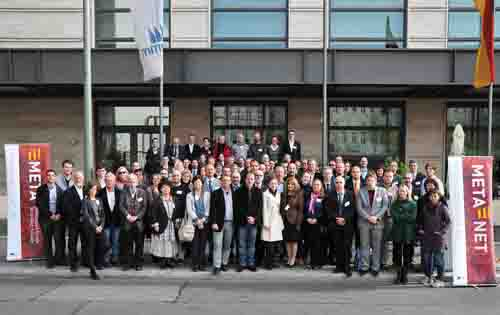
\includegraphics[width=\textwidth]{../_media/meta-net_team.jpg}
   %\fbox{Dummy -- we'll include the group photo of our META-NET meeting in Berlin here}
  \caption{Omkring 100 sprogteknologieksperter -- repr\ae sentanter for de lande og sprog, der er repr\ae senteret i META-NET -- diskuterede og afsluttede de vigtigste resultater og budskaber af hvidbogsserien \mbox{p\aa} et META-NET-m\o de i Berlin, Tyskland, oktober 21/22, 2011. --- \textcolor{grey1}{About 100 language technology experts -- representatives of the countries and languages represented in META-NET -- discussed and finalised the key results and messages of the White Paper Series at a META-NET meeting in Berlin, Germany, on October 21/22, 2011.}}
\medskip
  \colorrule{grey3}{\textwidth}{1.5pt}
\end{figure*}

\cleardoublepage

\bsection[META-NET-Hvidbogsserien -- The META-NET White Paper Series]{META-NET-Hvidbogsserien --- The META-NET\ \ \ \ \ \ White Paper Series}
\label{whitepaperseries}

\vspace*{-5mm}
\centering
  \setlength{\tabcolsep}{2.5em}
  \begin{tabularx}{\textwidth}{lllll} \toprule\addlinespace
  %\begin{tabulary}{170mm}{LLL} \toprule
  &baskisk  & Basque & euskara& \\
  &bulgarsk & Bulgarian & български& \\
  &dansk & Danish & dansk& \\
  &engelsk & English & English& \\
  &estisk & Estonian & eesti& \\
  &finsk  & Finnish & suomi& \\
  &fransk  & French & français& \\
  &galicisk & Galician & galego& \\
  &gr\ae sk & Greek & ελληνικά& \\
 &hollandsk & Dutch & Nederlands& \\
   &irsk & Irish & Gaeilge& \\
 &islandsk & Icelandic & íslenska& \\
  &italiensk & Italian & italiano& \\
  &katalansk & Catalan & català& \\
  &kroatisk & Croatian & hrvatski& \\
  &lettisk & Latvian & latviešu valoda& \\
  &litauisk & Lithuanian & lietuvių kalba& \\
  &maltesisk & Maltese & Malti& \\
  &norsk bokmål & Norwegian Bokmål & bokmål& \\
  &norsk nynorsk & Norwegian Nynorsk & nynorsk& \\
  &polsk & Polish & polski& \\
  &portugisisk & Portuguese & português& \\
  &rum\ae nsk & Romanian & română& \\
  &serbisk & Serbian & српски& \\
  &slovakisk & Slovak & slovenčina& \\
  &slovensk & Slovene & slovenščina& \\
  &spansk & Spanish & español& \\
  &svensk & Swedish & svenska& \\
  &tjekkisk & Czech & čeština& \\
&tysk & German & Deutsch& \\
  &ungarsk & Hungarian & magyar& \\ \addlinespace \bottomrule
\end{tabularx}
